%%%%%%%%%%%%%%%%%%%%%%%%%%%%%%%%%%%%%%%%%%%%%%%%%%%%%%%%%%%%%%%%%%%%%%%%%%%%%%%%%%%%%%%%%%%%%%%%%%%
% CPS 
%%%%%%%%%%%%%%%%%%%%%%%%%%%%%%%%%%%%%%%%%%%%%%%%%%%%%%%%%%%%%%%%%%%%%%%%%%%%%%%%%%%%%%%%%%%%%%%%%%%

%%%%%%%%%%%%%%%%%%%%%%%%%%%%%%%%%
% Elements  % STKLIK: comment the next two lines, because of "command already defined" error
% \newcommand{\CPSCyberPart}{\p{CyberPart}\xspace}
% \newcommand{\CPSPhysicalPart}{\p{PhysicalPart}\xspace}

%%%%%%%%%%%%%%%%%%%%%%%%%%%%%%%%%%%%%%%%%%%%%%%%%%%%%%%%%%%%%%%%%%%%%%%%%%%%%%%%%%%%%%%%%%%%%%%%%%%
% MPM 
%%%%%%%%%%%%%%%%%%%%%%%%%%%%%%%%%%%%%%%%%%%%%%%%%%%%%%%%%%%%%%%%%%%%%%%%%%%%%%%%%%%%%%%%%%%%%%%%%%%


%%%%%%%%%%%%%%%%%%%%%%%%%%%%%%%%%
% MegaModel
\newcommand{\CPSLabMM}{\p{CPSLabMM}\xspace}

% MegaModelFragments
\newcommand{\CPSLabMTMMF}{\p{CPSLabMTMMF}\xspace}
\newcommand{\CPSLabMiLMMF}{\p{CPSLabMiLMMF}\xspace}
\newcommand{\CPSLabRPaMMF}{\p{CPSLabRPaMMF}\xspace}
\newcommand{\CPSLabRPbMMF}{\p{CPSLabRPbMMF}\xspace}
\newcommand{\CPSLabSiLaMMF}{\p{CPSLabSiLaMMF}\xspace}
\newcommand{\CPSLabSiLbMMF}{\p{CPSLabSiLbMMF}\xspace}
\newcommand{\CPSLabHiLMMF}{\p{CPSLabHiLMMF}\xspace}

% Languages
\newcommand{\MATLABSimulinkLanguage}{\p{MATLAB/Simulink Language}\xspace}
\newcommand{\FESTORobotinoSimLanguage}{\p{FESTO Robotino{\copyright}Sim Language}\xspace}
\newcommand{\AUTOSARLanguage}{\p{AUTOSAR Language}\xspace}


% Models
\newcommand{\CPSLabControlModel}{\p{ControlModel}\xspace}
\newcommand{\CPSLabControlModelCode}{\p{ControlCode}\xspace}
\newcommand{\CPSLabPlantModel}{\p{PlantModel}\xspace}
\newcommand{\CPSLabRobotModel}{\p{RobotModel}\xspace}
\newcommand{\CPSLabSystemModel}{\p{SystemModel}\xspace}
\newcommand{\CPSLabSystemModelCode}{\p{SystemCode}\xspace}
\newcommand{\CPSLabSystemModels}{multiple {\CPSLabControlModel}s and one \CPSLabSystemModel\xspace}

% Tools
\newcommand{\MATLABSimulinkEditor}{\p{MATLAB/Simulink Editor}\xspace}
\newcommand{\MATLABSimulinkSimulator}{\p{MATLAB/Stateflow Simulator}\xspace}
\newcommand{\dSPACETargetLink}{\p{dSPACE TargetLink}\xspace}
\newcommand{\dSPACESystemDesk}{\p{dSPACE SystemDesk}\xspace}
\newcommand{\FESTORobotinoSim}{\p{FESTO Robotino{\copyright}Sim}\xspace}
\newcommand{\FESTORobotinoView}{\p{FESTO Robotino{\copyright}View}\xspace}
\newcommand{\DesktopExecution}{\p{Execution on a Desktop computer}\xspace}
\newcommand{\RobotExecutionLocal}{\p{Local execution on a Robotino Robot}\xspace}
\newcommand{\RobotExecutionRemote}{\p{Remote execution on a Robotino Robot}\xspace}


% =====================================================
\addtocounter{footnote}{1}
\section{HPI CPSLab$^{\thefootnote{}}$}\footnotetext[\thefootnote{}]{Acknowledgements: We thank Sebastian W{\"a}tzoldt, Stefan Neumann, Joachim H{\"a}nsel, and Falk Benke for their contributions to the lab described in this section and their contribution to the presented content and figures.}

\LEAD{Soumyadip}\ALSO{Holger, Dominique}\STATUS{%
Soumyadip has added some figures from the Pisa keynote and the BX/MX Dagstuhl seminar; 
Holger restructured the text to reflect the three stages of the ontology; 
Holger added mappings to the ontologies; 
STILL TO BE DONE: 
model the introduced ontology elements in the catalog or CPSLab ontology; 
add graphics showing the added concepts/instances of the ontologies
}

To structure the presentation of this case study according to the efforts for the MPM4CPS project, we will
%
at first in Section~\ref{subsec:cpslab-overview} provide an overview about the case study and lab,
%
then in Section~\ref{subsec:cpslab-cps} review the technical setting and derive the required needs concerning the CPS ontology,
%
thereafter in Section~\ref{subsec:cpslab-mpm} we will outline how the models, tools, and tool chain employed in the case study can be captured as multi-paradigm modeling and derive the required needs concerning the MPM ontology, and
%
finally in Section~\ref{subsec:cpslab-mpm4cps} we discuss how the CPS character of the case study is reflected in its multi-paradigm modeling and the use of the MPM4CPS ontology.

% ========================================================================================
\subsection{Overview}\label{subsec:cpslab-overview}


As outlined in more details from a conceptual point of view\uidx{ViewPoint} in \cite{Waetzoldt:2012pa}, the presented \emph{CPSLab}\footnote{http://www.cpslab.de} at the Hasso Plattner Institute (HPI)\footnote{http://www.hpi.de} at the University of Potsdam applied, adapted, and evaluated an existing industrial-strength development methodology from the automotive domain \cite{Broekman&Notenboom2003} (see also Figure~\ref{fig:methodology}) for the robotic system application domain\uidx{ApplicationDomain}. We therefore evaluated and adapted a component-based\uidx{Component} approach using an MDE approach supporting the combination of soft and hard real-time behavior\uidx{BehaviouralCharacteristic}.

\begin{figure}[!htb]
\centering
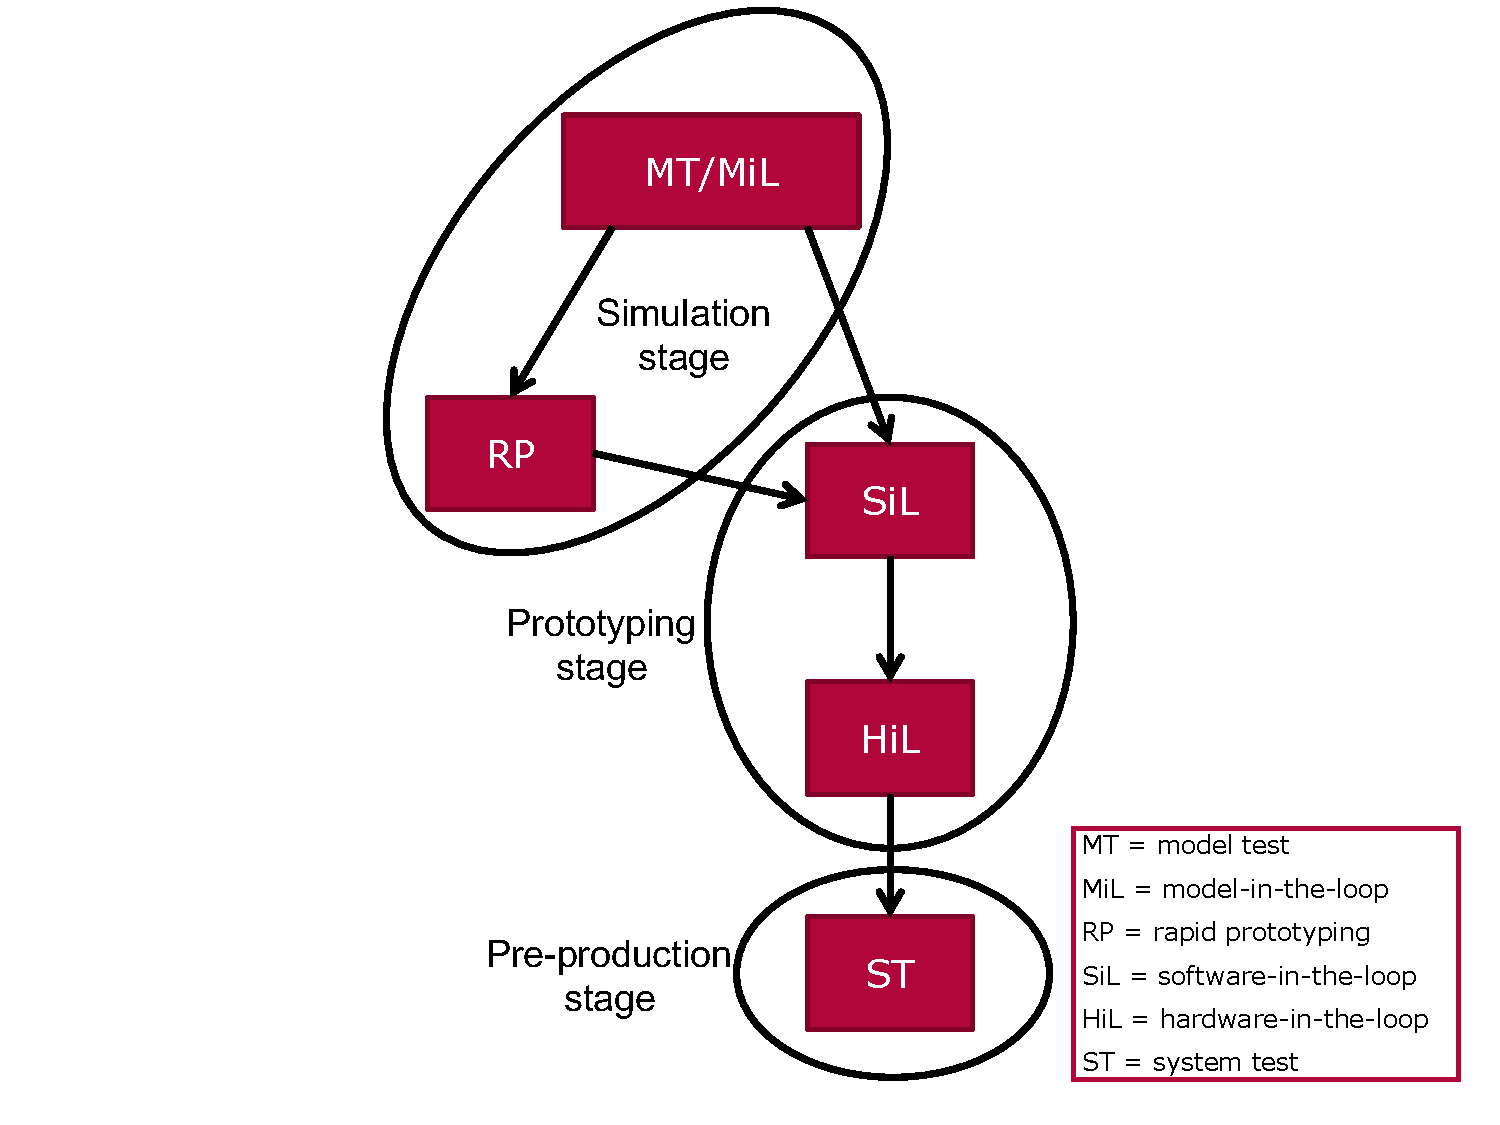
\includegraphics[width=0.66\textwidth]{figures/methodology.pdf}
\caption{Overview of the methodology for modeling, verification, and validation employing simulation and testing (see \cite{Broekman&Notenboom2003})}
\label{fig:methodology}
\end{figure}

The resulting methodology for robotic systems supports several development activities such as modeling, simulation, verification/testing at different stages, prototyping and pre-production. The lab supports tools and related libraries in an integrated tool-chain that reflects physical and cyber aspects of distributed\uidx{Distributed} robotics systems.

\begin{figure}[!htb]
\centering
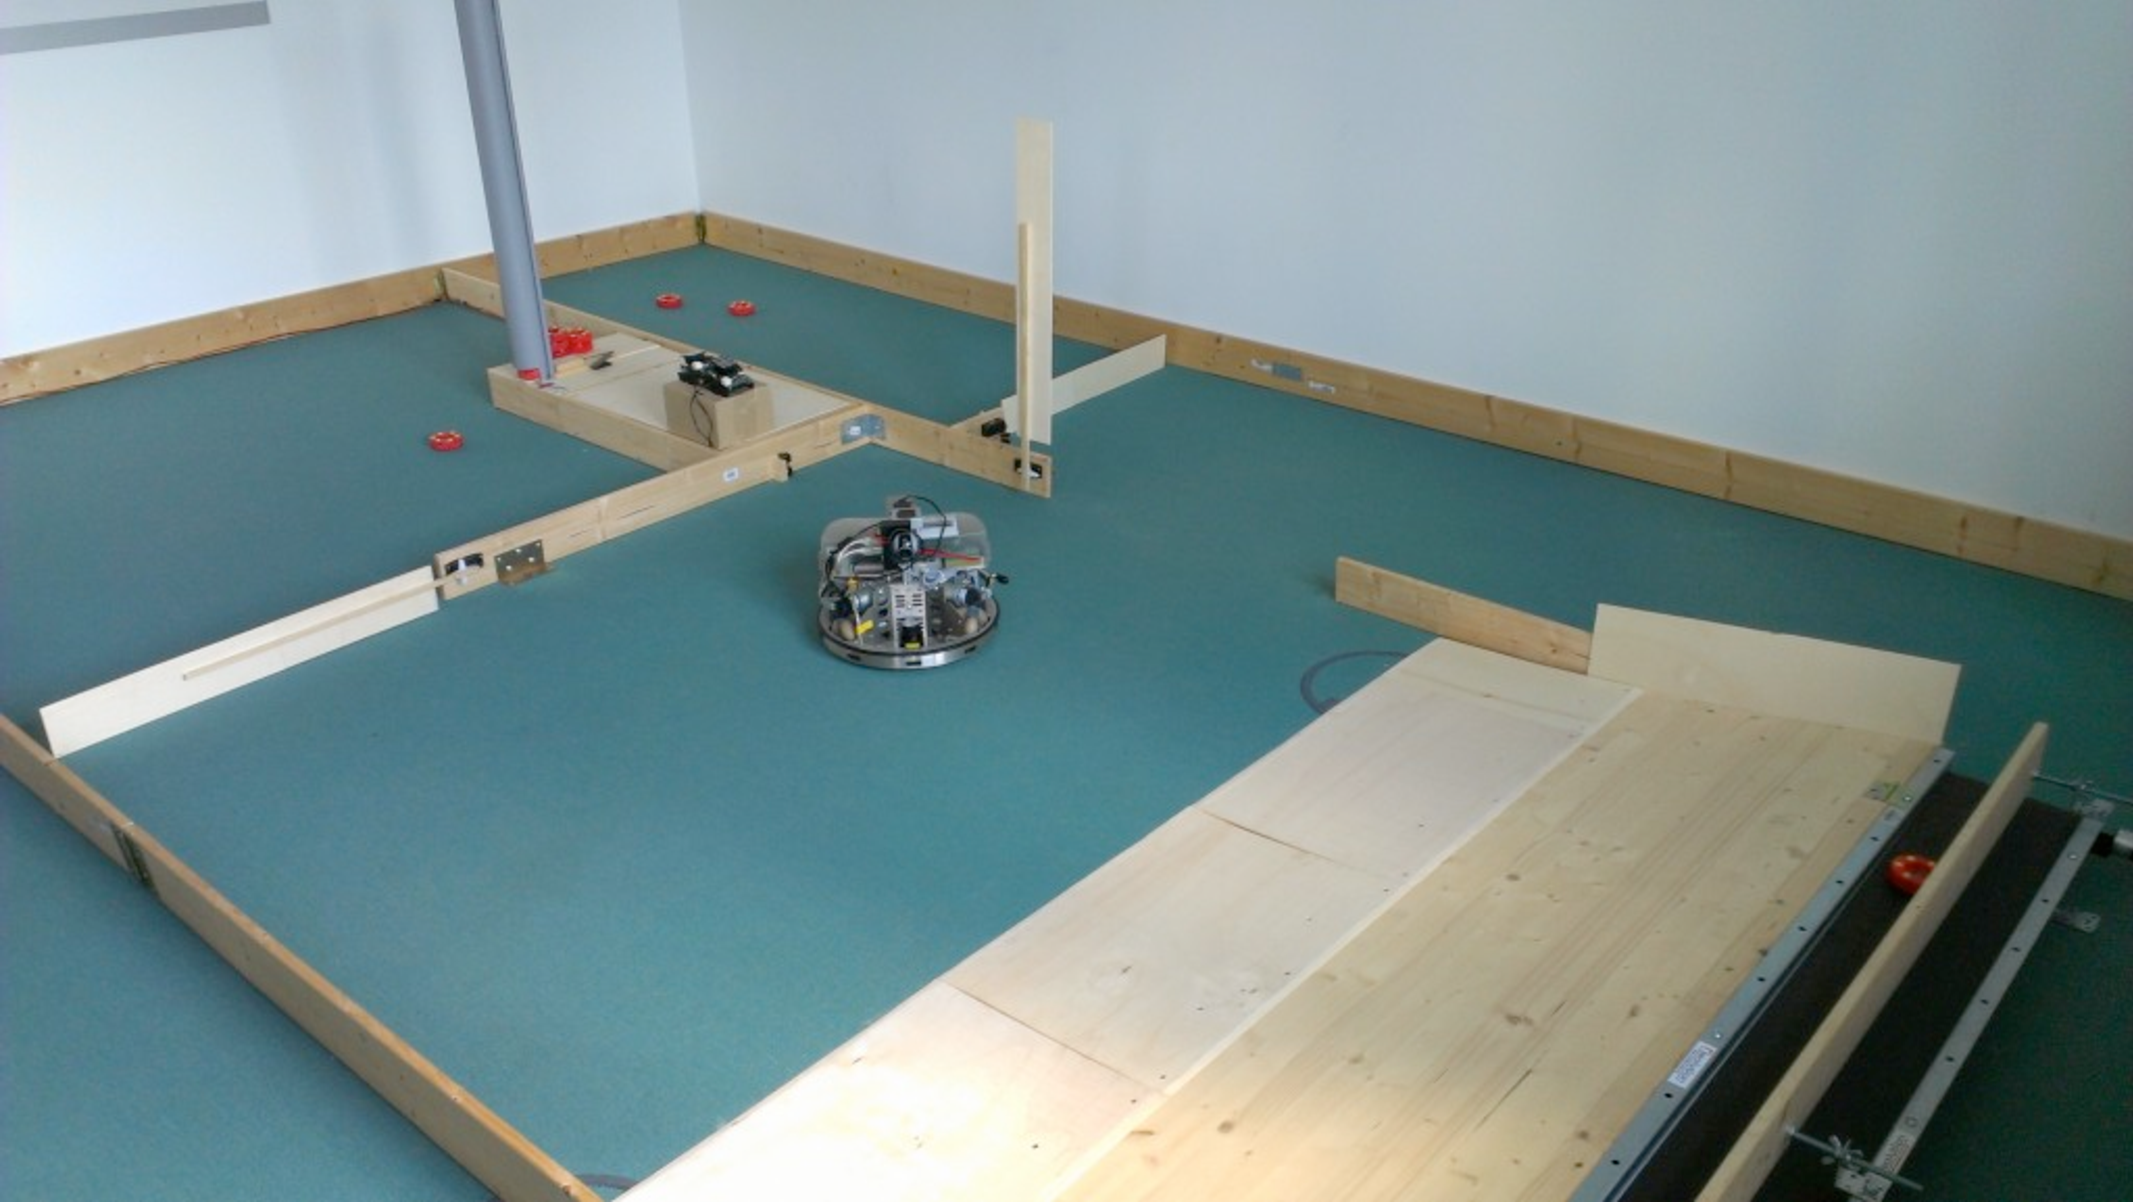
\includegraphics[width=0.8\textwidth]{figures/evaluation_scenario_2.pdf}
\caption{Photo of the lab (see \cite{Waetzoldt:2012pa})}
\label{fig:evaluation_scenario_2}
\end{figure}


We consider a robot system as depicted in Figure~\ref{fig:evaluation_scenario_2}, where a single robot has the duty to transport pucks as advised by the overall factory automation. The regular behavior of the robot is to move around, transport pucks, or charge its batteries. The behavior must meet strict constraints, such as preventing complete discharge of the batteries and with a lower priority, ensure to transport pucks as requested. It must also perform reasonably well with respect to some soft goals to minimize energy consumption and maximize throughput.

\begin{figure}[!htb]
\centering
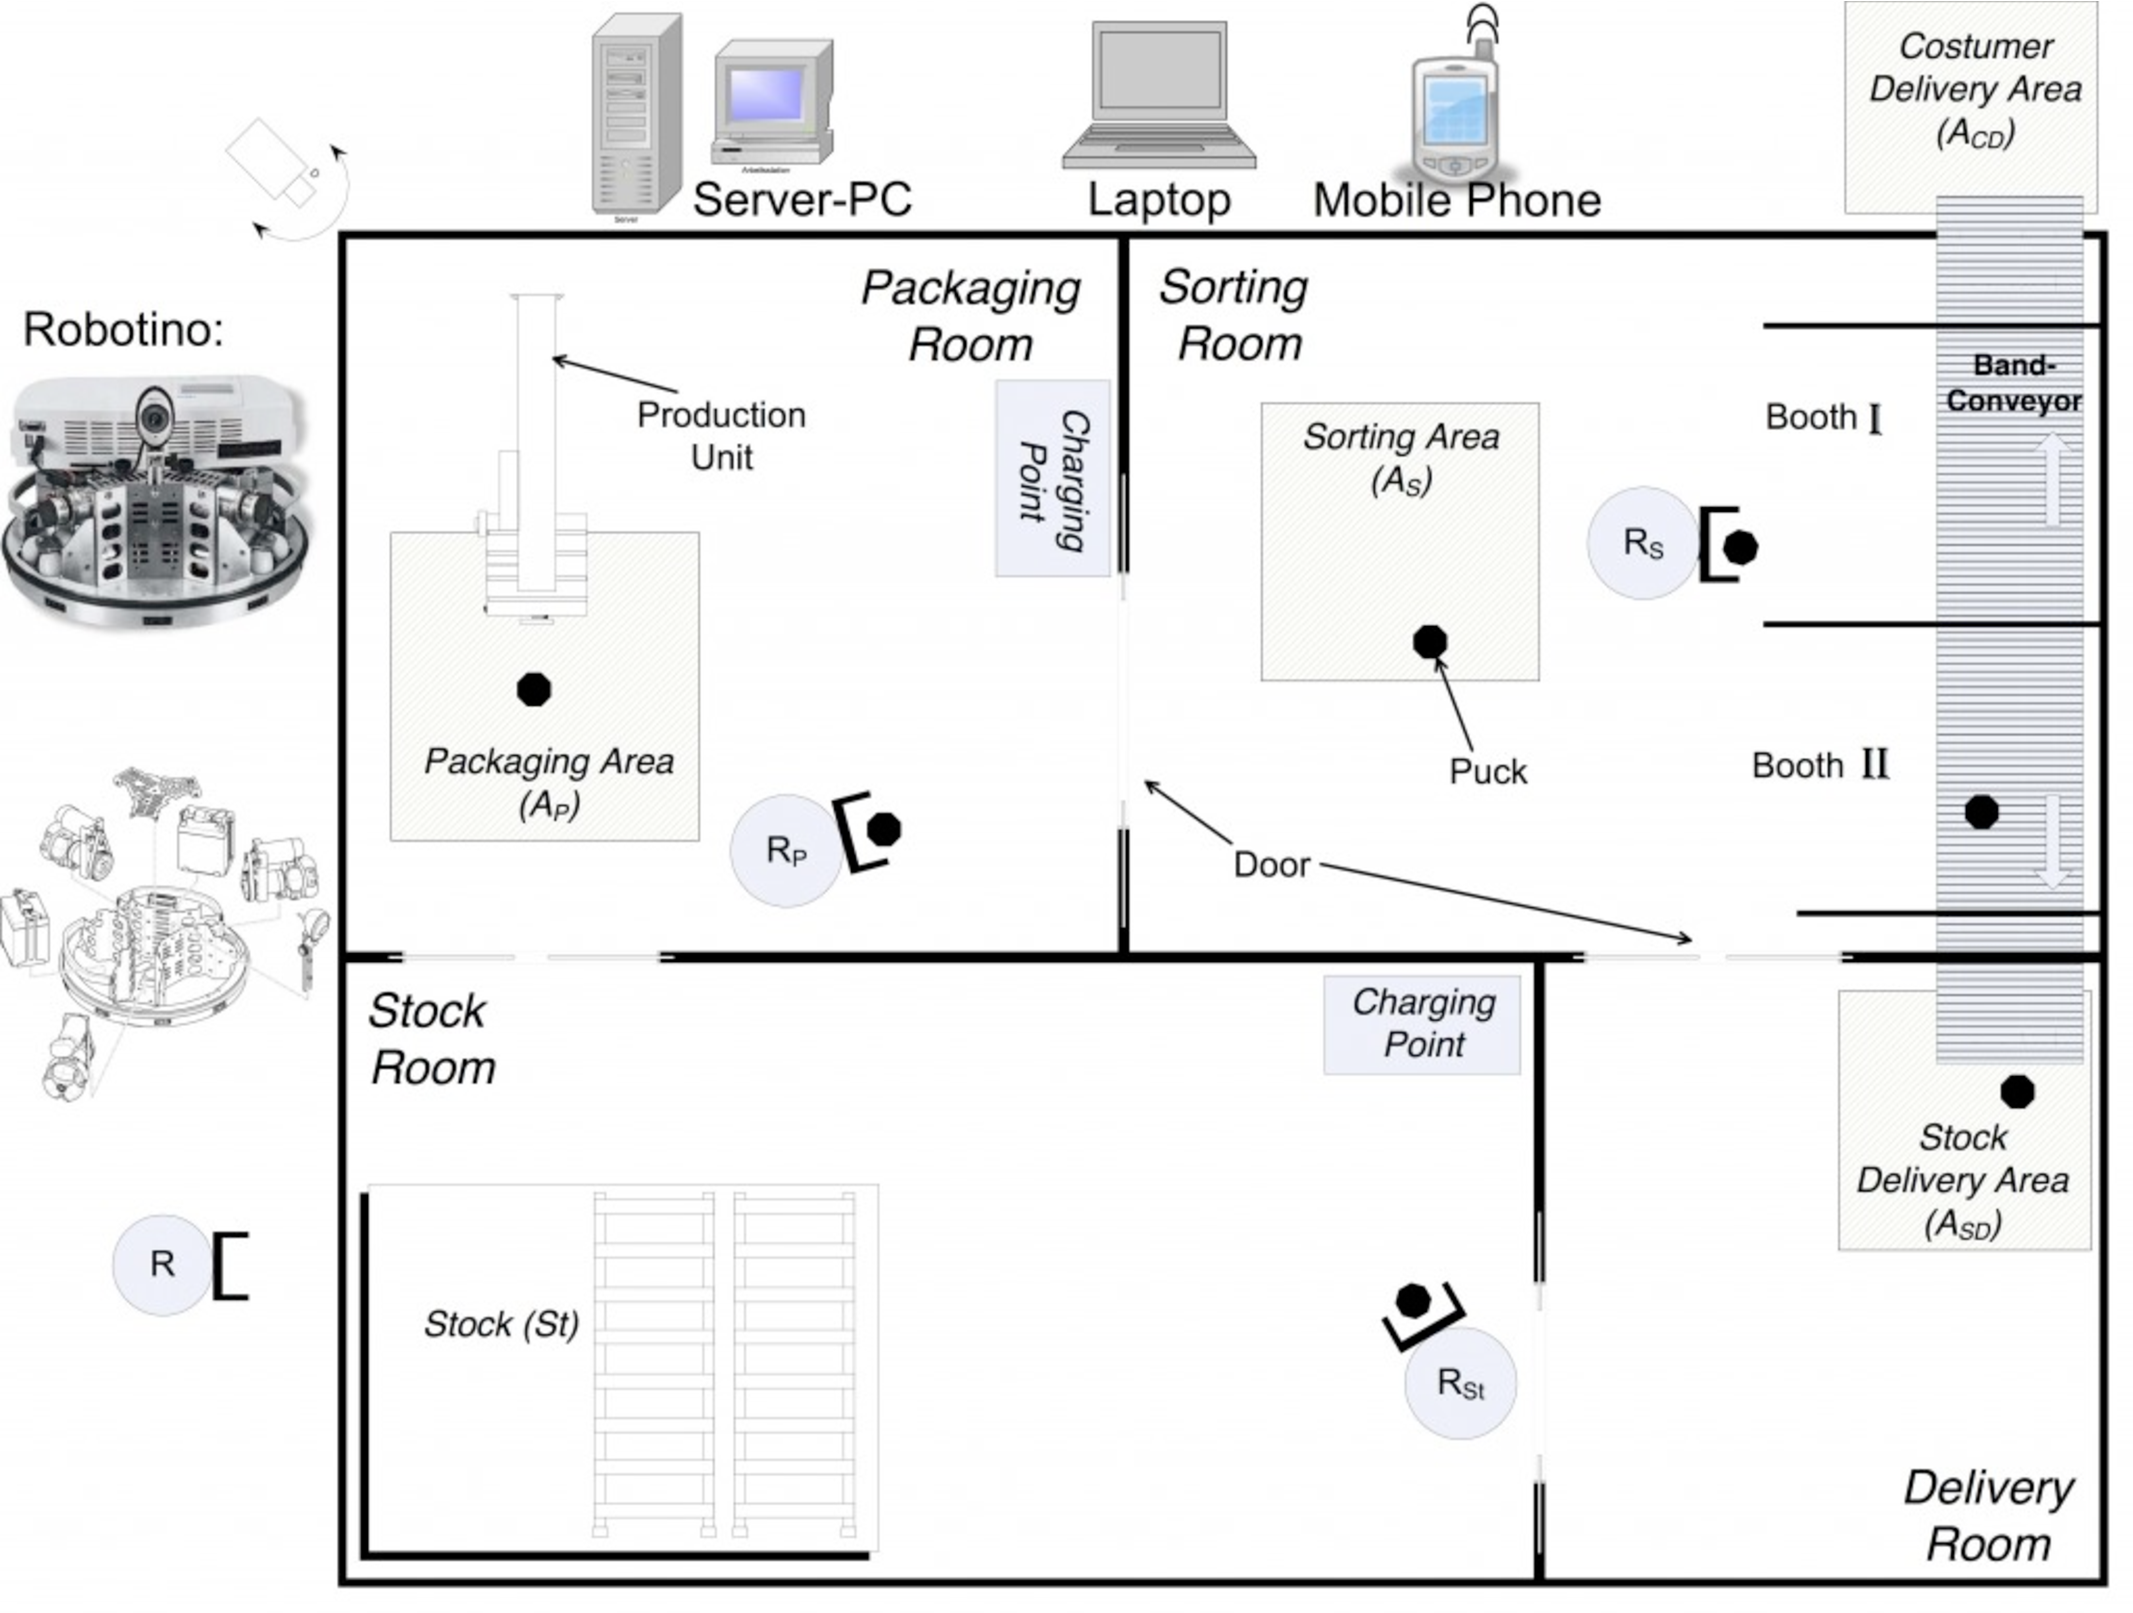
\includegraphics[width=0.8\textwidth]{figures/evaluation_scenario_1.pdf}
\caption{Structural\uidx{StructureCharacteristic} overview of the employed evaluation scenario (see \cite{Waetzoldt:2012pa})}
\label{fig:evaluation_scenario_1}
\end{figure}

Figure~\ref{fig:evaluation_scenario_1} depicts a structural\uidx{StructureCharacteristic} overview of the robot system. The whole cyber-physical evaluation scenario consists of four different rooms. In the first room, the pucks are packed and dropped for transportation in area $A_P$. A robot $R_P$ transports the puck to a second room and drops it within the sorting area $A_S$. Based on the current delivery status, the robot $R_S$ chooses one of the two booths and a band-conveyor transports the puck to the customer or stock delivery area ($A_{CD}$, $A_{SD}$) afterwards. In a third step, the robot $R_{St}$ transfers the puck to stock in $St$. The doors can be opened or closed dynamically to vary the scenario. A robot can charge its battery at one of the two charging points. Each robot acts as an autonomous unit. Therefore, the tasks transportation, sorting and stocking are independent from each other.

\begin{figure}[!htb]
\centering
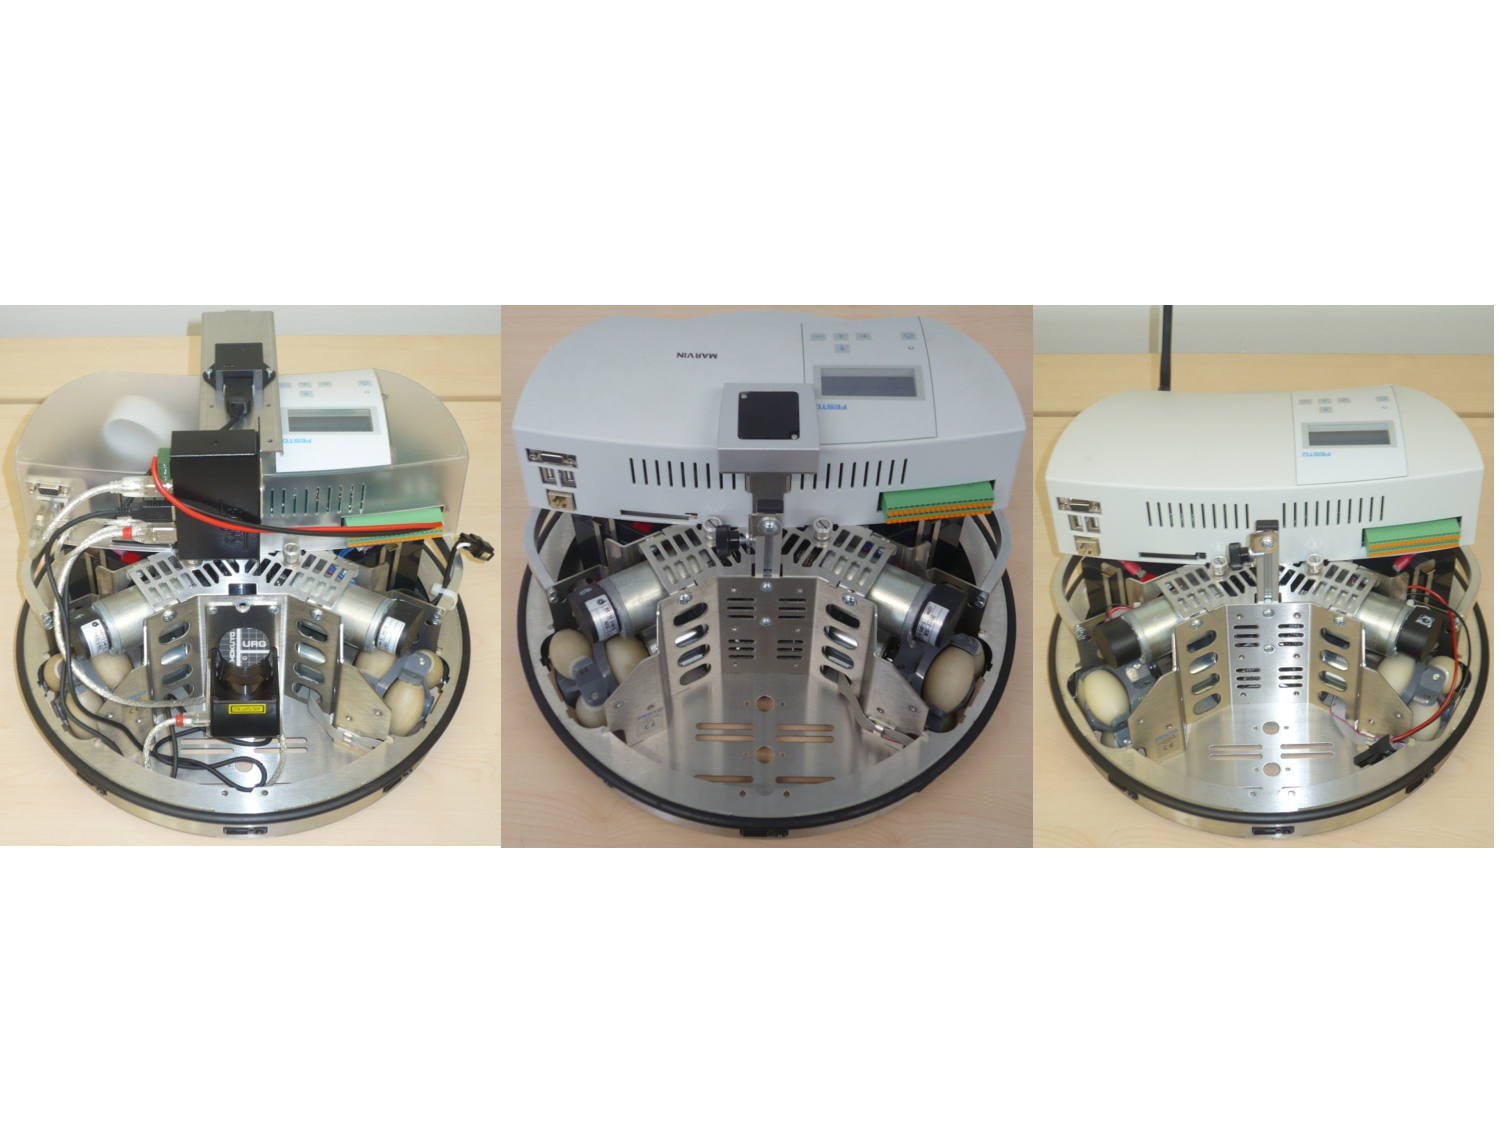
\includegraphics[width=0.8\textwidth]{figures/evaluation_scenario_3.pdf}
\caption{Photo of the employed robots (see \cite{Waetzoldt:2012pa})}
\label{fig:evaluation_scenario_3}
\end{figure}


For the evaluation of our research activities, we use our CPSLab robot laboratory consisting of three Robotino robots (see Figure~\ref{fig:evaluation_scenario_3}). The robots can be equipped with several sensors (e.g., laser scanner, infrared (IR) distance sensors, GPS-like indoor navigation systems) as well as different actuators (e.g., servo motors, omnidirectional drive, gripper). 

The general idea of our evaluation scenario is the realization of a variable production setting, where robots can transport small pucks (representing goods in a production system) to different locations. The robots must fulfill different requirements, e.g., they must provide basic functionality like moving and avoiding obstacles in hard real-time (reacting on obstacles within a few milliseconds). Further, the robots must achieve high level goals, e.g., energy saving of the battery, short routing to the destination points and optimizing the throughput while transporting the pucks. While basic functionalities, such as obstacle avoidance, must be realized in hard real-time, we use existing libraries to realize higher functionalities such as path planning or creating a map by evaluating measured distance values. The latter can rarely be realized under hard real-time constraints\uidx{Constraint} because of insufficient libraries. Furthermore, we run a RTAI Linux operating system on the robot to enable hard real-time execution.

% ========================================================================================
\subsection{CPS}\label{subsec:cpslab-cps}

In the following, we will use the details of the different development steps to outline how the development is linked to CPS and the concepts of the CPS ontology introduced in Chapter~\ref{ch:cps}.

% ============================================
\subsubsection{Simulation Stage}
%
The first step of the development process\uidx{Process} of Figure~\ref{fig:methodology} is a simulation stage that focus on the model development resp.~functional development for the employed control laws.
%
At this stage, many details resulting from the physical and cyber parts of the system are ignored resp.~simplified such as real sensor values with noise, specific effects of scheduling, the impact of communication interaction and messages, and timing/memory/computation constraints.

\begin{figure}[!htb]
\centering
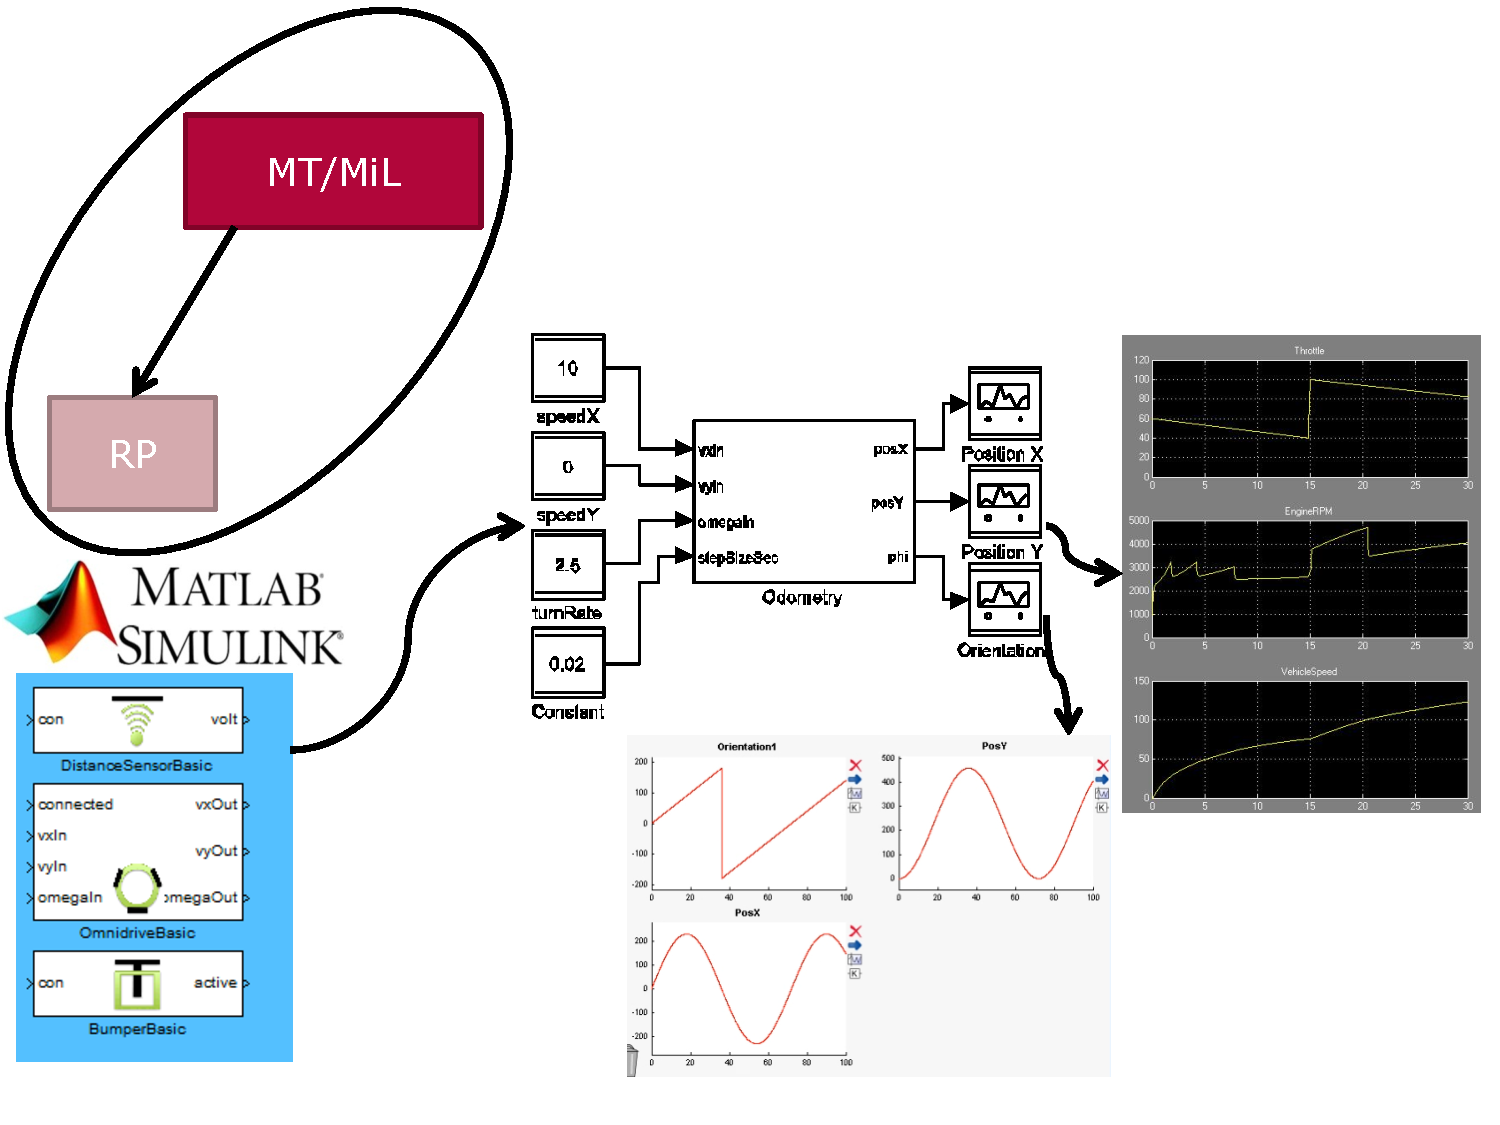
\includegraphics[scale=0.33]{figures/mt.pdf}
\caption{Overview of the model test in the simulation stage of \cite{Broekman&Notenboom2003}}
\label{fig:mt}
\end{figure}

% =========================================
\subsubsubsection{Model Test}
%
In a first activity\uidx{Activity} named \emph{model test} (MT)\uidx{ModelingActivity} (see Figure~\ref{fig:mt}), a so-called one-way/one-shot simulation with MATLAB/Simulink is supported where the model of the control behavior can be stimulated by inputs to see that they react properly. This provides some confidence that the setup control behavior works as intended.

% =========================================
\subsubsubsection{Model Test - CPS Ontology}
%
In the model test as outlined in Figure~\ref{fig:mt}, the abstract control algorithm from the cyber domain for a specific function is confronted with the physics as present in the input data plus expected outcomes relevant for the function and thus we have a very simple cyber-physical setting. 
%
Thus we cover the elements \CPSCyberPart from the CPS ontology for a particular function.


\begin{figure}[!htb]
\centering
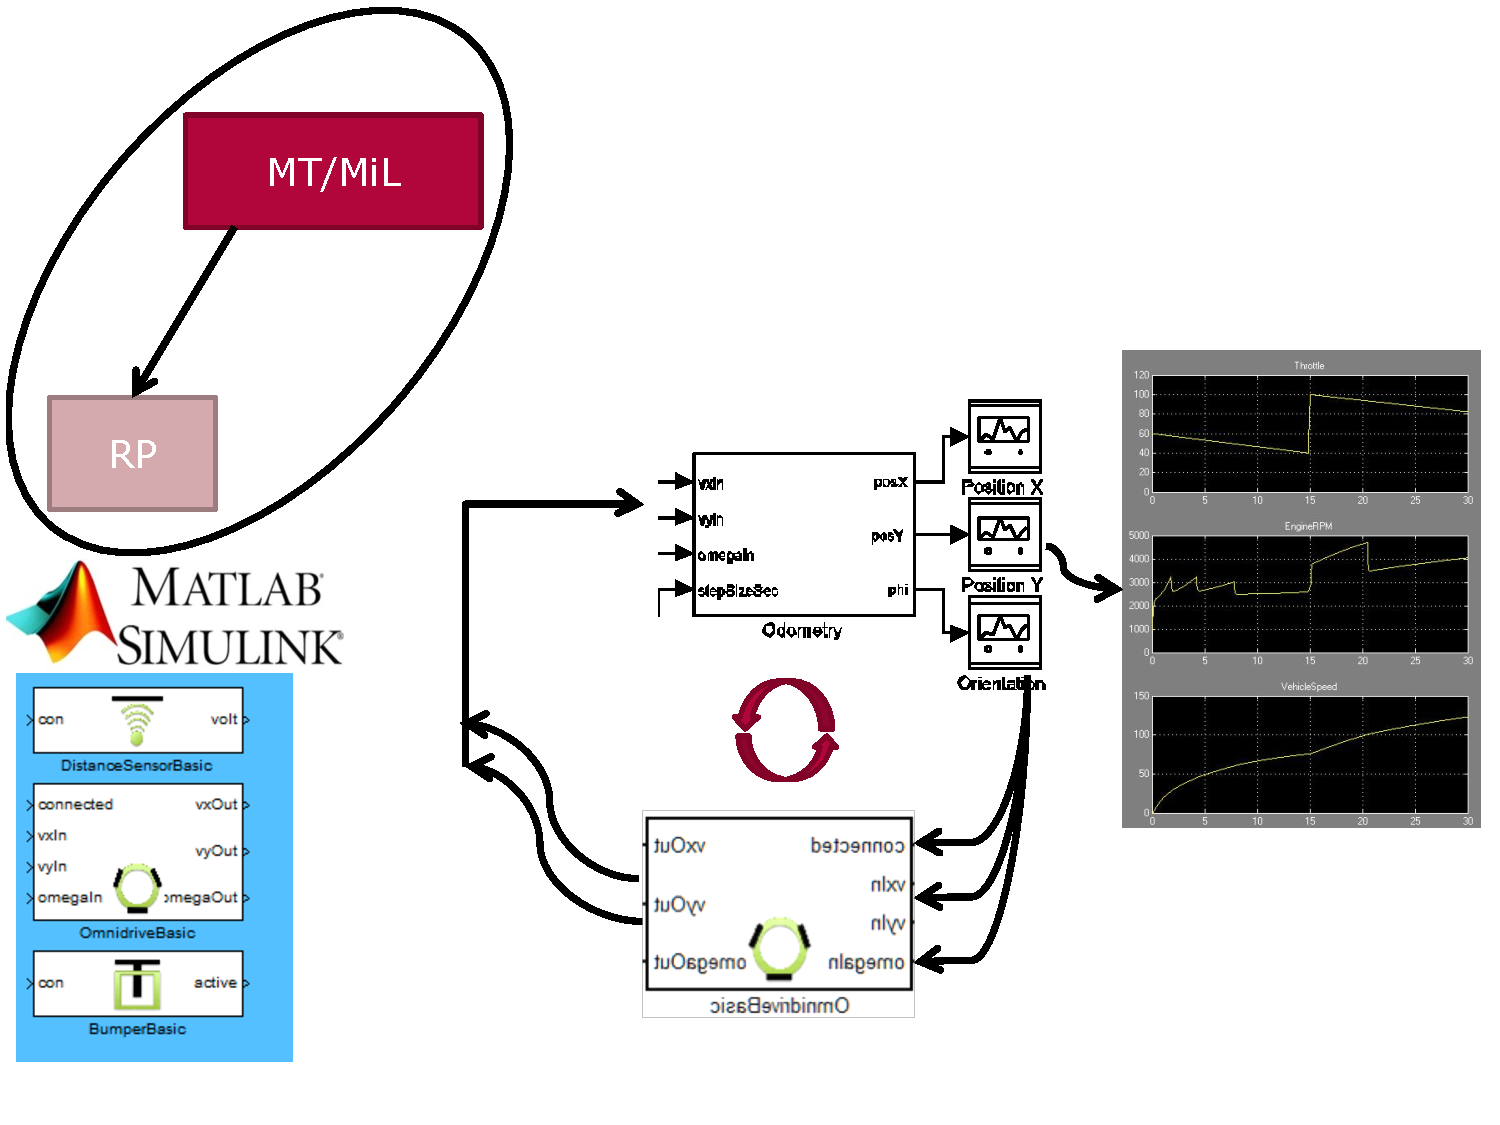
\includegraphics[scale=0.33]{figures/mil.pdf}
\caption{Overview of the model in loop simulation in the simulation stage of \cite{Broekman&Notenboom2003}}
\label{fig:mil}
\end{figure}


% =========================================
\subsubsubsection{Model-in-the-Loop}
%
In a second step, the model of the control behavior is combined with a MATLAB/Simulink model of the plant by means of a \emph{model-in-the-loop} (MiL) simulation as shown in Figure~\ref{fig:mil}, which uses the feedback provided by the plant model to evaluate that the control behavior is as expected. 

% =========================================
\subsubsubsection{Model-in-the-Loop - CPS Ontology}
%
The model in the loop depicted in Figure~\ref{fig:mil} in contrast, the abstract control algorithm from the cyber domain is combined with the idealized physics as present in the plant model and thus we have a simple cyber-physical setting. 
%
Here we cover thus the elements \CPSCyberPart and \CPSPhysicalPart from the CPS ontology for a particular function.



\begin{figure}[!htb]
\centering
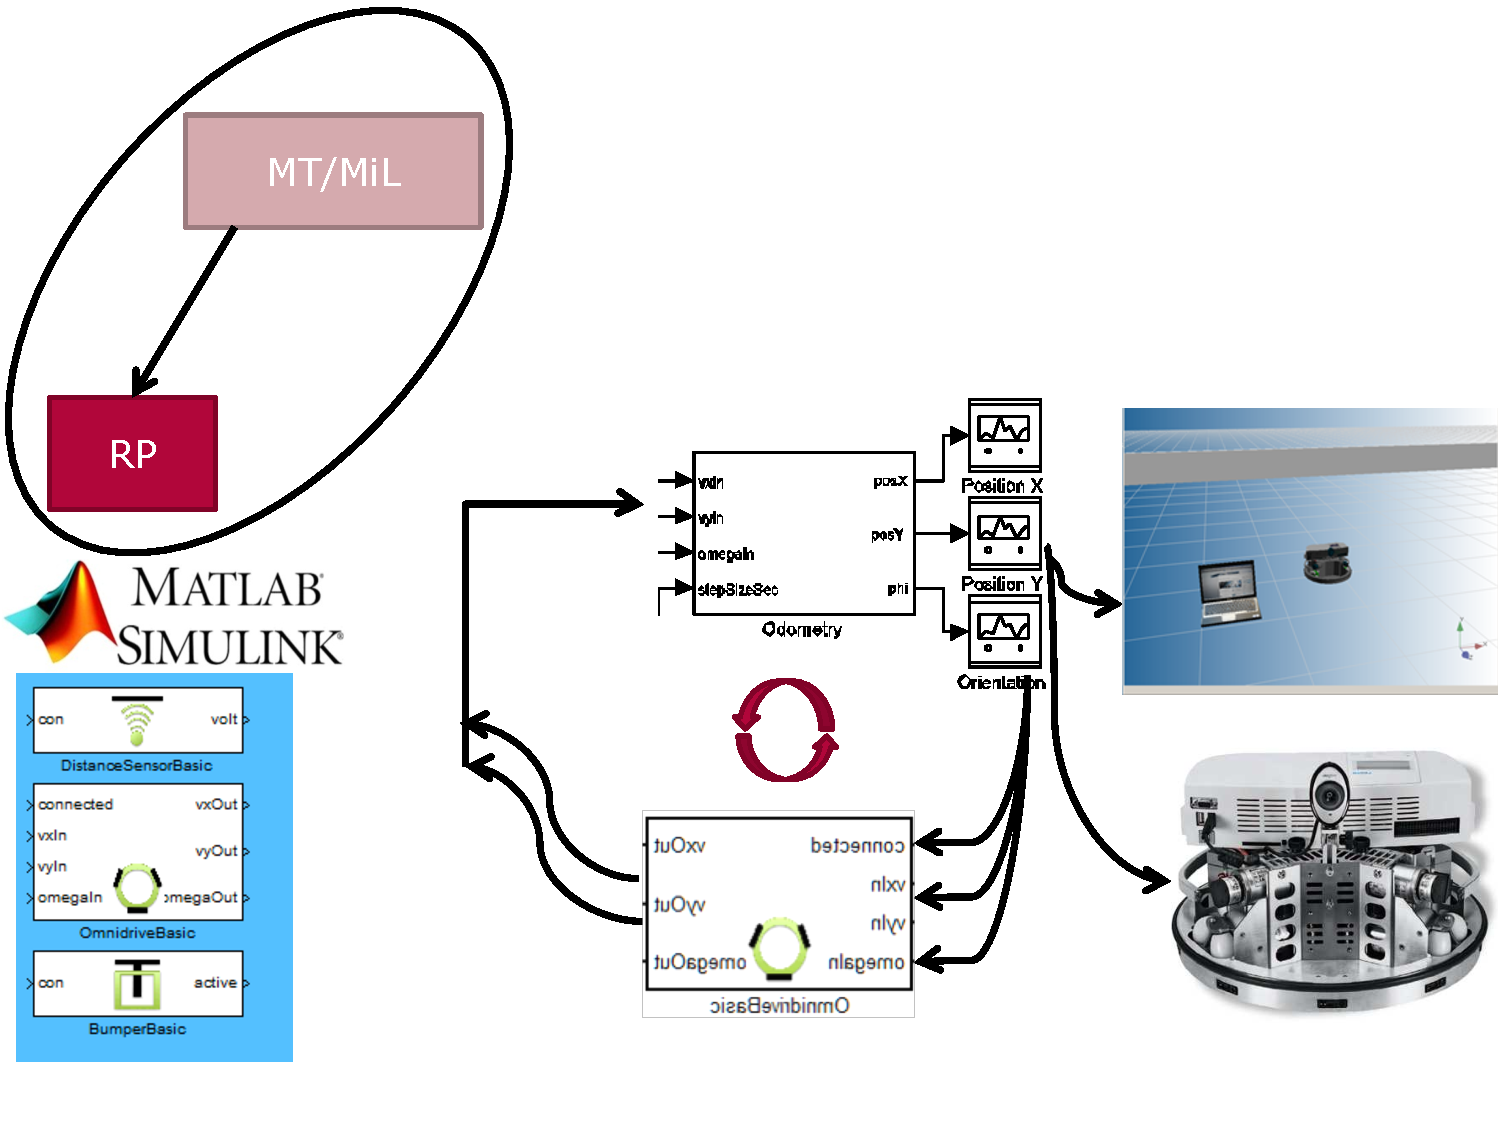
\includegraphics[scale=0.33]{figures/rp.pdf}
\caption{Overview of the rapid prototyping in the simulation stage of \cite{Broekman&Notenboom2003}}
\label{fig:rp}
\end{figure}



% =========================================
\subsubsubsection{Rapid Prototyping}
%
As the validity of plant models is often only rather limited when it comes to sophisticated aspects of the physical behavior\uidx{BehaviouralCharacteristic}, as an additional step \emph{rapid prototyping} as depicted in  Figure~\ref{fig:rp} is supported. 
%
For smaller control behavior, the model of the control behavior is linked to the real robot such that real sensor values with noise and timing constraints\uidx{Constraint} of the environment and platform can be covered. However, specific effects of scheduling, the impact of communication interaction and messages, and memory/computation constraints remain uncovered.
%
For larger scenarios and for the multi robot scenarios a link to a real hardware setup is not feasible here. Instead we employ a model-in-the-loop (MiL) simulation where a complex environment and the communication\uidx{Communication} between the robots can be explored. While this covers the impact of communication interaction and messages, other aspects like real sensor values with noise, specific effects of scheduling and timing/memory/computation constraints are, however, not covered.

% =========================================
\subsubsubsection{Rapid Prototyping - CPS Ontology}
%
The rapid prototyping against the robot as depicted in Figure~\ref{fig:rp}, the abstract control algorithm from the cyber domain is brought together with the real physics of the robot  and thus we have clearly a cyber-physical setting. 

Our rapid prototyping being based on a sophisticated robot simulator, again the abstract control algorithm from the cyber domain is brought together with the physics as present in the sophisticated robot model of the simulator and thus we have clearly a cyber-physical setting. 

In both cases we thus cover the elements \CPSCyberPart from the CPS ontology for a particular function and the elements \CPSPhysicalPart from the CPS ontology for the part of the robot relevant for a particular function that is either simulated or considered directly.






% ============================================
\subsubsection{Prototyping Stage}
%
The second supported stage is the prototyping stage where the focus changes from models to their implementation in software or hardware and where besides the individual functions also the system architecture is covered. Due to this refined view, in particular discretization effects of the cyber part\uidx{SystemPart} that are absent in the abstract mathematical models employed in the former stage now become visible.
%
At this stage, less details are ignore resp.~simplified as step by step specific effects of scheduling, the impact of communication\uidx{Communication} interaction and messages, and timing/memory/computation constraints\uidx{Constraint} are taken into account.


\subsubsubsection{More Detailed Modeling}
%
To consider the more detailed view\uidx{View} outlined, at the prototyping stage the models must be refined such that besides the individual functions also the system architecture is defined.

\begin{figure}[!htb]
\centering
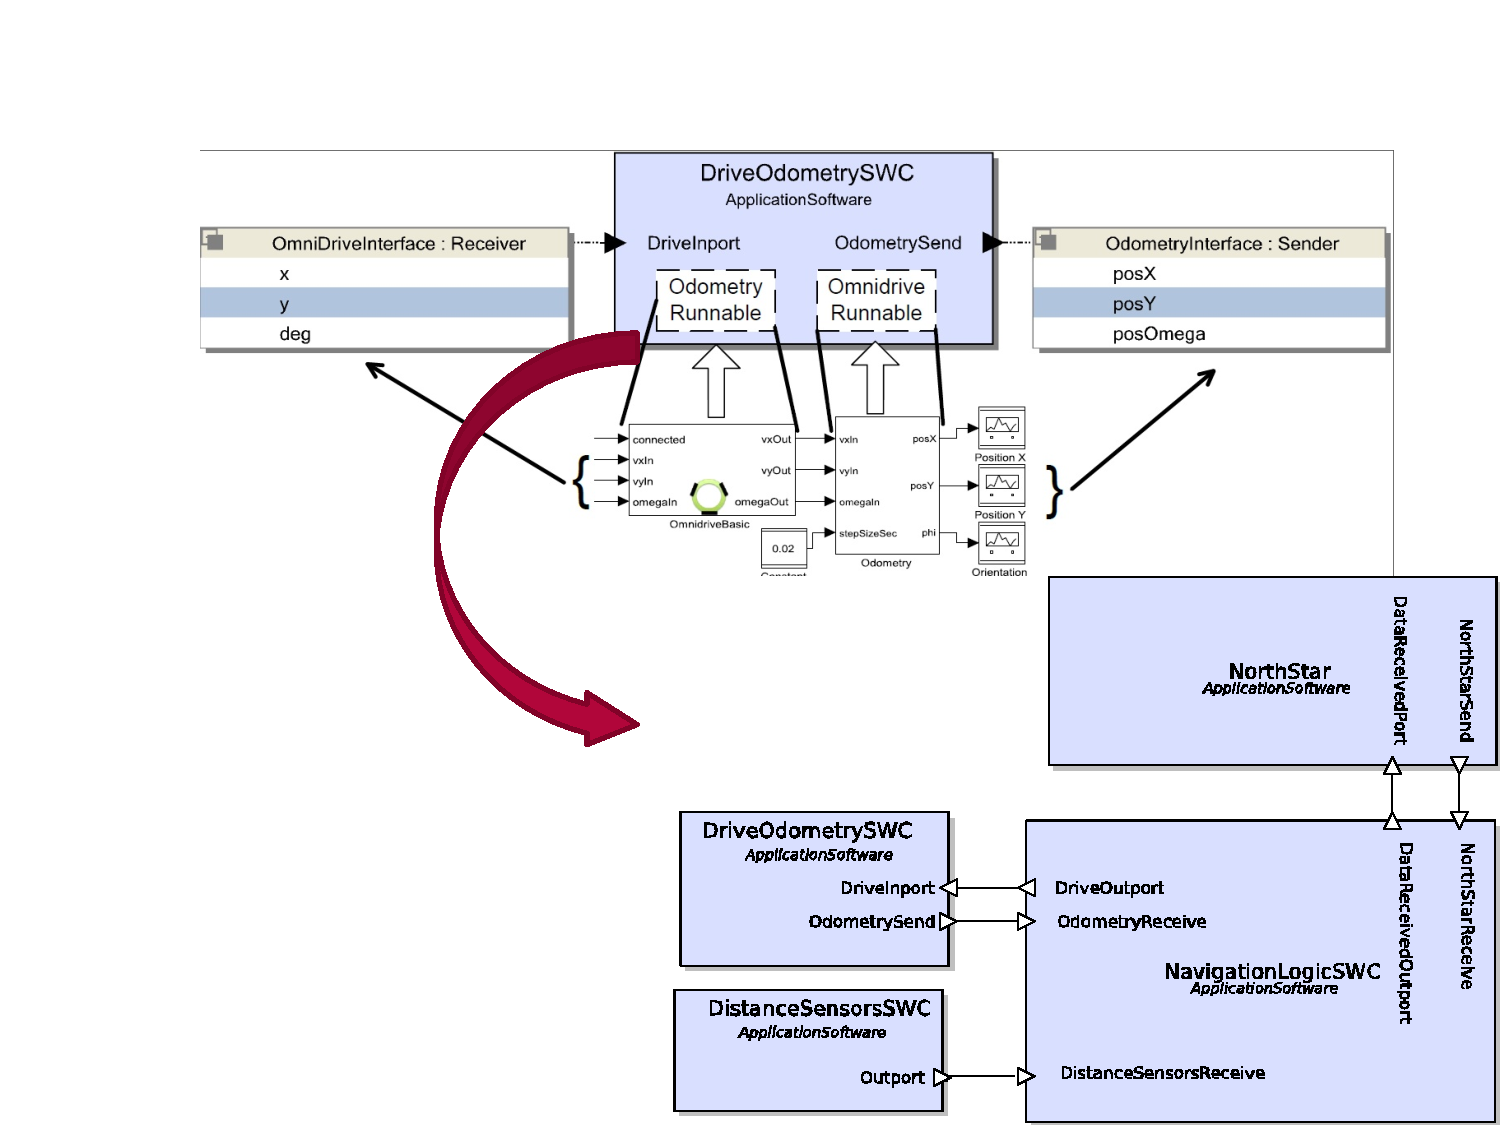
\includegraphics[scale=0.33]{figures/arch.pdf}
\caption{Overview of the definition of the software architecture in the prototyping stage of \cite{Broekman&Notenboom2003}}
\label{fig:arch}
\end{figure}

As depicted in Figure~\ref{fig:arch}, this is done by first defining components\uidx{Component} and their communication\uidx{Communication} via port types, messages, interfaces, and data types with AUTOSAR and map the beforehand considered functional parts on them. In this step, we also have to map the functionality extending the existing models and where necessary add custom implementation files.
%
In a second step, we then define the overall architecture using AUTOSAR including besides the components and their communication also task specification and the hardware configuration.


\begin{figure}[!htb]
\centering
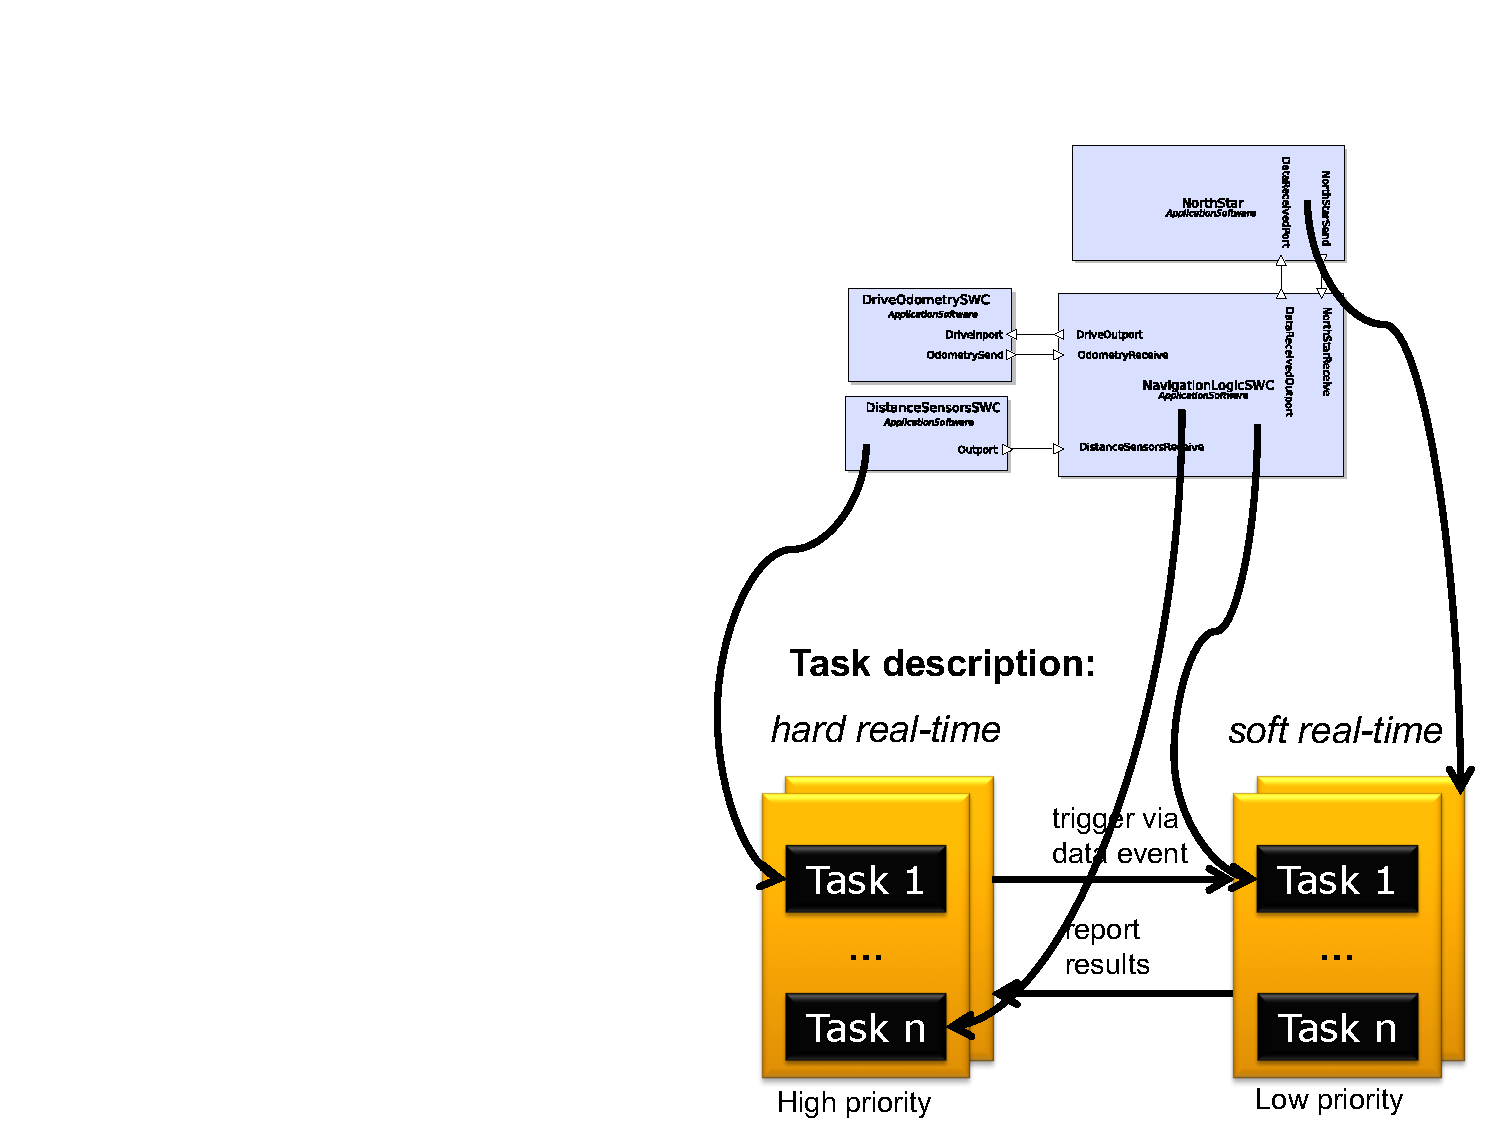
\includegraphics[scale=0.33]{figures/map.pdf}
\caption{Overview of the mapping of the architecture to tasks and communication\uidx{Communication} in the prototyping stage of \cite{Broekman&Notenboom2003}}
\label{fig:map}
\end{figure}

As depicted in Figure~\ref{fig:map}, an important element of this refinement is also real-time constraints, e.g. to guarantee safety\uidx{Safety} constraints\uidx{Constraint}. A combination of hard and soft real-time aspects at functional as well as architectural levels must be defined including a mapping to hard and soft real-time task with proper levels for the priorities.
%Where necessary such a refinement has to preserves hard real-time constraints for basic functions and the communication has to be designed such that it also is not in conflict with any hard real-time constraints and that the interaction between hard and soft real-time behavior ensures consistent and timely data exchange.


%\subsubsubsection{Verification}
%\subsubsubsection{SiL}
%
Concerning the verification, we employ code generation at the prototyping stage and try to step by step add more and more details of the software and hardware to the picture in the following steps.

\begin{figure}[!htb]
\centering
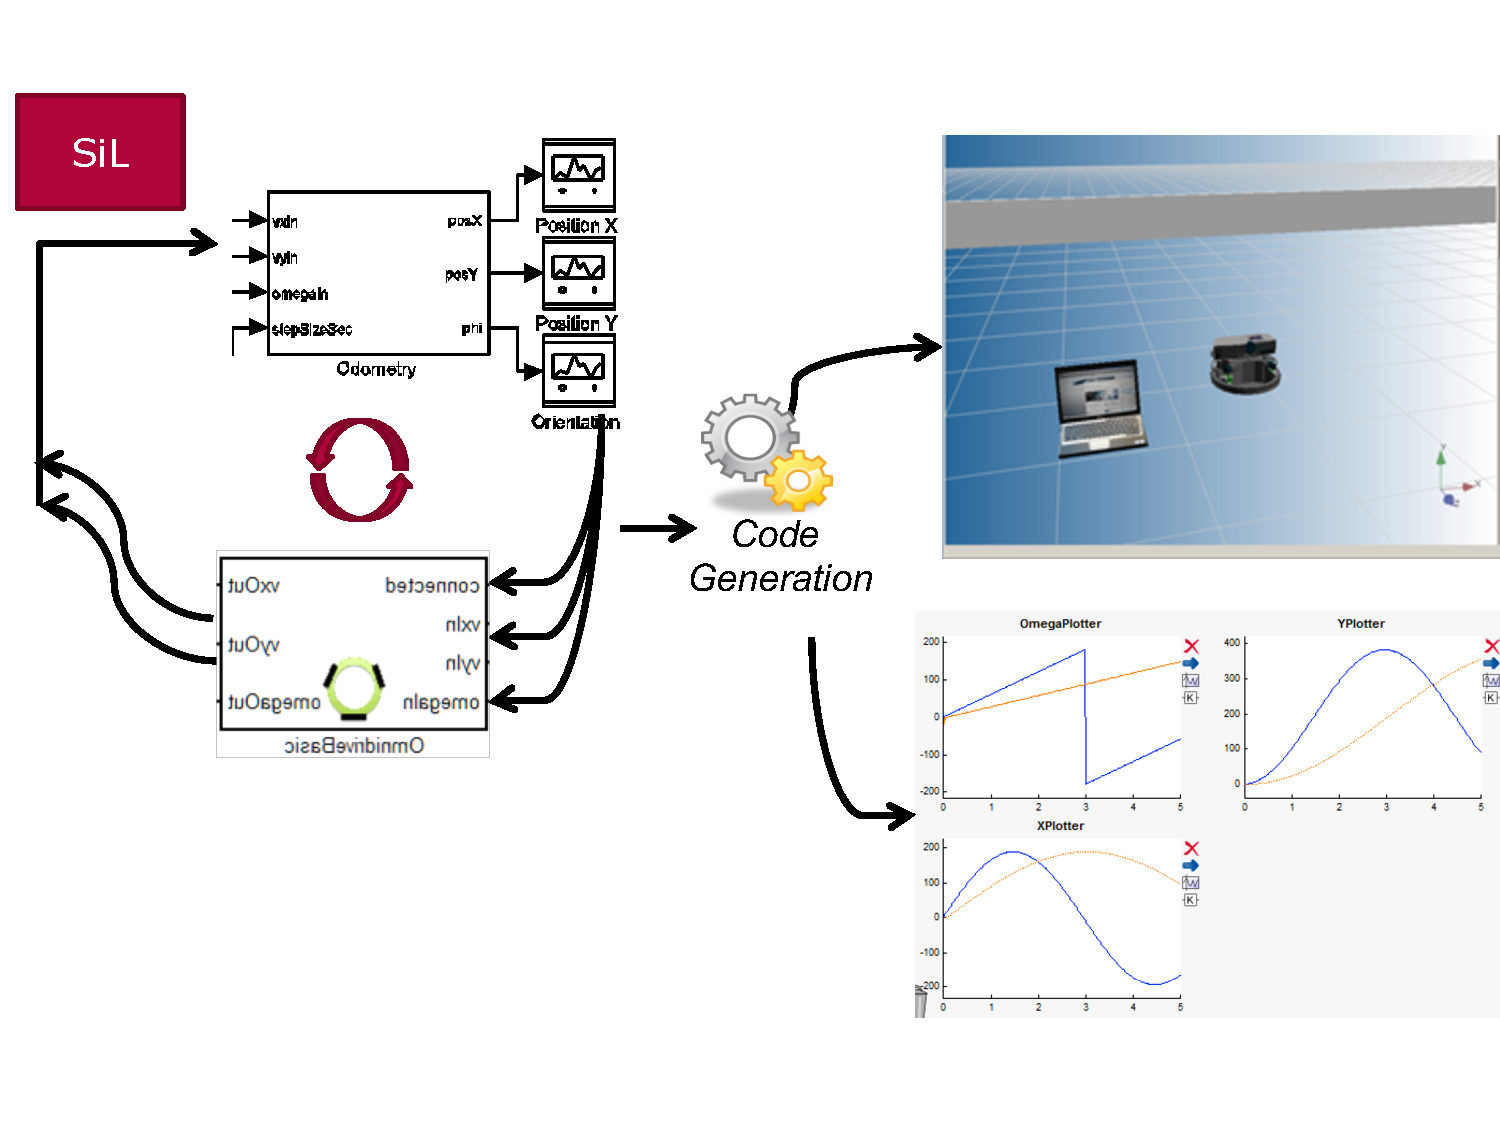
\includegraphics[scale=0.33]{figures/sil.pdf}
\caption{Overview of software-in-the-loop (sil) simulation in the prototyping stage of \cite{Broekman&Notenboom2003}}
\label{fig:sil}
\end{figure}



% ============================================
\subsubsubsection{Software in the Loop (SiL)}
%
The \emph{software-in-the-loop} (SiL) simulation at the prototyping stage as depicted in Figure~\ref{fig:sil} requires that code generation is employed to derive code for the functional models and architectural models. In special cases, also additional manually developed code has to be integrated. Then, the code is executed and run against the available simulation of the robot and its environment.

As we still do not always use the real hardware, we still ignore resp.~simplify elements such as real sensor values with noise and not by the simulator covered timing constraints\uidx{Constraint} of the environment or platform, while specific effects of scheduling, the impact of communication\uidx{Communication} interaction and messages, and by the simulator covered timing constraints of the environment or platform, and timing/memory/computation constraints of the software.
\todo{DB: This sentence is not clear}

% ============================================
\subsubsubsection{Software in the Loop (SiL) - CPS Ontology}
%
The first form of software in the loop (SiL) for which the software is executed on a desktop computer against a robot simulator features that the detailed control algorithm from the cyber domain is brought together with the physics as present in the sophisticated robot model of the simulator. Therefore, we clearly have a cyber-physical setting. 

The second form of SiL for which the software is also executed on a desktop computer but against a remotely controlled robot makes that the detailed control algorithm from the cyber domain is brought together with the physics as present in the remotely controlled robot. Therefore, we clearly have a cyber-physical setting. 

In both cases we cover the elements \CPSCyberPart from the CPS ontology for the combination of all function and the elements \CPSPhysicalPart from the CPS ontology for the whole robot.

%\subsubsubsection{HiL}

\begin{figure}[!htb]
\centering
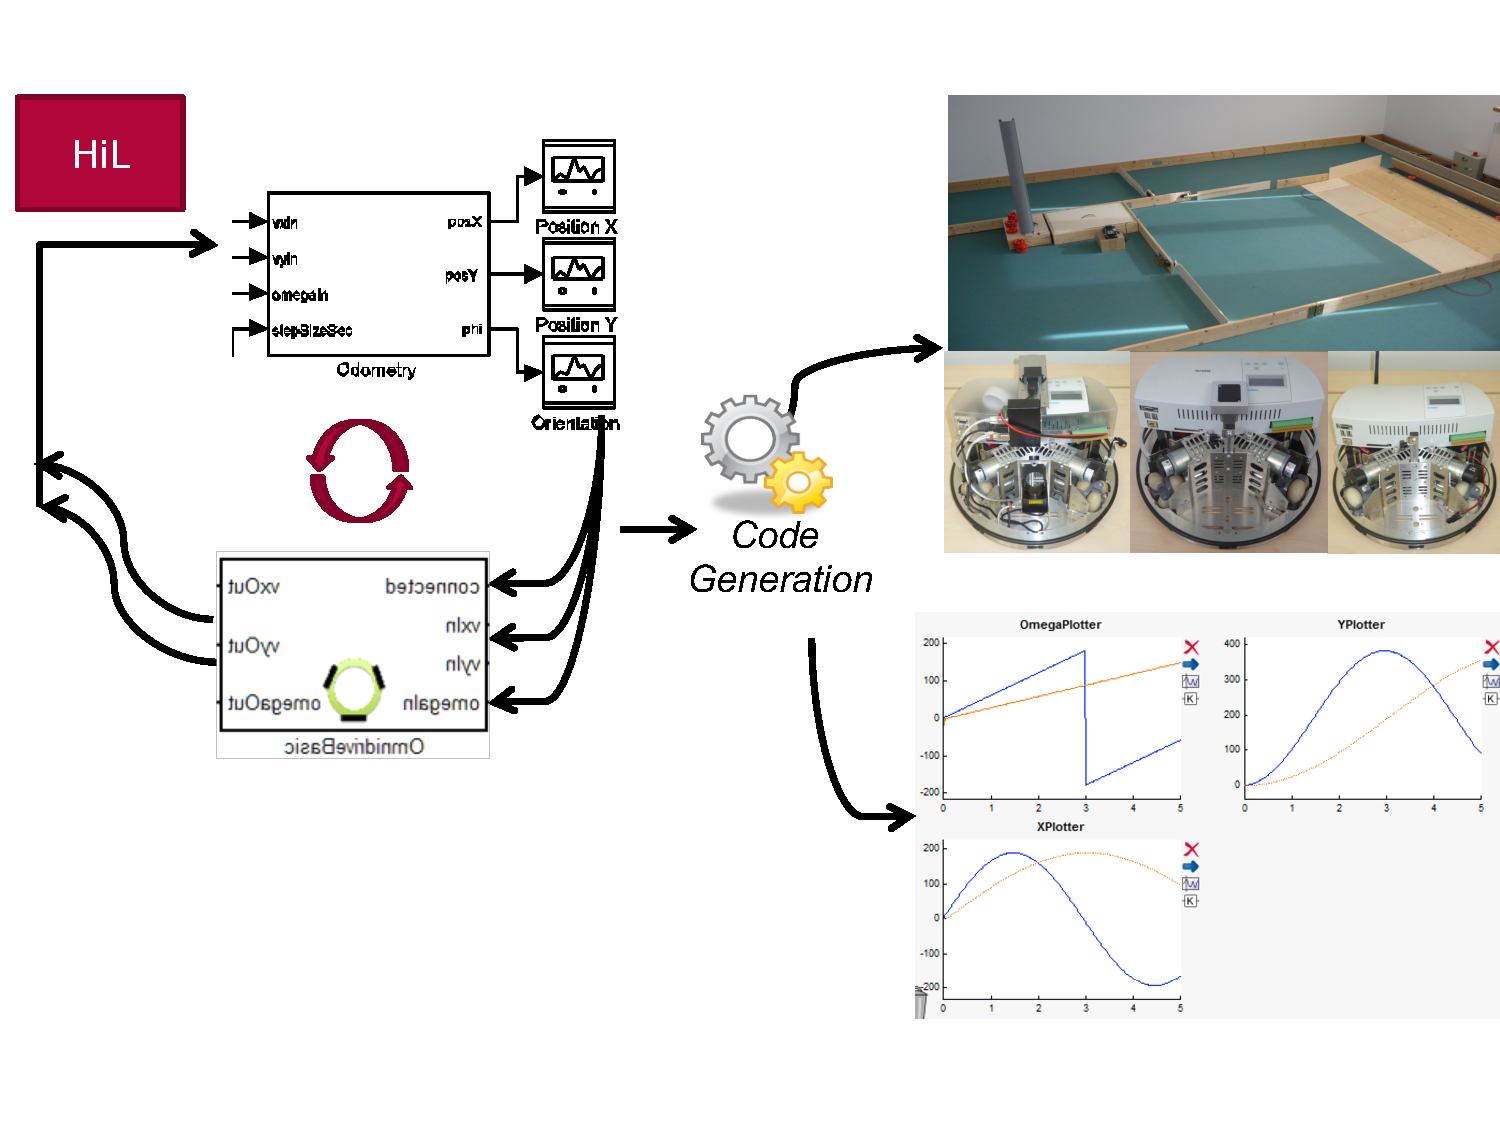
\includegraphics[scale=0.33]{figures/hil.pdf}
\caption{Overview of hardware-in-the-loop (HiL) testing in the prototyping stage of \cite{Broekman&Notenboom2003}}
\label{fig:hil}
\end{figure}


% ============================================
\subsubsubsection{Hardware in the Loop (HiL)}
%
By moving on to the lab itself, we can then also consider a \emph{hardware-in-the-loop} (HiL) simulation at the prototyping stage as sketched in Figure~\ref{fig:hil}. Besides the software that is generated or integrated, the specific characteristics of the robot hardware and lab environment and its hardware can also be experienced.

As we now employ the real hardware, we no longer ignore resp.~simplify any elements. Therefore, now real sensor values with noise, specific effects of scheduling, the impact of communication interaction and messages, and timing/memory/computation constraints\uidx{Constraint} are all considered.

% ============================================
\subsubsubsection{Hardware in the Loop (HiL) - CPS Ontology}
%
The hardware in the loop (HiL) executing the software on the robot depicted in Figure~\ref{fig:hil} ensures that the detailed control algorithm from the cyber domain is brought together with the physics as present in the robot and thus we have clearly a cyber-physical setting. 

Thus we cover the elements \CPSCyberPart from the CPS ontology for the combination of all function and the elements \CPSPhysicalPart from the CPS ontology for the whole robot.




% ============================================
\subsubsection{Pre-Production Stage}
%
In our specific setting and due to our focus on the software development, the \emph{system test} in the pre-production stage is not really different as we do not produce any system we want to sell later. In a commercial setting the robots in the prototyping, the robots in the lab would likely be equipped with more testing hardware or prototypical hardware, while in our lab only one level exists here.

The outlined methodology and tool chain adjusted from the automotive domain, provides suitable guidance due to the different focus in stages and follows where possible an MDE approach where tools and libraries are integrated such that the models drive the development. Only later the code and configuration data automatically generated from the models are employed to consider more details concerning the verification, simulation, and testing.
%
We put special focus on supporting also hard and soft real-time considerations, which are oftentimes ignored in robotic development scenarios.

\TODONOTE{ HG: add steps when considering multiple robots? }



\LATER{ HG: The links to the CPS ontology that are present in the case study are quite weak and so far only refer to the elements. Maybe we can refine them when the improved version of the CPS ontology is available? 

Right now we have:

- separation into physical and cyber elements covered by the ontology are referenced

- maybe properties of the CPS can be added?

}





% ========================================================================================
\subsection{MPM}\label{subsec:cpslab-mpm}

For the MPM ontology introduced in Chapter~\ref{ch:mpm}, we will in the following use the details of the different development steps to outline how the development is linked to MPM.

% ============================================
\subsubsection{Overview}
%


\SKIP{
\begin{figure}[!htb]
\centering
\includegraphics[width=0.8\textwidth]{figures/toolchain.pdf}
\caption{Overview of the employed tool chain (see \cite{Waetzoldt:2012pa})}
\label{fig:toolchain}
\end{figure}

An additional element depicted in Figure~\ref{fig:toolchain} is a prototype tool we developed to map AUTOSAR models to a real-time simulator from INCRON to permit detailed performance evaluation early on in parallel to SiL activities.
%
Another extension not depicted in Figure~\ref{fig:toolchain} is a link between the SysML tool TOPCASED and the dSPACE tool SystemDesk for AUTOSAR that permits to derive the software and hardware architecture in AUTOSAR from the SysML system engineering models.
%
However, to keep things simpler we omit both extensions in our detailed description and the sketches of the megamodels.

\begin{figure}[!htb]
\centering
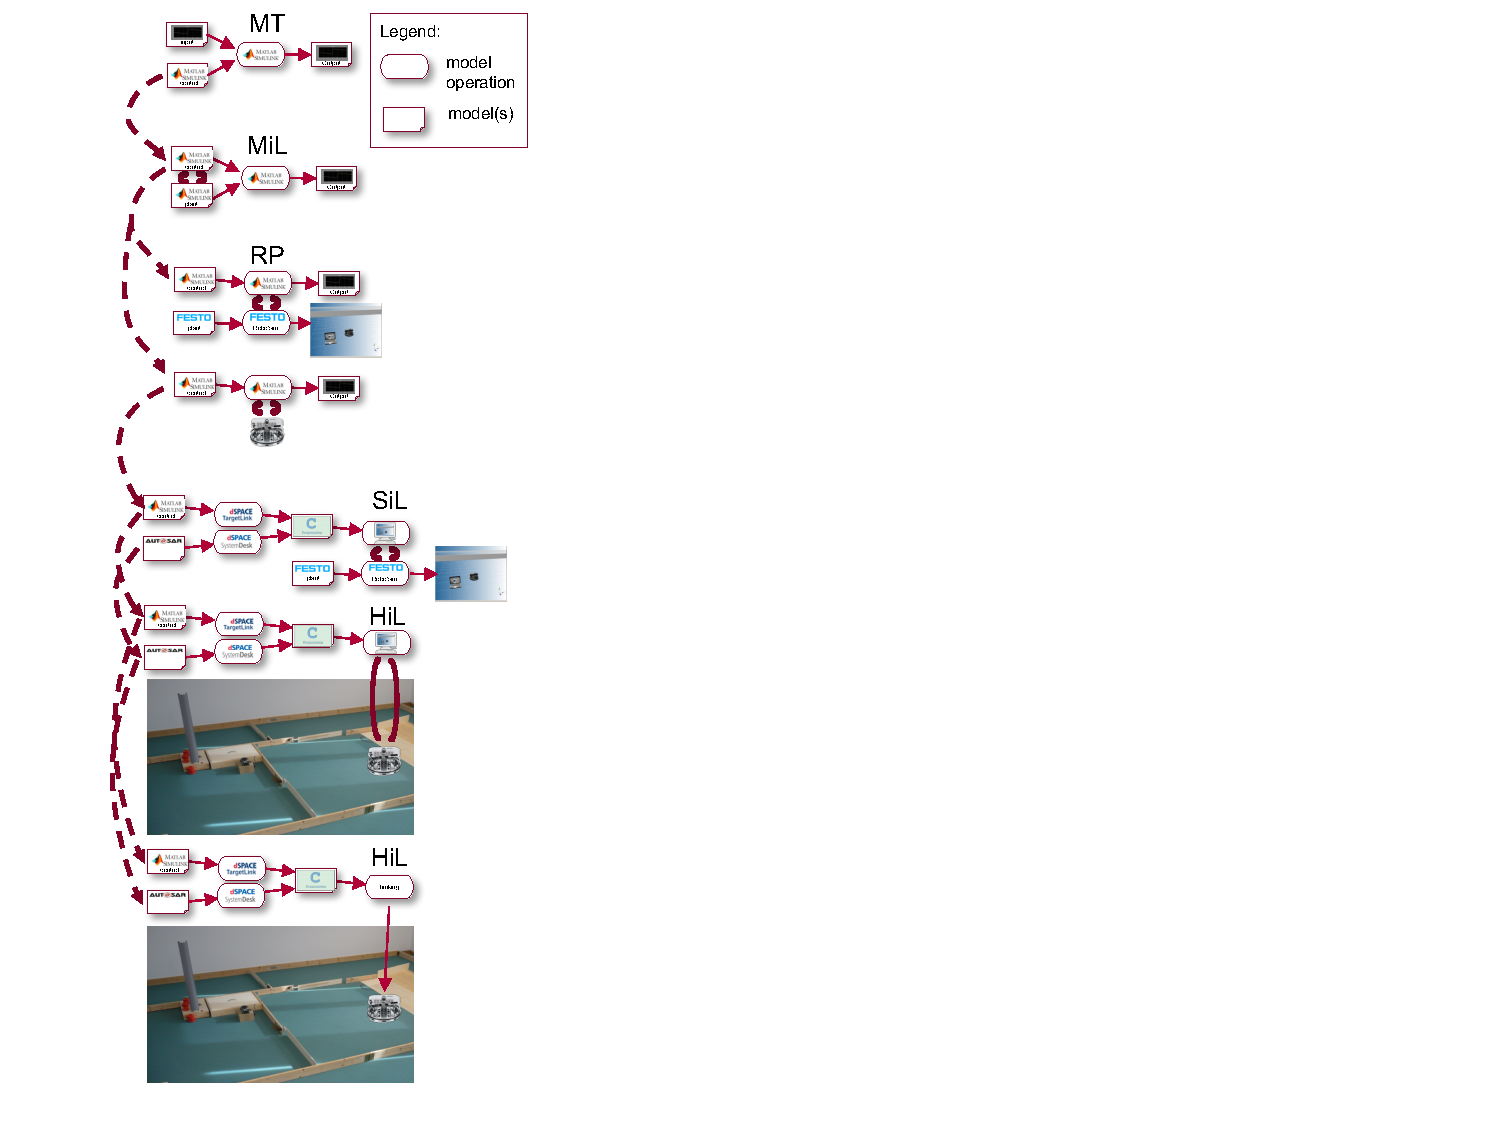
\includegraphics[scale=1.25]{figures/mm.pdf}
\caption{Sketch of the megamodel of the different stages of \cite{Broekman&Notenboom2003}}
\label{fig:mm}
\end{figure}

While several tools are employed at several stages and activities, the models developed for each of these activities are quite different as visible in the megamodel depicted in Figure~\ref{fig:mm}.

}

\begin{figure}[!htb]
\centering
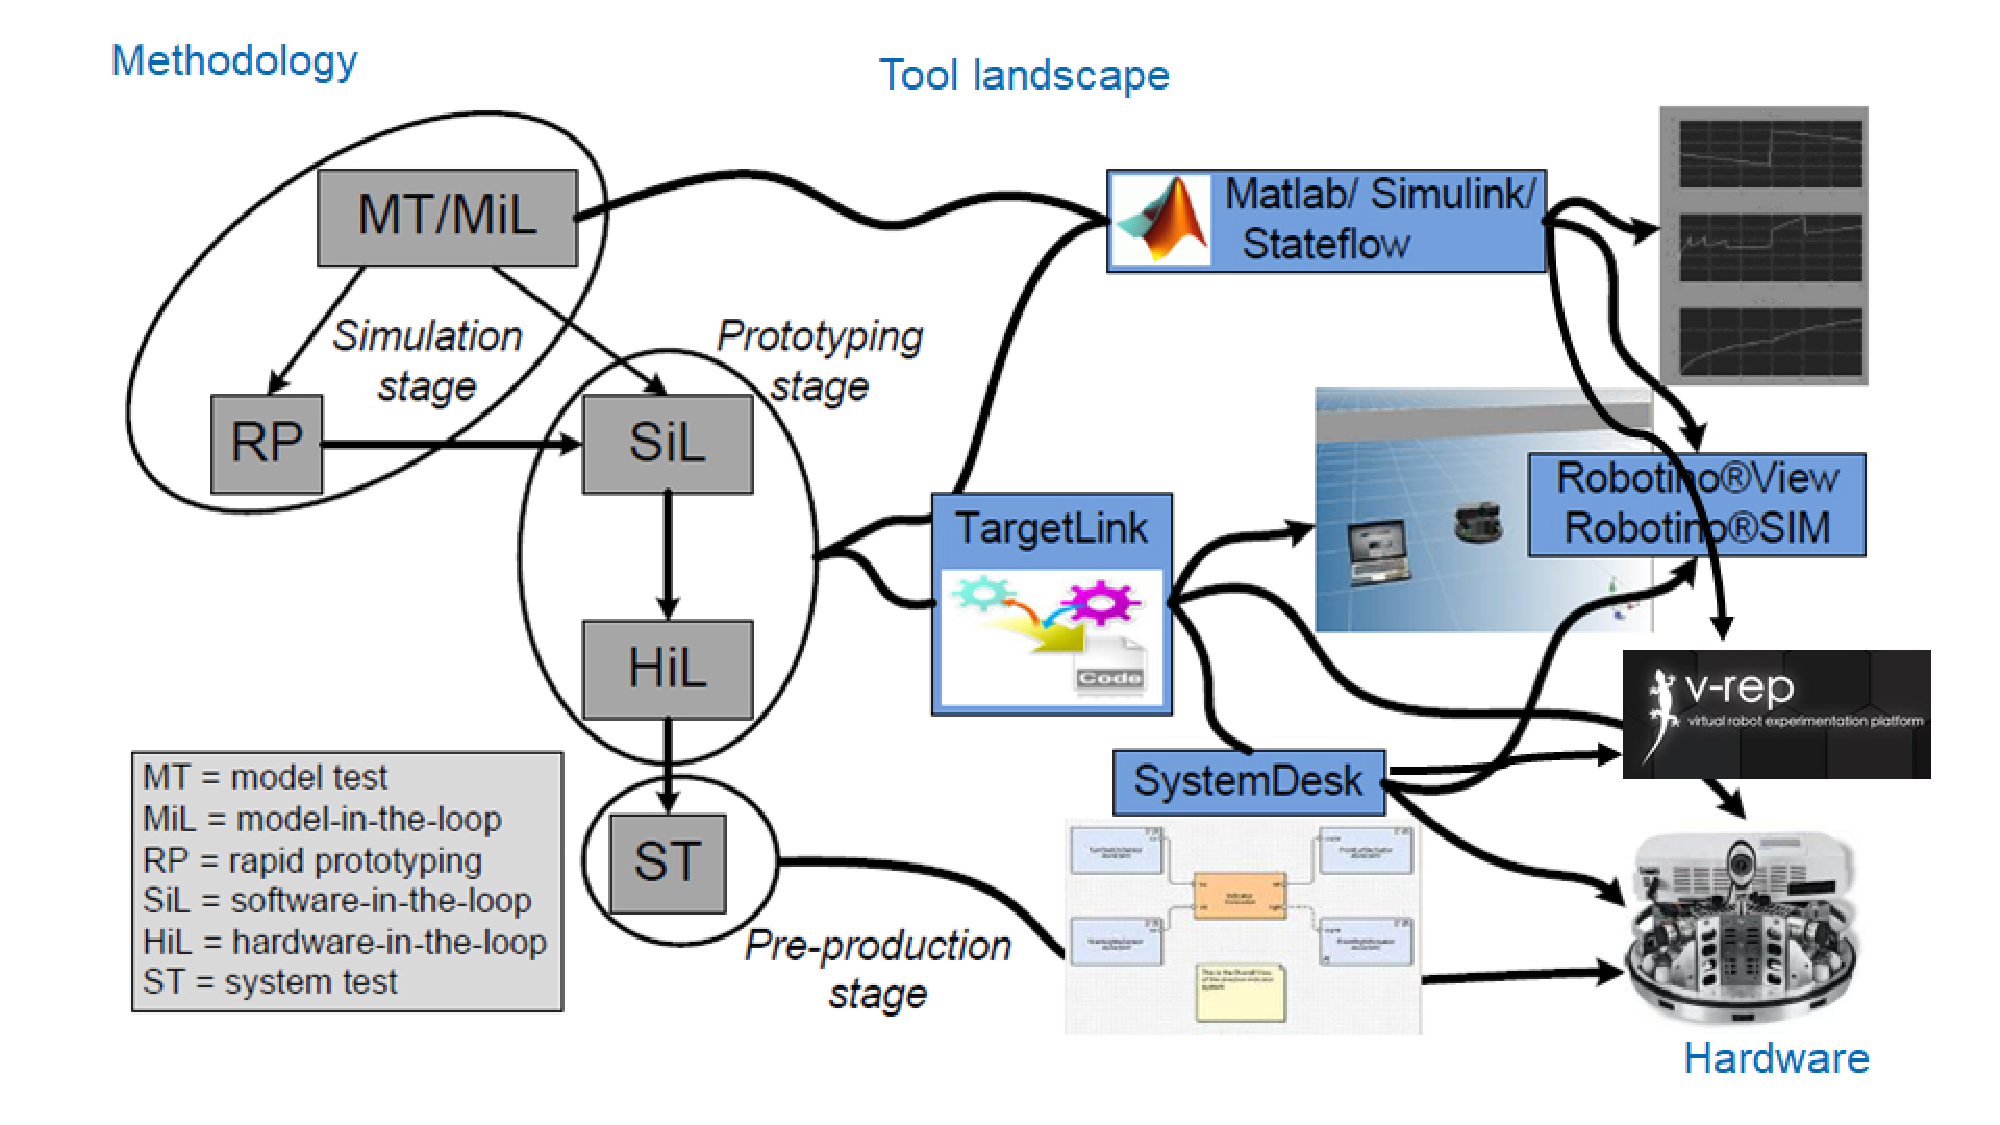
\includegraphics[width=0.9\textwidth]{figures/mm-hpi2.pdf}
\caption{Tool landscape and its relation to the development methdology}
\label{fig:MMFig2}
\end{figure}

%\todo{DB: Should that be part of the MPM section? HG: yes}
In Figure~\ref{fig:MMFig2} the tool landscape for developing the aforementioned robot CPS is depicted. It consists of
%
MATLAB/Simulink for modeling and simulation,
%
dSPACE SystemDesk for modeling software architecture, hardware configuration, and task mapping,
%
dSPACE TargetLink for code generation and
%
the FESTO Robotino-Library with the FESTO Robotino{\copyright}Sim simulator.

\begin{figure}[!htb]
\centering
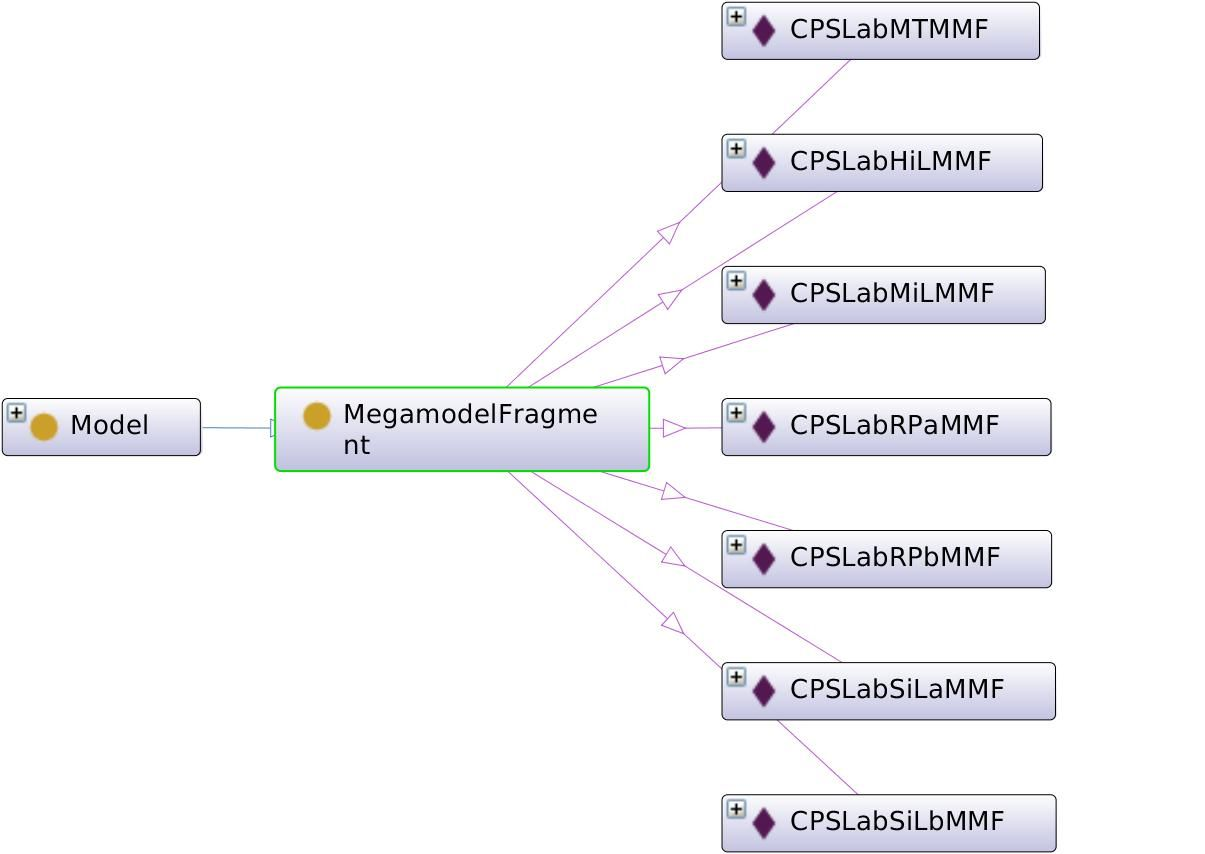
\includegraphics[scale=0.4]{figures/CPSLabMTMMF-NEW.jpeg}
\caption{All megamodel fragments\uidx{MegamodelFragment} of the \CPSLabMM megamodel\uidx{Megamodel}}
\label{fig:MegaModelFragmentsForCPSLabMM}
\end{figure}
 
%\begin{figure}[!htb]
\begin{figure}[p]
\centering
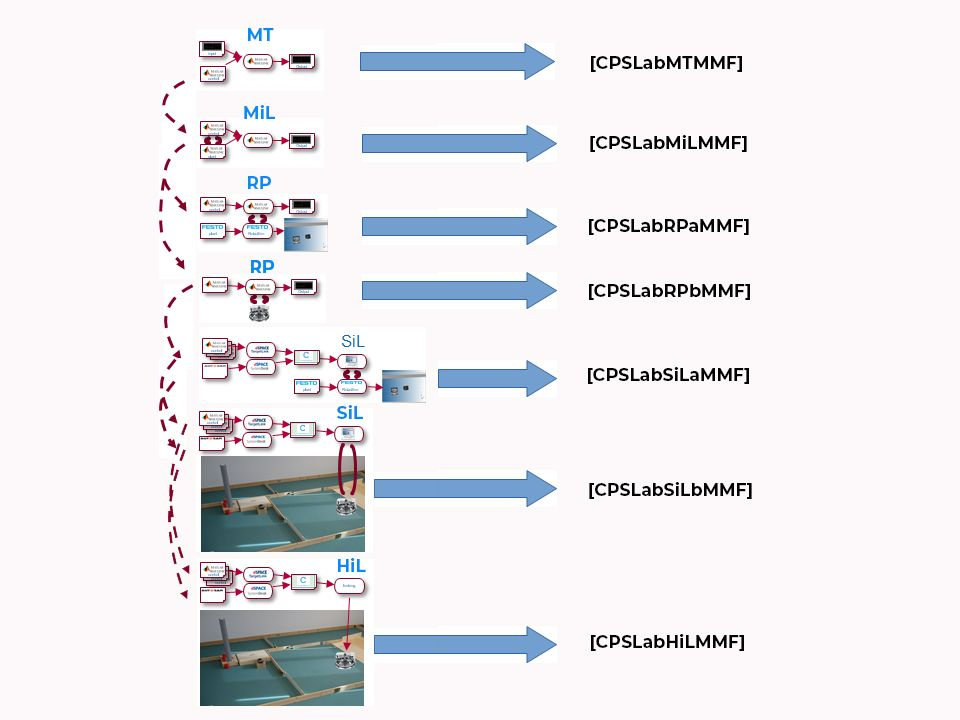
\includegraphics[scale=0.6]{figures/slide-fig.jpg}
\caption{Overview over the megamodel fragments of the CPSLab megamodel\uidx{Megamodel} and how the models are related (dashed arrows)}
\label{fig:MMFig10}
\end{figure}

\TODOINLINE[SB]{ HG: Please add names of the megamodelfragments to the graphics of Figure~\ref{fig:MMFig10}. We should use the names defined int the subsequent figures which show the fragments of the megamodel in our PPT-slide notation MT (see Figure \ref{fig:CPSLabMTMMF} for a case where MT (for Model Test) and  \CPSLabMTMMF (as the name of the related MegaModelFragmeent) should be added. In most case the short name (e.g., SiL) has been already added. }

\TODOINLINE[SB]{ HG: Please remove the methodology part in Figure~\ref{fig:MMFig10} (large red boxes with MT, MiL, RP, ... as this has been shown on the former figure already. Please ove the legend to the the remaining graphicasl elements.}

On overview about the stages and activities with an emphasis on models, tools, and multi-paradigm modeling is depicted in Figure~\ref{fig:MMFig10}.

In the following, we outline to which elements of the MPM ontology of Chapter~\ref{ch:mpm} the elements of the megamodel\uidx{Megamodel} refer and which megamodel fragments\uidx{MegamodelFragment} cover the scenarios introduced in the last subsection.

\LATER{ HG: Is an introduction to the notation required? Do we have to explain the links to the MPM ontology concepts here?}

\subsubsubsubsection{Formalism, Languages, Models, and Tools}

\LATER[Formalism]{
\item Formalism
    \begin{itemize}
        \item Automated Based Formalism: Abstract state machine, Cellular automata, Input/Output Automata, Label transitions systems, Timed transitions systems
        \item Automated Based Formalism:: Hybrid Automata: Hybrid Automata, Hybrid Input/Output automata, Linear hybrid automata, Non-Linear Hybrid Automata, Stocastics hybrid automata 
        \item Automated Based Formalism:: Hybrid Automata:: Timed Automata: , Stockists timed automata, Timed Automata, PTS.
        \item Flow Based Formalism: Data Flow, State Flow, Data Flow timed, HyFlow.
        \item Logic Based Formalism: First order logic, Linear temporal logic, CTL, Temporal Logic 
        \item Petri net based formalism: High Level Petri net, Petri net, Petri net with priyority, Petri net with time, dPN, Timed Petri net
        
    \end{itemize}
}

\begin{itemize}
    \item Used Language and Models
    \begin{itemize}
        \item \MATLABSimulinkLanguage: \CPSLabControlModel, \CPSLabPlantModel
        \item \FESTORobotinoSimLanguage: \CPSLabRobotModel
        \item \AUTOSARLanguage: \CPSLabSystemModel
    \end{itemize}
    \item MegaModel\uidx{Megamodel}
    \begin{itemize}
        \item MegaModel: \CPSLabMM
        \item MegaModelFragments\uidx{MegamodelFragment}: \CPSLabMTMMF, \CPSLabMiLMMF, \CPSLabRPaMMF, \CPSLabRPbMMF, \CPSLabSiLaMMF, \CPSLabSiLbMMF, \CPSLabHiLMMF
        \item ModelRealtions: (see detailed definition of the megamodel fragments)
    \end{itemize}
    \item Tool
    \begin{itemize}
        \item SimulationTool: \MATLABSimulinkSimulator
        \item TransformationTool: \dSPACETargetLink
        \item ModelingTool: \dSPACESystemDesk
        \item SimulationTool: \FESTORobotinoSim
        \item VisualizationTool: \FESTORobotinoView
        \item ExecutionTool: \DesktopExecution
        \item ExecutionTool: \RobotExecutionRemote
        \item ExecutionTool: \RobotExecutionLocal \LATER{ HG: check tool types!}
    \end{itemize}
\end{itemize}

\DONE[HG]{ HG: please add scheme for MPM ontology use here! }
\DONE[SB]{ HG: please model scheme for MPM ontology presented here with Protege! }
\DONE[SB]{ HG: please add figure showing the used MPM ontology elements here! }



The added elements for the CPSLab ontology outlined in the text are depicted also in Figure~\ref{fig:MegaModelFragmentsForCPSLabMM}.

% ============================================
\subsubsection{Simulation Stage}
%
In the simulation stage we have two development activities: model test and model-in-the loop.
%
In the following, we will outline how they can be captured with mega-model fragments consisting of model instances and tool applications.





% =========================================
\subsubsubsection{Model Test}
%
The model test introduced in Figure~\ref{fig:mt}, is rather trivial as it only employ a single model of the planned control algorithm plus some auxiliary models for test inputs. Then, as depicted in Figure~\ref{fig:MMFig3} the model of the control algorithm is simulated by employing the test inputs.

\begin{figure}[!htb]
\centering
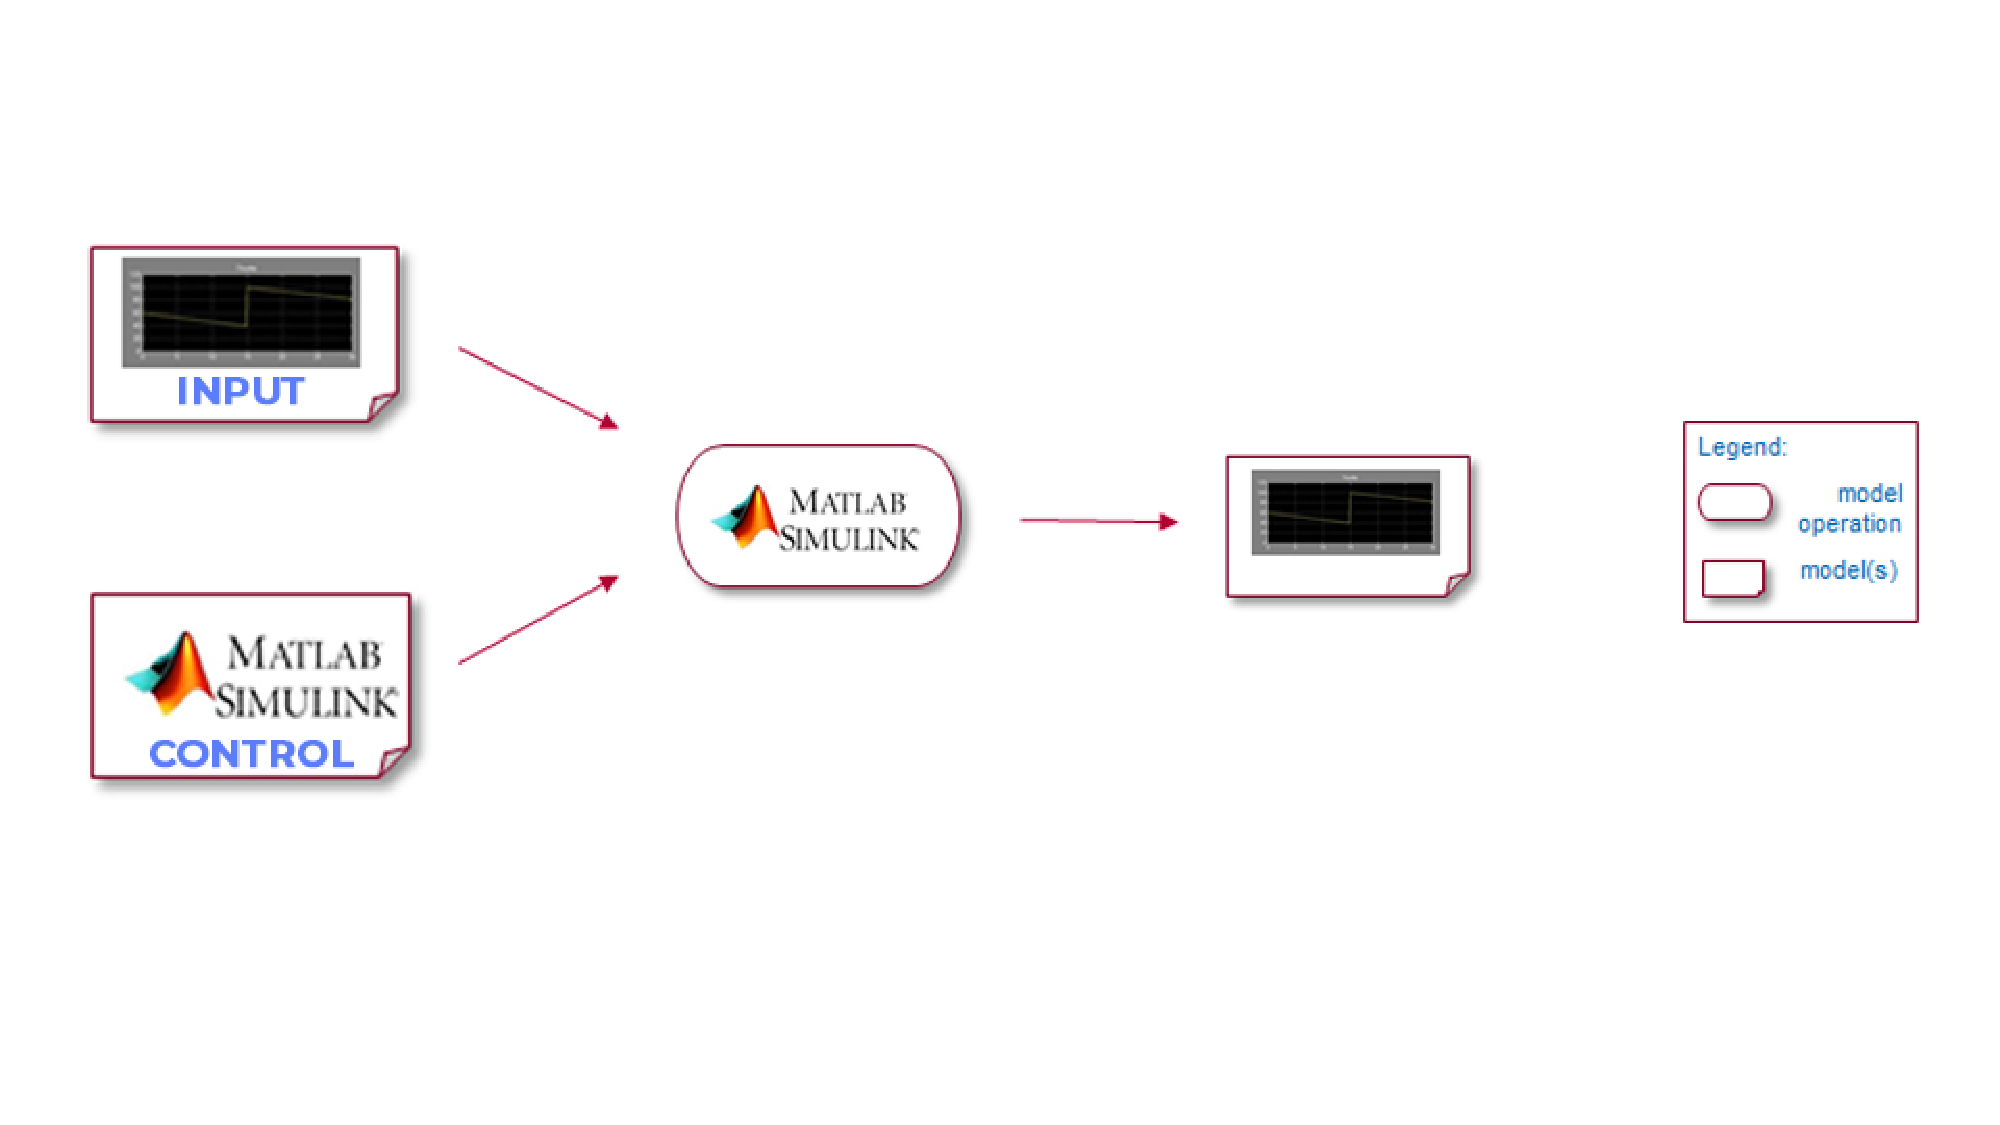
\includegraphics[scale=0.33]{figures/mm-hpi3.pdf}
\caption{Model Test}
\label{fig:MMFig3}
\vspace{-0.2in}
\end{figure}

% =========================================
\subsubsubsection{Model Test - MPM Ontology}
%
%
\subsubsubsubsection{MegaModel Fragment \CPSLabMTMMF}

\begin{itemize}
    \item MegaModelFragment: \CPSLabMTMMF
    \begin{itemize}
        \item Model(s): \CPSLabControlModel
    \end{itemize}
\end{itemize}

\subsubsubsubsection{Tools / Models Operations of \CPSLabMiLMMF}

\begin{itemize}
    \item \uidxp{ModelOperation}: One Shot Simulation
    \begin{itemize}
        \item Input Model(s): \CPSLabControlModel, Input data (entered with \MATLABSimulinkSimulator)
        \item Output Model(s): Output data (visualized with \MATLABSimulinkSimulator)
        \item Employed Tool: \MATLABSimulinkSimulator \COMMENT{\tiny THIS ENTRY IS NOT COVERED BY THE ONTOLOGY SO FAR}
    \end{itemize}
\end{itemize}

\LATER{
\subsubsubsubsection{Development Process}
 
FREE TEXT CAPTURING THE ORDERING
}

\DONE[HG]{ HG: please add scheme for MPM ontology use here! }
\DONE[SB]{ HG: please model scheme for MPM ontology presented here with Protege! }
\DONE[SB]{ HG: please add figure showing the used MPM ontology elements here! }

\begin{figure}[!htb]
\centering
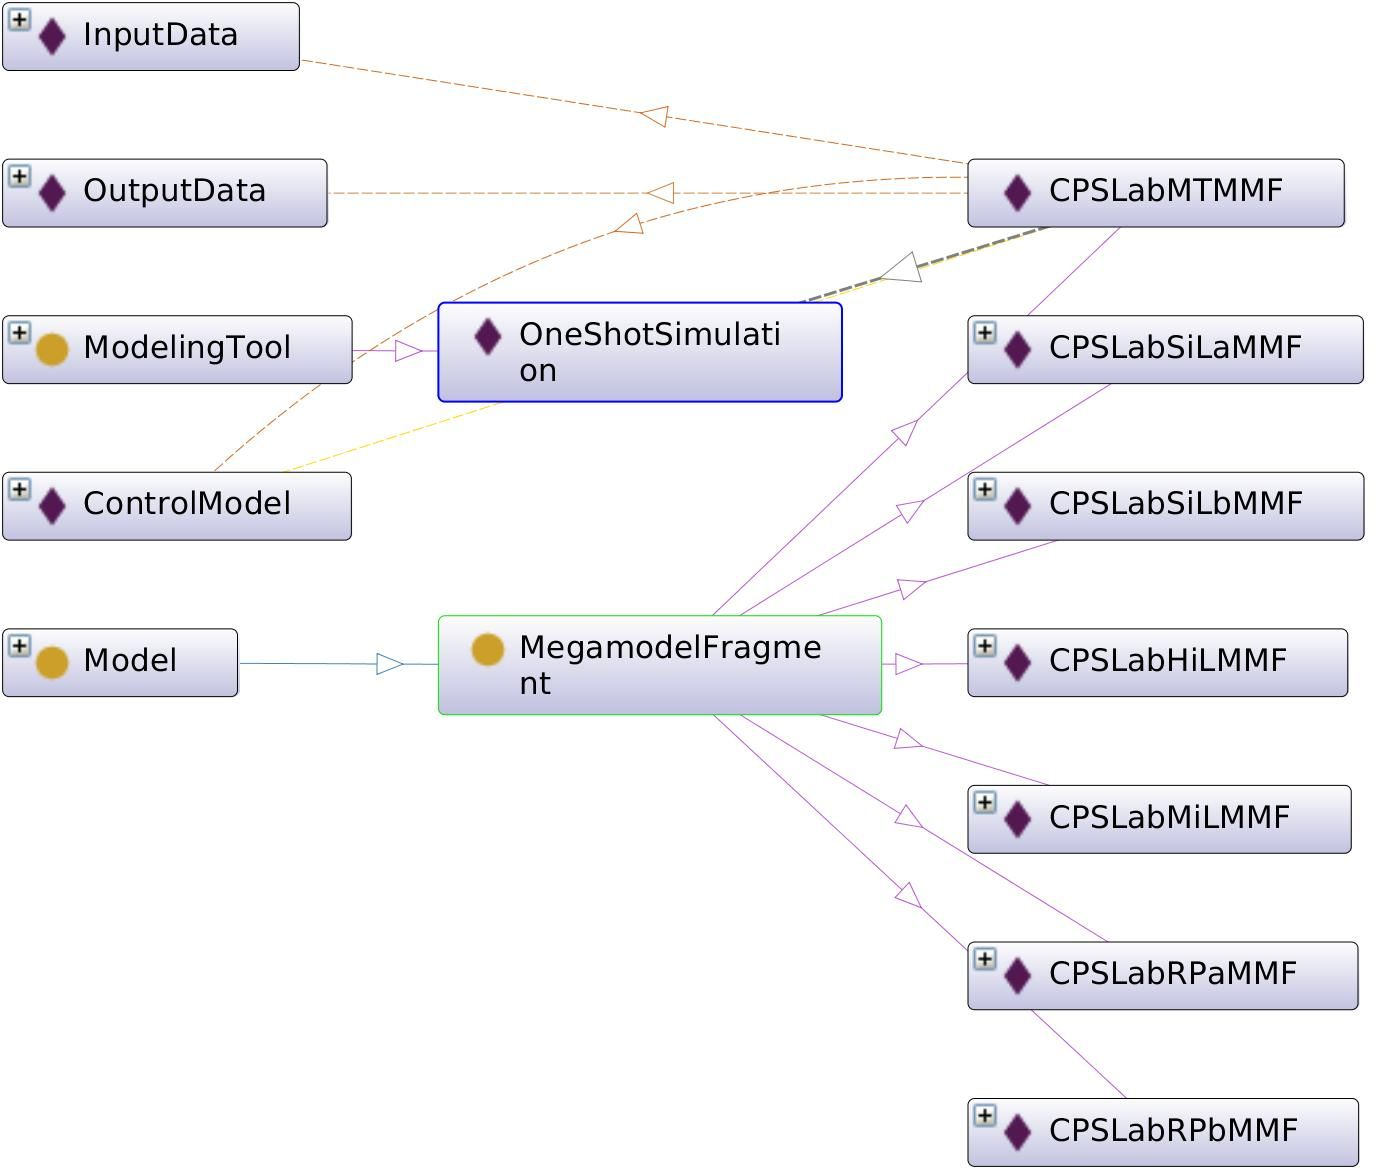
\includegraphics[scale=0.3]{figures/CPSLabMTMMF-NEW-1.jpeg}
\caption{Part of the ontology for the megamodel fragment\uidx{MegamodelFragment} \CPSLabMTMMF covering the Model Test activity\uidx{Activity}}
\label{fig:CPSLabMTMMF}
\end{figure}

In Figure~\ref{fig:CPSLabMTMMF}, the added MegaModel Fragment \CPSLabMTMMF and its elements for the CPSLab ontology outlined in the text are presented.

% =========================================
\subsubsubsection{Model-in-the-Loop}
%
In contrast to model test, model-in-the-loop simulation as introduced in Figure~\ref{fig:mil} employed besides a model of the control algorithm also a model of the plant and uses as depicted in Figure~\ref{fig:MMFig4} simulation to explore how well both fit together.

\begin{figure}[!htb]
\centering
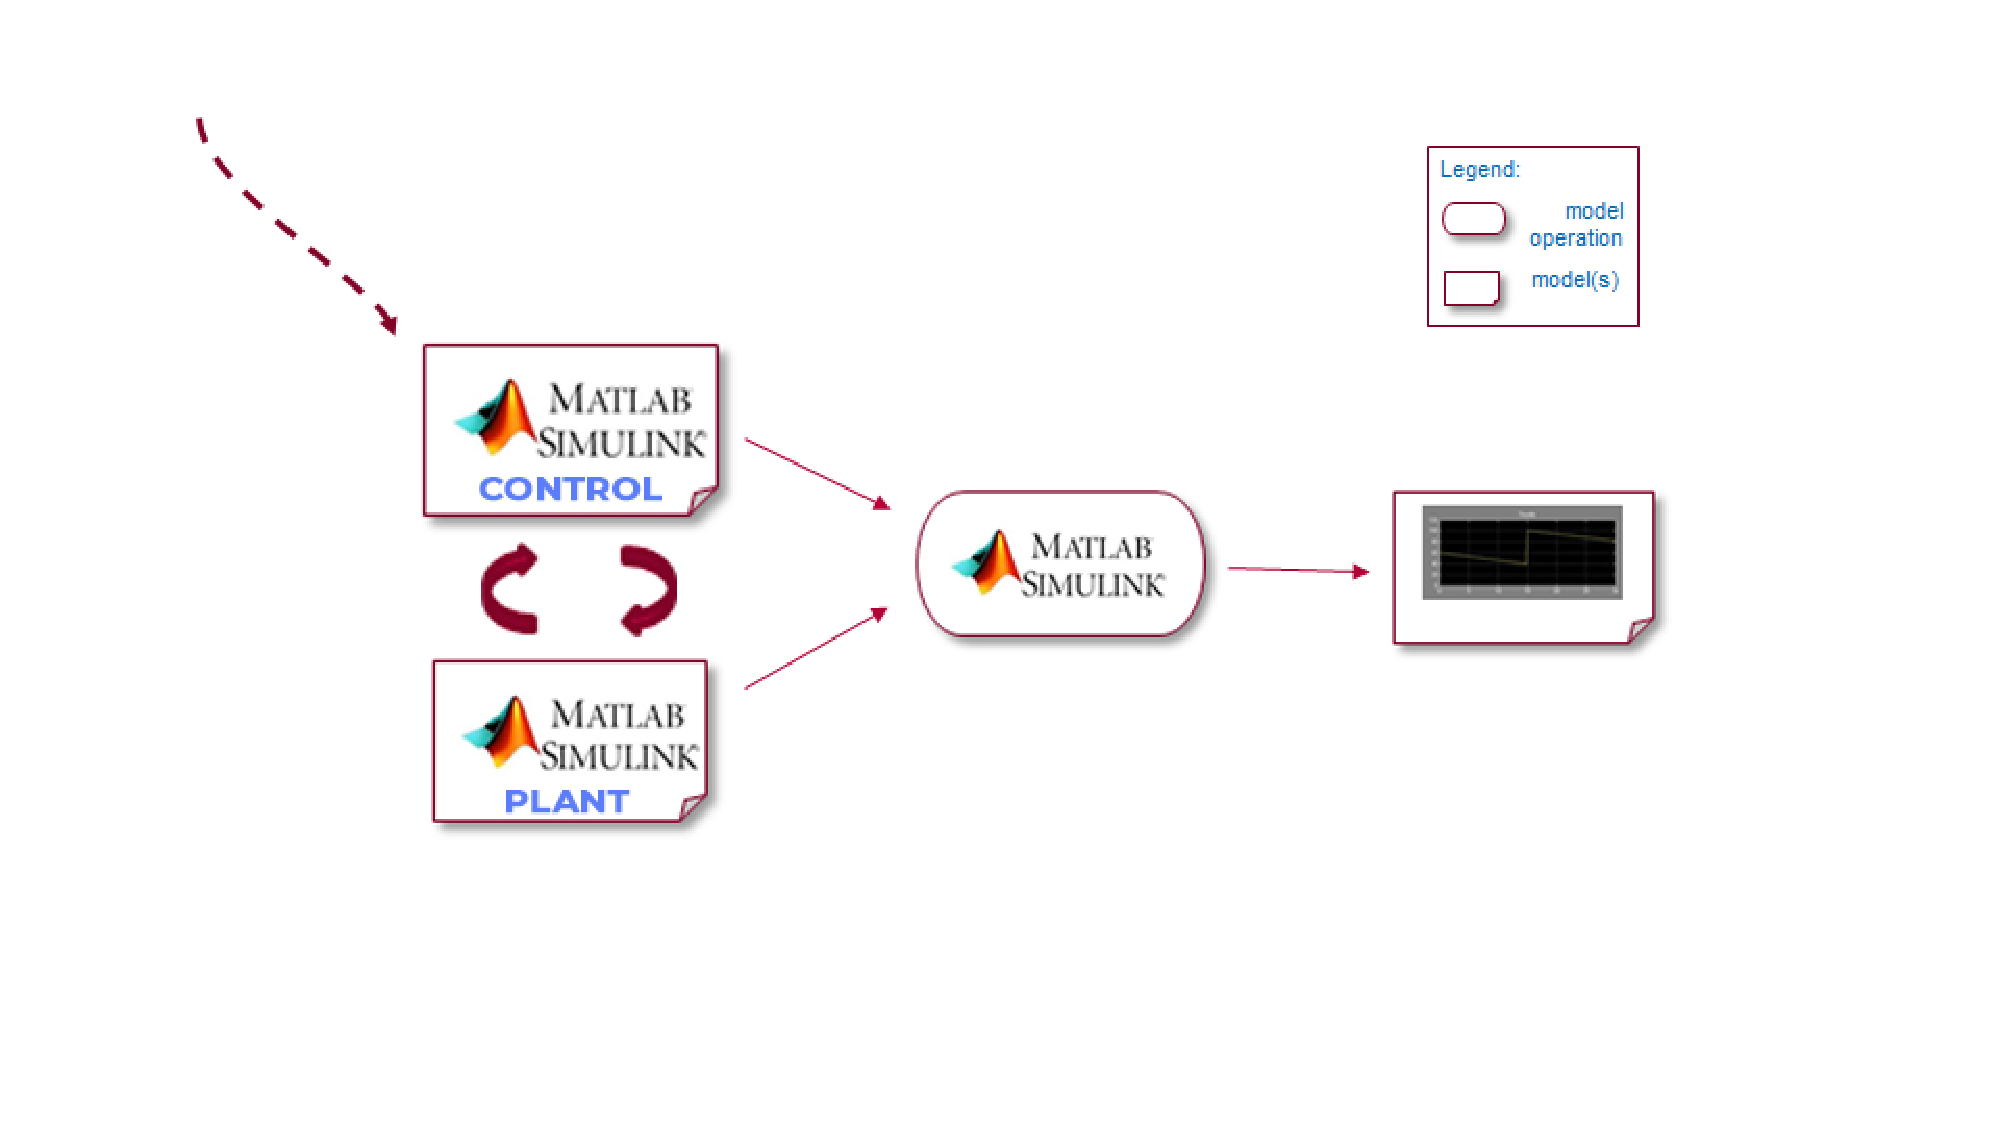
\includegraphics[scale=0.33]{figures/mm-hpi4.pdf}
\caption{Model in the Loop}
\label{fig:MMFig4}
\end{figure}

% =========================================
\subsubsubsection{Model-in-the-Loop - MPM Ontology}
%
\subsubsubsubsection{MegaModel Fragment \CPSLabMiLMMF}

\begin{itemize}
    \item MegaModelFragment: \CPSLabMiLMMF
    \begin{itemize}
        \item Model(s): \CPSLabControlModel, \CPSLabPlantModel
    \end{itemize}
\end{itemize}

\subsubsubsubsection{Tools / Models Operations of \CPSLabMiLMMF}

\begin{itemize}
    \item \uidxp{ModelOperation}: Model-in-the-Loop Simulation
    \begin{itemize}
        \item Input Model(s): \CPSLabControlModel, \CPSLabPlantModel
        \item Output Model(s): Output data (visualized with \MATLABSimulinkSimulator)
        \item Employed Tool: \MATLABSimulinkSimulator \COMMENT{\tiny THIS ENTRY IS NOT COVERED BY THE ONTOLOGY SO FAR}
    \end{itemize}
\end{itemize}

\LATER{
\subsubsubsubsection{Development Process}
 
FREE TEXT CAPTURING THE ORDERING
}

\DONE[HG]{ HG: please add scheme for MPM ontology use here! }
\DONE[SB]{ HG: please model scheme for MPM ontology presented here with Protege! }
\DONE[SB]{ HG: please add figure showing the used MPM ontology elements here! }

\begin{figure}[!htb]
\centering
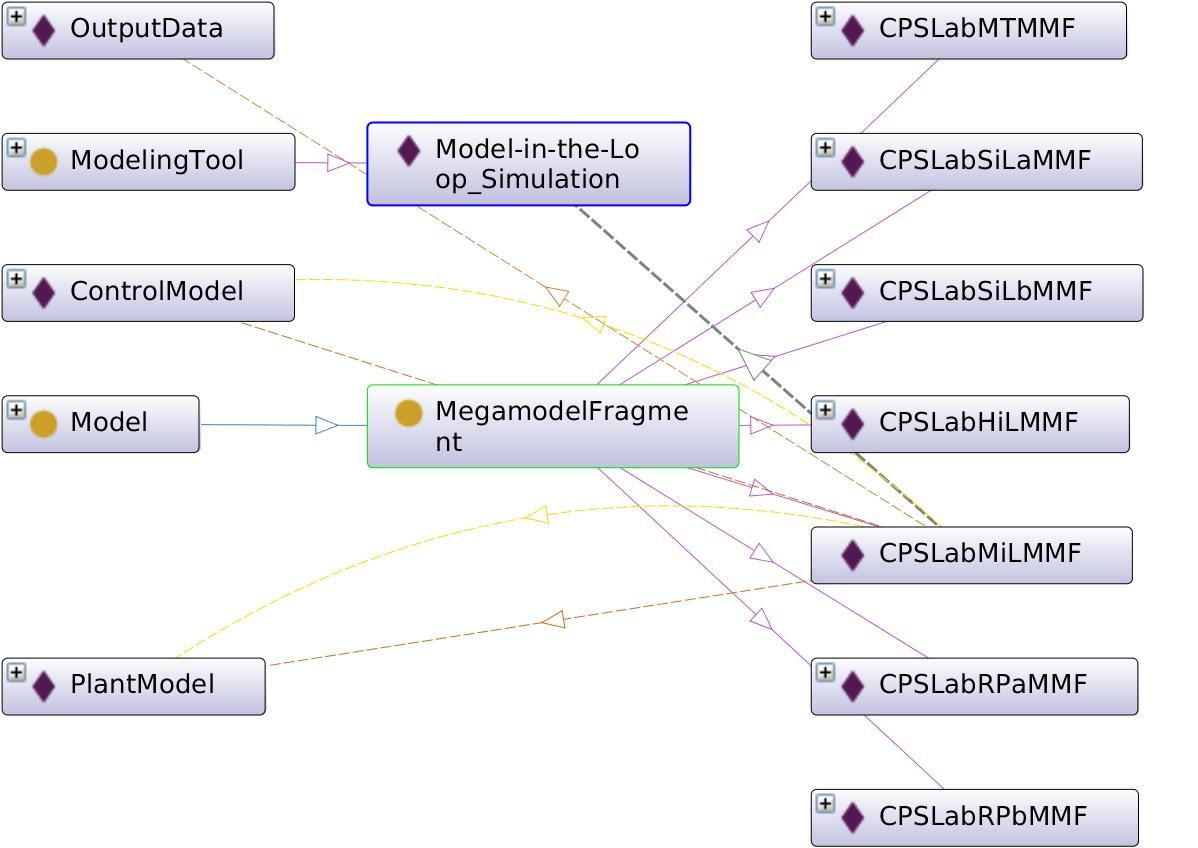
\includegraphics[scale=0.38]{figures/CPSLabMilMMF.jpg}
\caption{Part of the ontology for the MegaModelFragment\uidx{MegamodelFragment} \CPSLabMiLMMF covering Model-in-the-Loop (MiL)}
\label{fig:CPSLabMilMMF}
\end{figure}

The added MegaModel Fragment\uidx{MegamodelFragment} \CPSLabMiLMMF and its elements for the CPSLab ontology outlined in the text are depicted also in Figure~\ref{fig:CPSLabMilMMF}.

% =========================================
\subsubsubsection{Rapid Prototyping}
%
The rapid prototyping as introduced in Figure~\ref{fig:rp} is supported in two forms.
%
At first rapid prototyping can be done employing a sophisticated simulator for the robot as depicted in Figure~\ref{fig:MMFig5}. While not necessary exposing the control algorithm to physical reality as far as captured by the sophisticated model of the robot, the simulator already capture much more details than the plan model while still allowing to analyze the behavior much easier then in the case of using the real robot.

\begin{figure}[!htb]
\centering
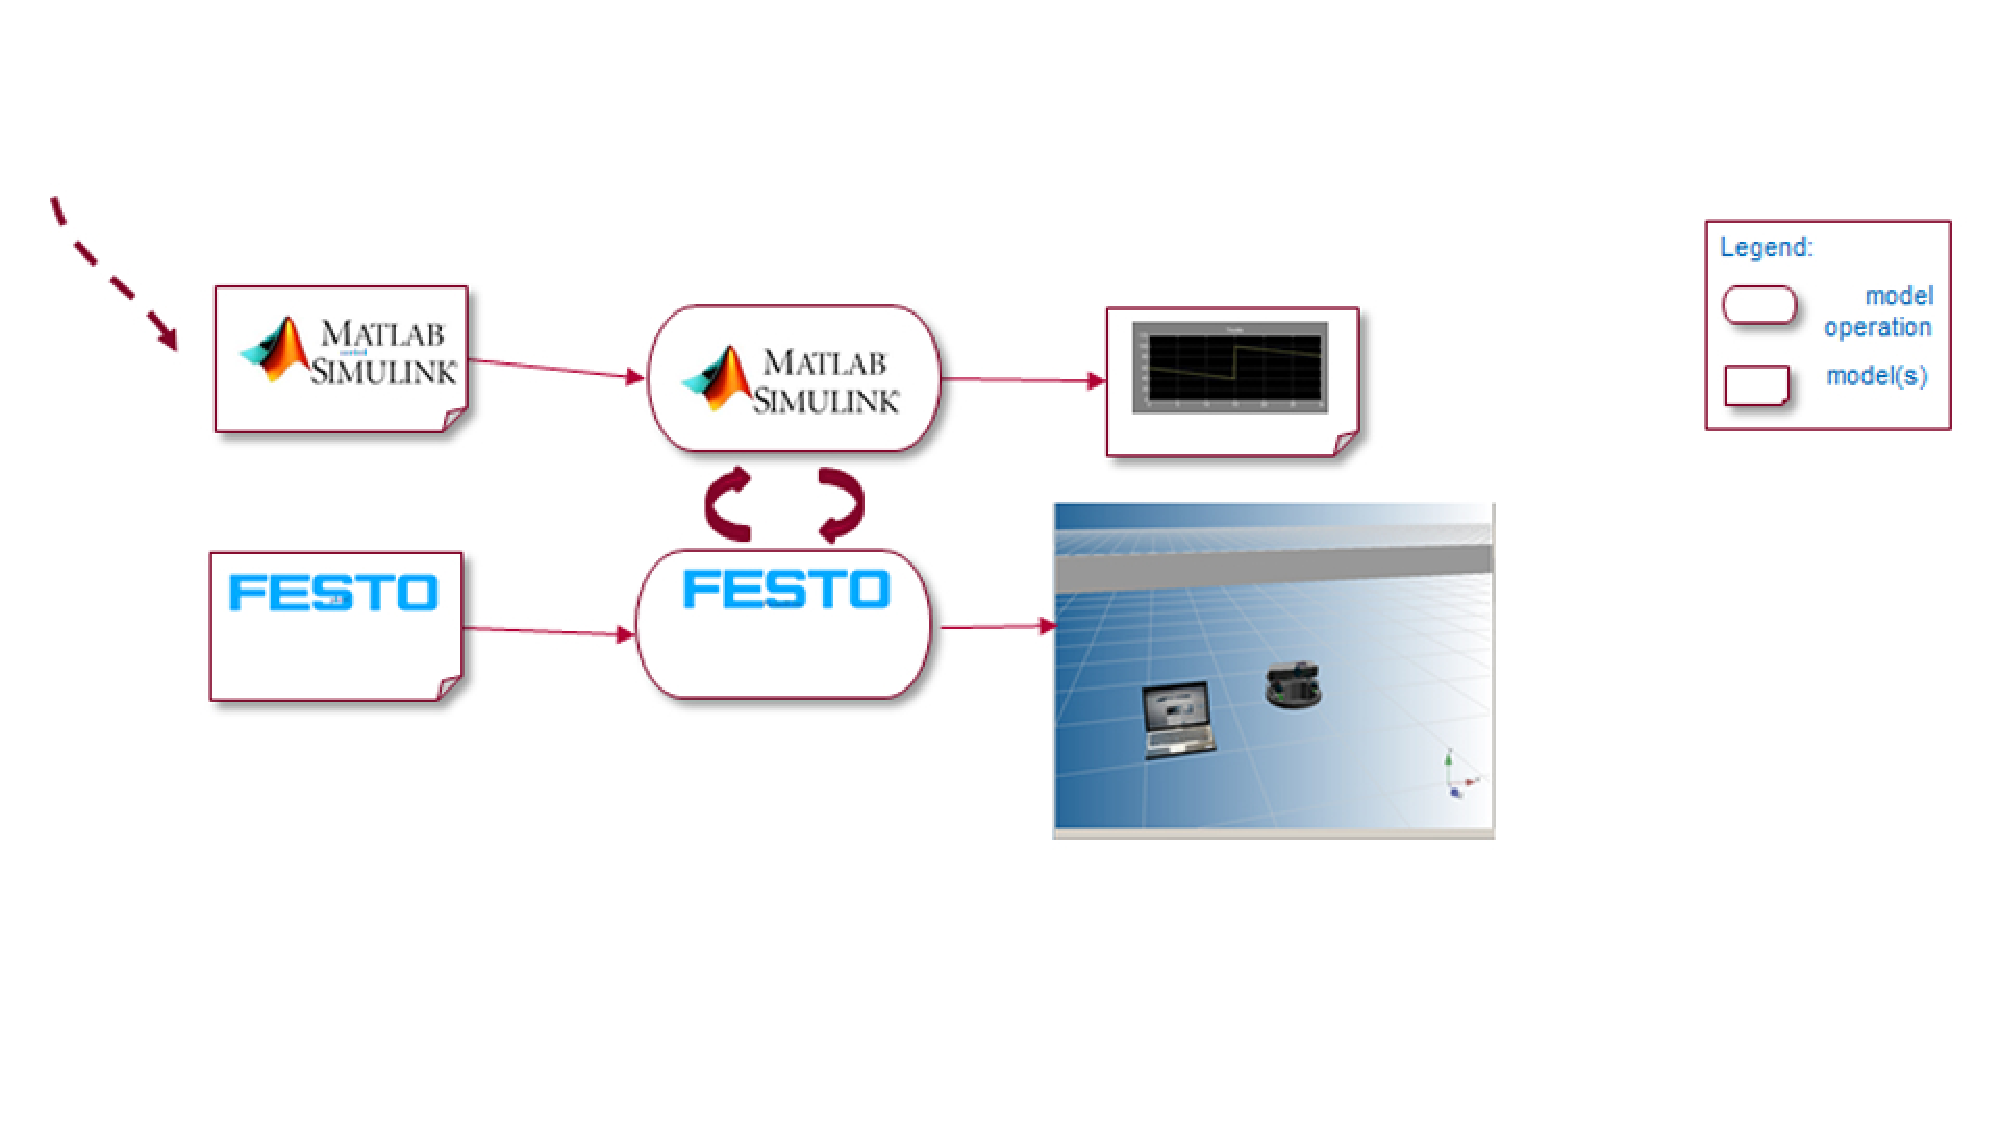
\includegraphics[scale=0.4]{figures/mm-hpi5.pdf}
\caption{Rapid Prototyping (RP) with a detailed robot simulation}
\label{fig:MMFig5}
\end{figure}

The second case depicted in Figure~\ref{fig:MMFig6} connects the abstract control algorithm with the real robot and therefore expose the algorithm to all physical effects. However, analysis might be difficult as running the algorithm against the robot is less easy to analyze then when running it against a simulator.

\begin{figure}[!htb]
\centering
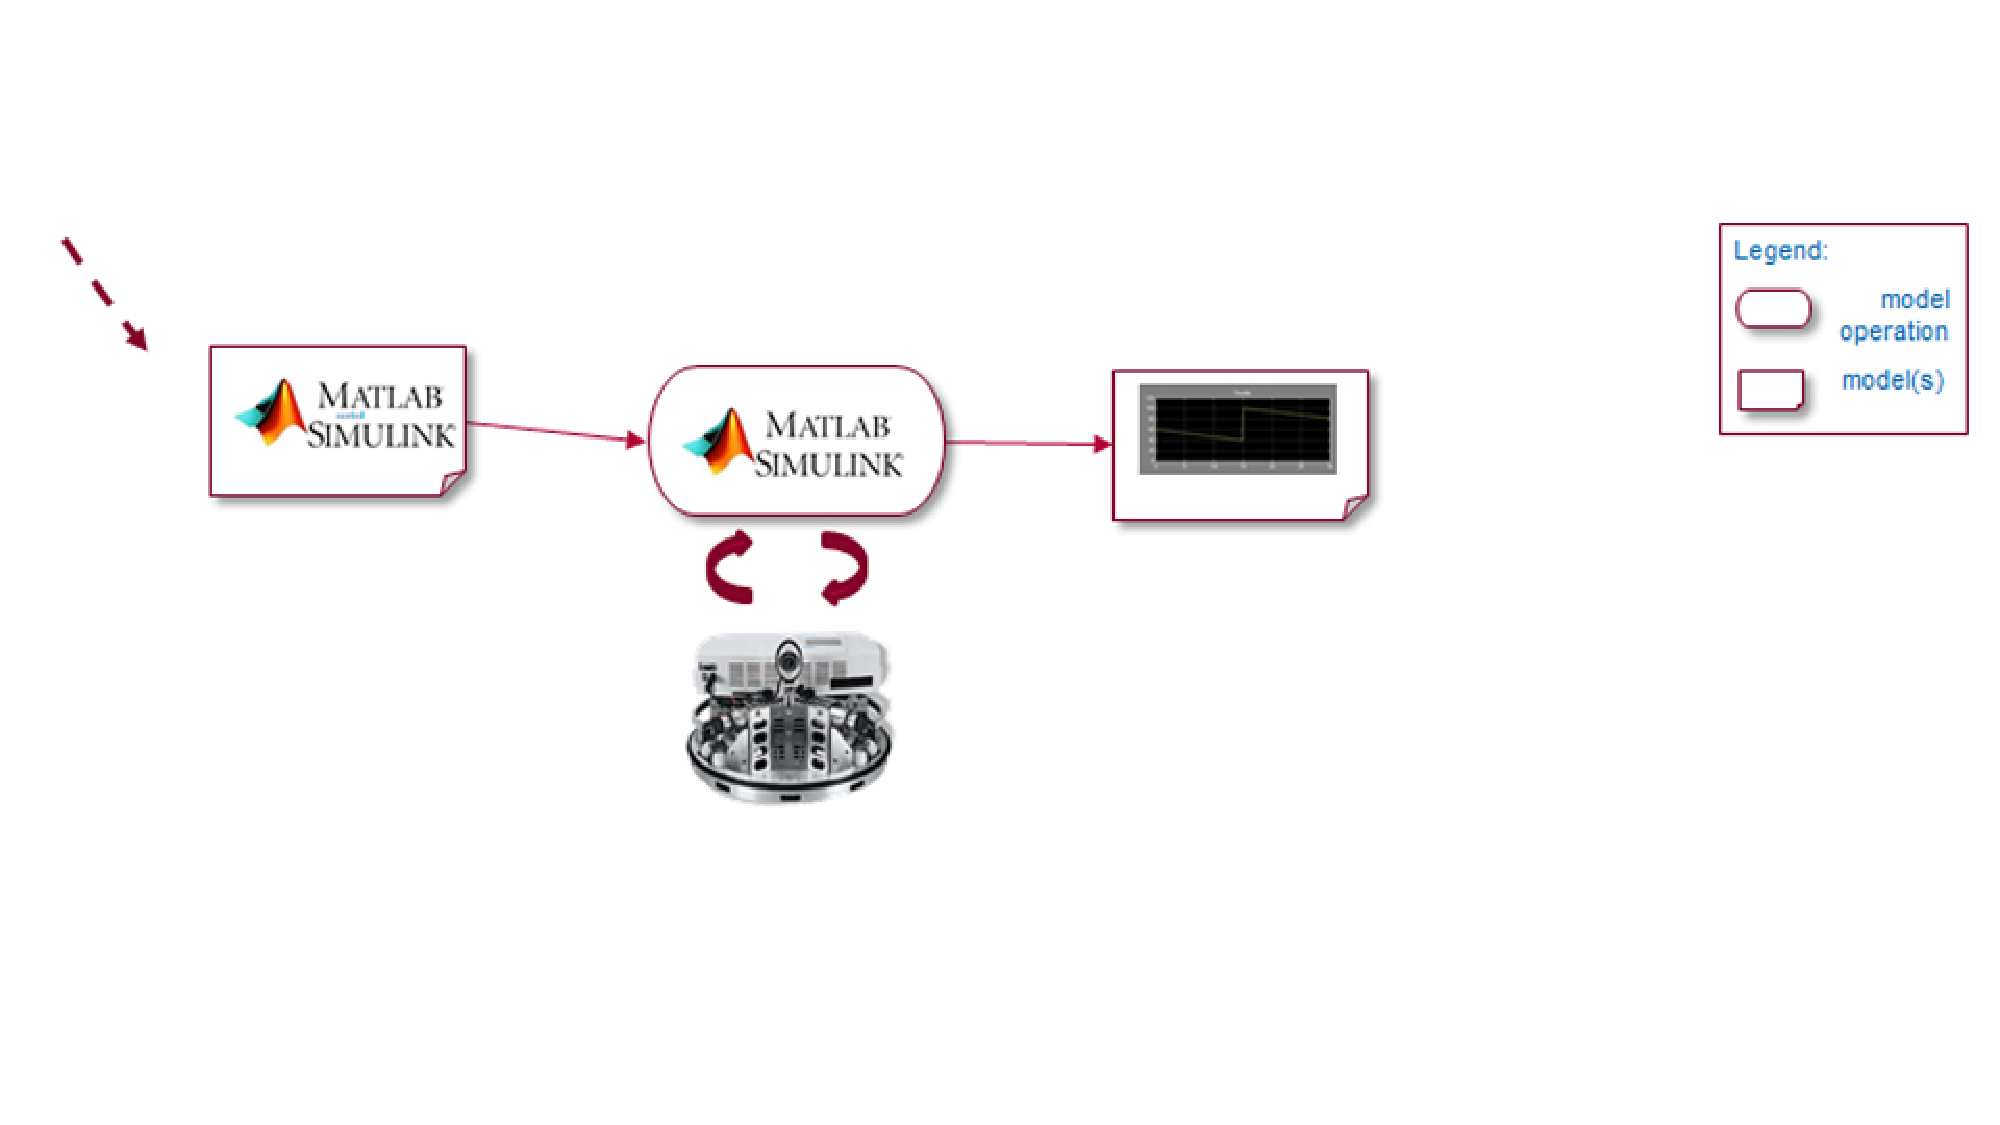
\includegraphics[scale=0.33]{figures/mm-hpi6.pdf}
\caption{Rapid Prototyping (RP) with a remote controlled robot}
\label{fig:MMFig6}
\end{figure}

% =========================================
\subsubsubsection{Rapid Prototyping - MPM Ontology}
%
%
\subsubsubsubsection{MegaModel Fragment \CPSLabRPaMMF}

\begin{itemize}
    \item MegaModelFragment: \CPSLabRPaMMF
    \begin{itemize}
        \item Model(s): \CPSLabControlModel, \CPSLabRobotModel
    \end{itemize}
\end{itemize}

\subsubsubsubsection{Tools / Models Operations of \CPSLabRPaMMF}

\begin{itemize}
    \item ModelOperation: Rapid Prototyping with Robot Simulation
    \begin{itemize}
        \item Input Model(s): \CPSLabControlModel, \CPSLabRobotModel
        \item Output Model(s): Output data (visualized with \MATLABSimulinkSimulator and/or \FESTORobotinoView)
        \item Employed Tool: \MATLABSimulinkSimulator, \FESTORobotinoSim \COMMENT{\tiny THIS ENTRY IS NOT COVERED BY THE ONTOLOGY SO FAR}
    \end{itemize}
\end{itemize}


\begin{figure}[!htb]
\centering
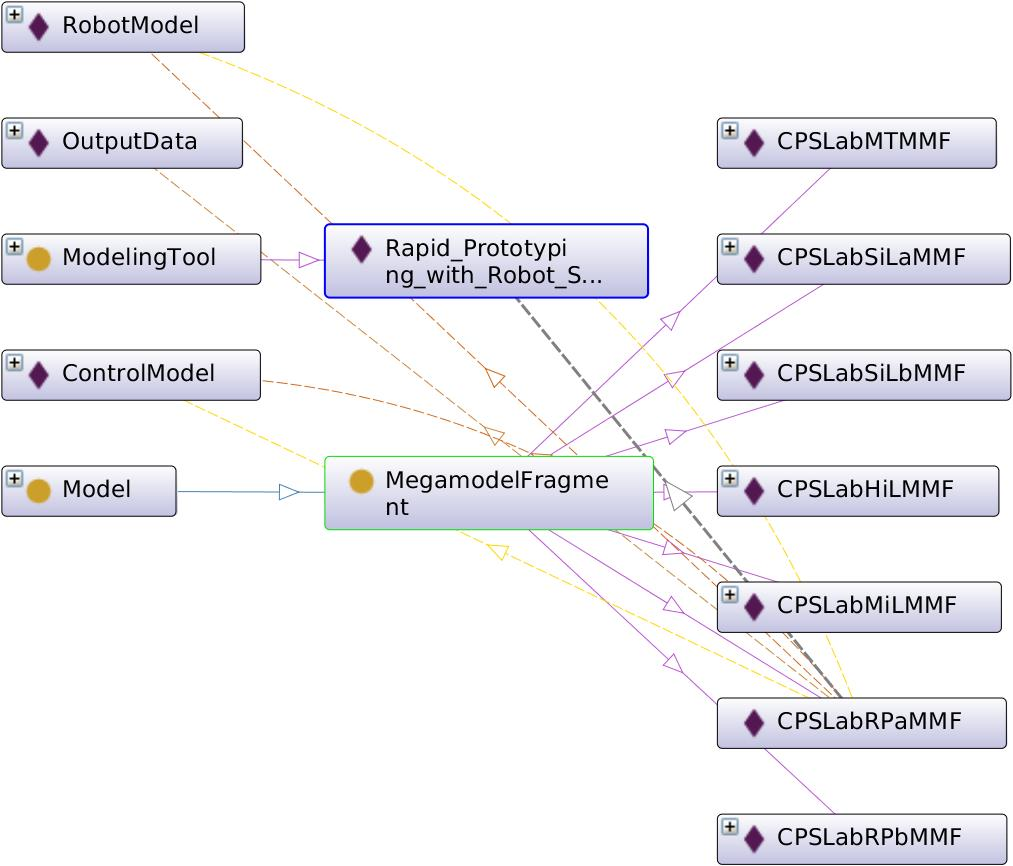
\includegraphics[scale=0.333]{figures/CPSLabRPaMMF.jpg}
\caption{Part of the ontology for the MegaModelFragment \CPSLabRPaMMF covering Rapid Prototyping with Robot Simulation}
\label{fig:CPSLabRPaMMF}
\end{figure}


In Figure~\ref{fig:CPSLabRPaMMF}, the added MegaModel Fragment\uidx{MegamodelFragment} \CPSLabRPaMMF and its elements for the CPSLab ontology outlined in the text are presented.

\LATER{
\subsubsubsubsection{Development Process}
 
FREE TEXT CAPTURING THE ORDERING
}

\subsubsubsubsection{MegaModel Fragment \CPSLabRPbMMF}

\begin{itemize}
    \item MegaModelFragment: \CPSLabRPbMMF
    \begin{itemize}
        \item Model(s): \CPSLabControlModel
    \end{itemize}
\end{itemize}

\subsubsubsubsection{Tools / Models Operations of \CPSLabRPbMMF}

\begin{itemize}
    \item ModelOperation: Rapid Prototyping with Robot Execution
    \begin{itemize}
        \item Input Model(s): \CPSLabControlModel
        \item Output Model(s): Output data (visualized with \MATLABSimulinkSimulator and/or observed)
        \item Employed Tool: \MATLABSimulinkSimulator, \RobotExecutionRemote \COMMENT{\tiny THIS ENTRY IS NOT COVERED BY THE ONTOLOGY SO FAR}
    \end{itemize}
\end{itemize}

\LATER{
\subsubsubsubsection{Development Process}
 
FREE TEXT CAPTURING THE ORDERING
}

\begin{figure}[!htb]
\centering
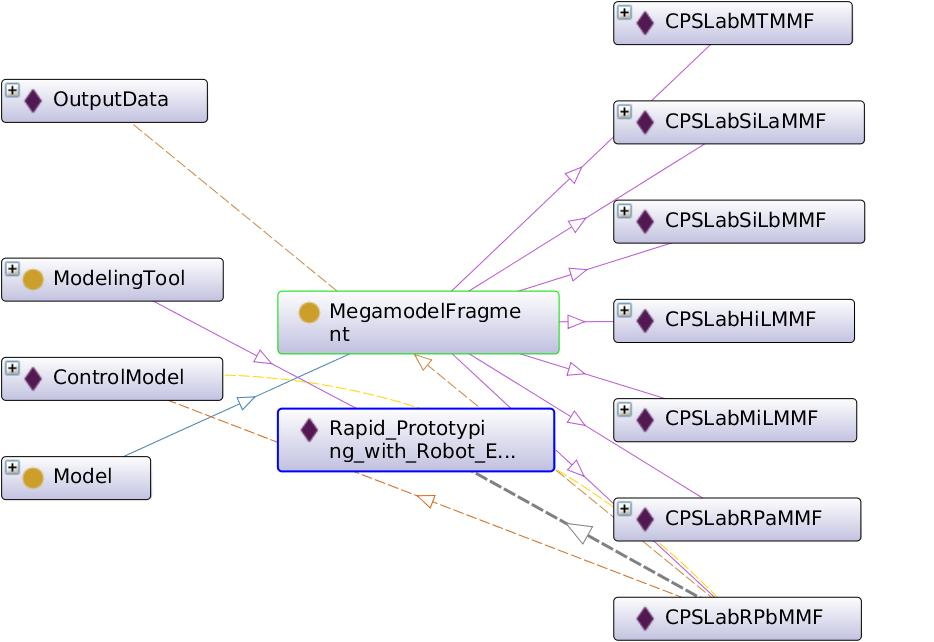
\includegraphics[scale=0.333]{figures/CPSLabRPbMMF.jpg}
\caption{Part of the ontology for MegaModelFragment \CPSLabRPbMMF covering Rapid Prototyping with Robot Execution}
\label{fig:CPSLabRPbMMF}
\end{figure}


The added MegaModel Fragment \CPSLabRPbMMF and its elements for the CPSLab ontology outlined in the text are depicted also in Figure~\ref{fig:CPSLabRPbMMF}.

\DONE[HG]{ HG: please add scheme for MPM ontology use here! }
\DONE[SB]{ HG: please model scheme for MPM ontology presented here with Protege! }
\DONE[SB]{ HG: please add figure showing the used MPM ontology elements here! }



% =========================================
\subsubsubsection{Simulation Stage - MPM Ontology}
%
Some issues are not yet covered by the MPM ontology and the employed megamodel\uidx{Megamodel} and megamodel fragments\uidx{MegamodelFragment}: 
%
While the same types of models and tools are employed at several stages and activities as visible in the megamodel depicted in Figure~\ref{fig:MMFig10}, the models developed for each of these activities are quite different in the simulation stage.
%
For the model test, only simply MATLAB Simulink models with the standard block set and input signals are usually employed. 
%
For the model-in-the-loop simulation, both the model of the control behavior and of the related fragment of the plant are modeled and evaluated using MATLAB/Simulink models with the standard block set.
%
To link the behavior to the FESTO Robotino{\copyright}Sim Simulator and visualize the outcome with FESTO Robotino{\copyright}View, a specific block set compatible with the FESTO Robotino-Library is employed.






% ===============================================
\subsubsection{Prototyping}
%


% ============================================
\subsubsection{Software in the Loop (SiL)}
%
Software in the Loop (SiL) as introduced in Figure~\ref{fig:sil}, can actually be done in different ways:
%
A first version executes the generated software on a desktop computer and runs it against a simulator as depicted in Figure~\ref{fig:MMFig7}.

\begin{figure}[!htb]
\centering
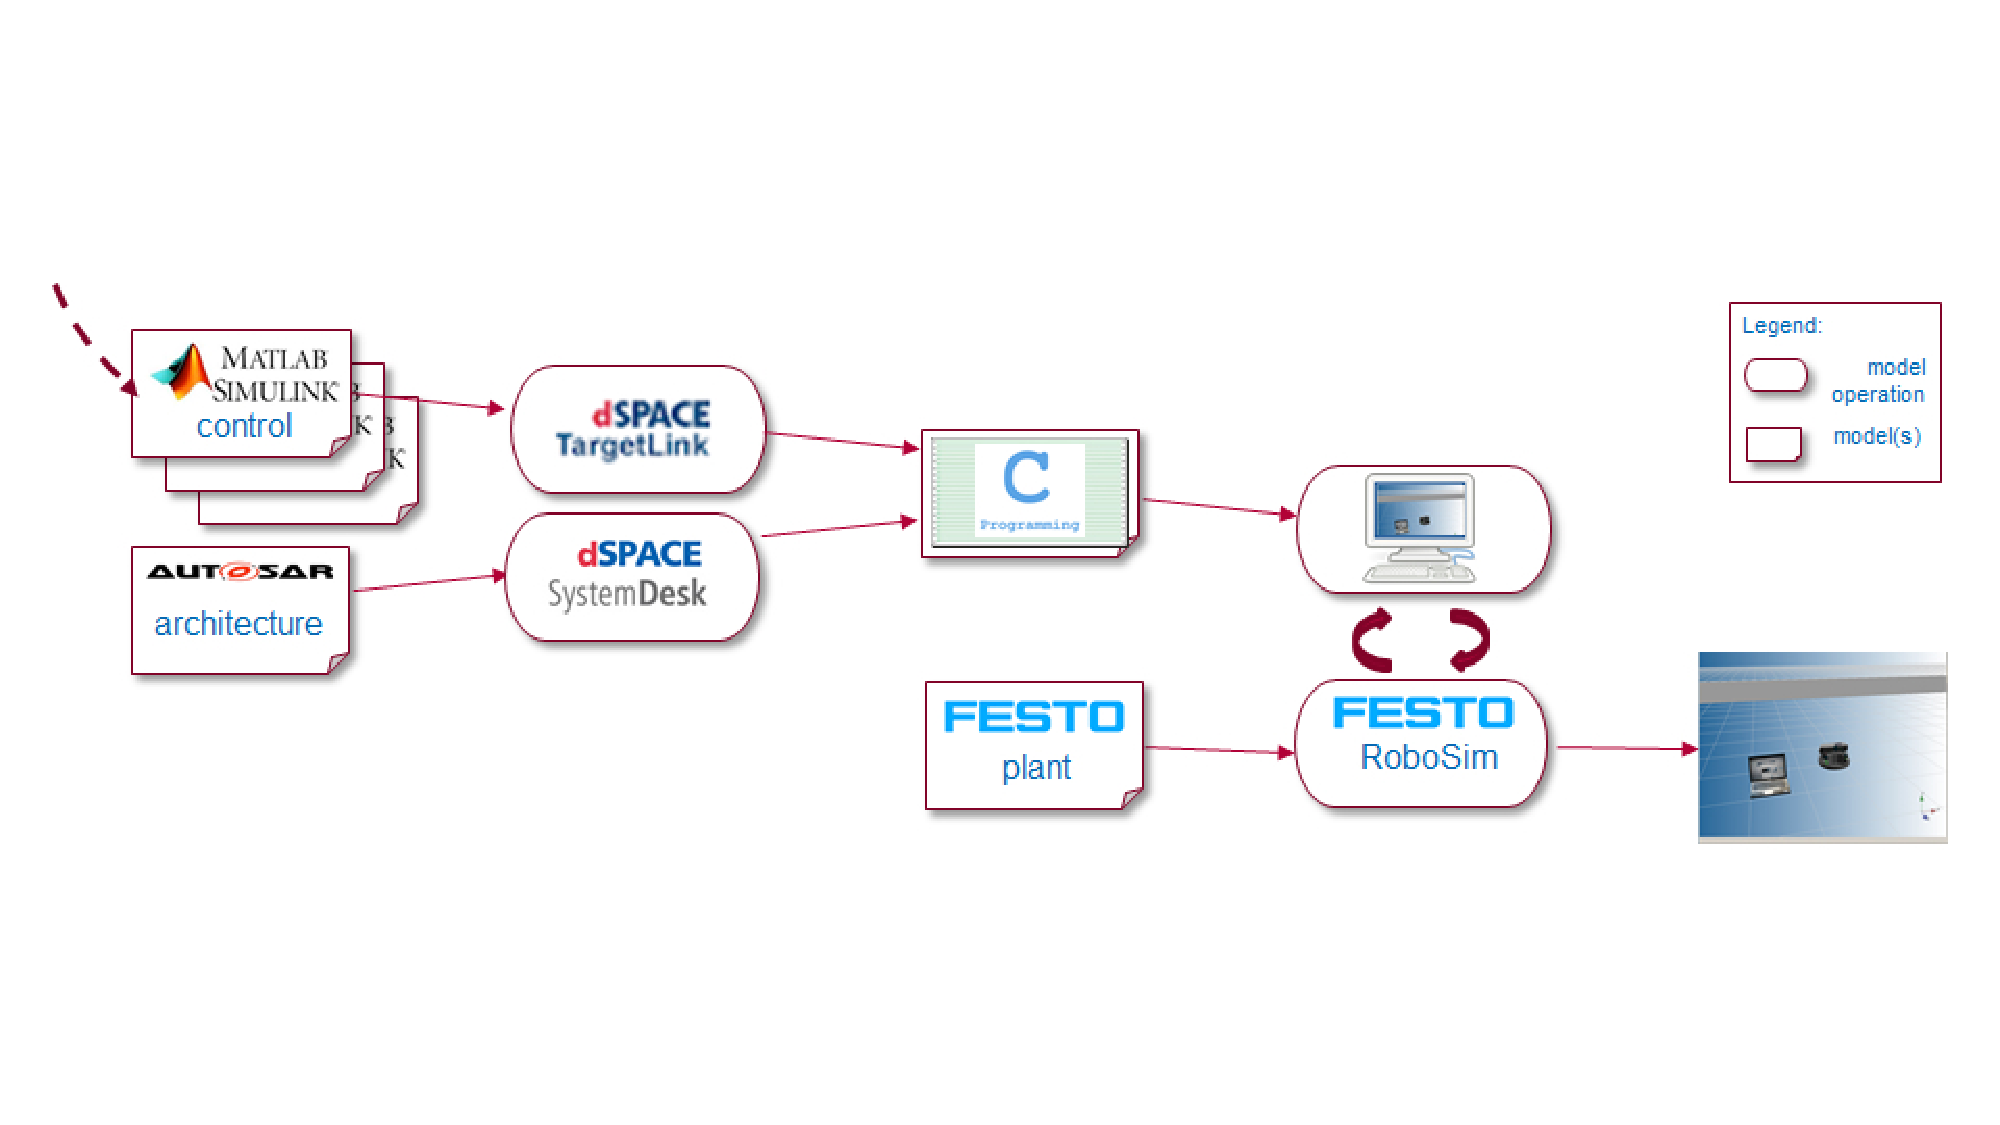
\includegraphics[scale=0.33]{figures/mm-hpi7.pdf}
\caption{Software in the Loop (SiL) vs. Desktop + Sim}
\label{fig:MMFig7}
\end{figure}

A second form executes the generated software  on a desktop computer and in contrast to the first form links it to the robot as depicted in Figure~\ref{fig:MMFig8}.

\begin{figure}[!htb]
\centering
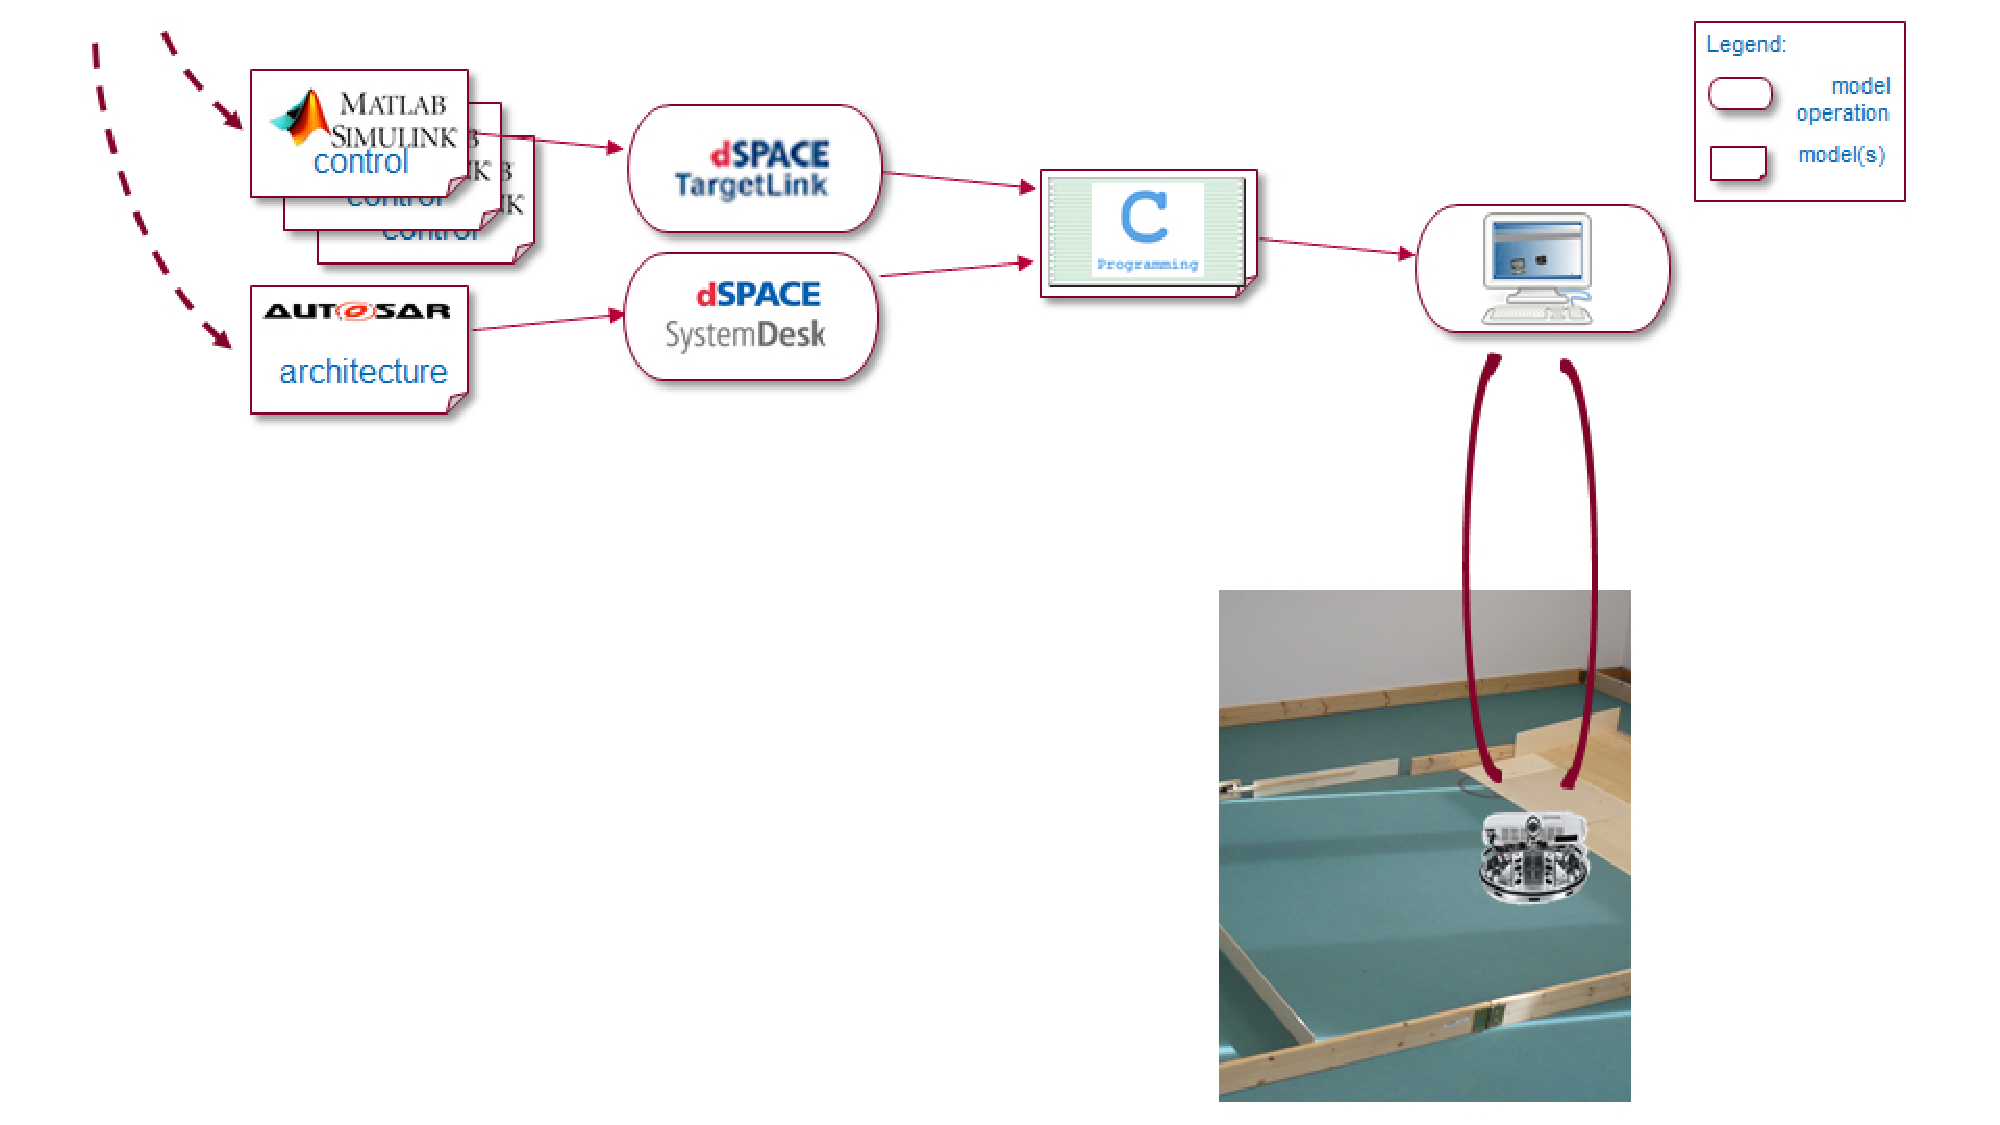
\includegraphics[scale=0.33]{figures/mm-hpi8.pdf}
\caption{Software in the Loop (SiL) vs. Desktop + Robot}
\label{fig:MMFig8}
\end{figure}

% =========================================
\subsubsubsection{Software in the Loop (SiL) - MPM Ontology}
%
\subsubsubsubsection{MegaModel Fragment \CPSLabSiLaMMF}

\begin{itemize}
    \item MegaModelFragment: \CPSLabSiLaMMF
    \begin{itemize}
        \item Model(s): \CPSLabControlModel*, \CPSLabSystemModel, \CPSLabRobotModel
    \end{itemize}
\end{itemize}

\subsubsubsubsection{Tools / Models Operations of \CPSLabSiLaMMF}

\begin{itemize}
    \item ModelOperation: FunctionCodeGeneration*
    \begin{itemize}
        \item Input Model(s): \CPSLabControlModel
        \item Output Model(s): \CPSLabControlModelCode
        \item Employed Tool: \dSPACETargetLink \COMMENT{\tiny THIS ENTRY IS NOT COVERED BY THE ONTOLOGY SO FAR}
    \end{itemize}
    \item ModelOperation: SystemCodeGeneration
    \begin{itemize}
        \item Input Model(s): \CPSLabSystemModel
        \item Output Model(s): \CPSLabSystemModelCode
        \item Employed Tool: \dSPACESystemDesk \COMMENT{\tiny THIS ENTRY IS NOT COVERED BY THE ONTOLOGY SO FAR}
    \end{itemize}
    \item ModelOperation: Software-in-the-Loop Simulation
    \begin{itemize}
        \item Input Model(s): \CPSLabControlModelCode*, \CPSLabSystemModelCode, \CPSLabRobotModel
        \item Output Model(s): Output data (visualized with \MATLABSimulinkSimulator and/or \FESTORobotinoView)
        \item Employed Tool: \DesktopExecution, \FESTORobotinoSim \COMMENT{\tiny THIS ENTRY IS NOT COVERED BY THE ONTOLOGY SO FAR}
    \end{itemize}
\end{itemize}

\LATER{
\subsubsubsubsection{Development Process}
 
FREE TEXT CAPTURING THE ORDERING
}

\begin{figure}[!htb]
\centering
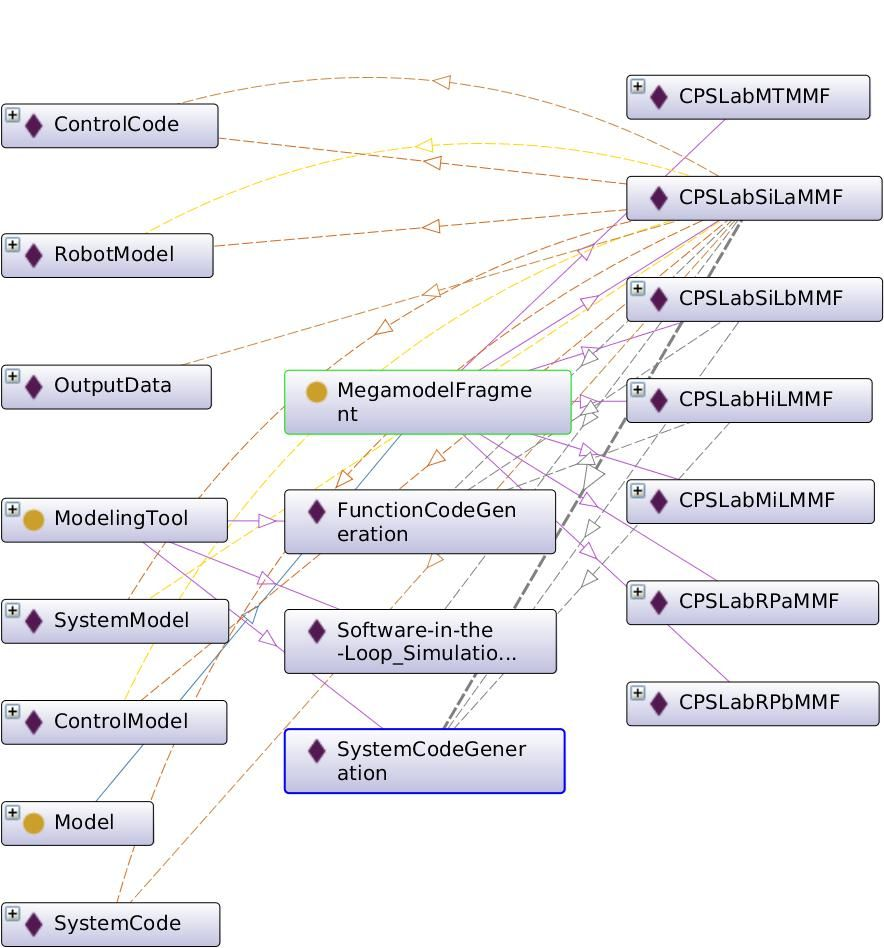
\includegraphics[scale=0.333]{figures/CPSLabSiLaMMF.jpg}
\caption{Part of the ontology for the MegaModelFragment \CPSLabSiLaMMF covering SiL with Simulation}
\label{fig:CPSLabSiLaMMF}
\end{figure}

The added MegaModel Fragment \CPSLabSiLaMMF and its elements for the CPSLab ontology outlined in the text are depicted also in Figure~\ref{fig:CPSLabSiLaMMF}.


\DONE[HG]{ HG: please add scheme for MPM ontology use here! }
\DONE[SB]{ HG: please model scheme for MPM ontology presented here with Protege! }
\DONE[SB]{ HG: please add figure showing the used MPM ontology elements here! }

\subsubsubsubsection{MegaModel Fragment \CPSLabSiLbMMF}

\begin{itemize}
    \item MegaModelFragment: \CPSLabSiLbMMF
    \begin{itemize}
        \item Model(s): \CPSLabControlModel*, \CPSLabSystemModel
    \end{itemize}
\end{itemize}

\subsubsubsubsection{Tools / Models Operations of \CPSLabSiLbMMF}

\begin{itemize}
    \item ModelOperation: FunctionCodeGeneration*
    \begin{itemize}
        \item Input Model(s): \CPSLabControlModel
        \item Output Model(s): \CPSLabControlModelCode
        \item Employed Tool: \dSPACETargetLink \COMMENT{\tiny THIS ENTRY IS NOT COVERED BY THE ONTOLOGY SO FAR}
    \end{itemize}
    \item ModelOperation: SystemCodeGeneration
    \begin{itemize}
        \item Input Model(s): \CPSLabSystemModel
        \item Output Model(s): \CPSLabSystemModelCode
        \item Employed Tool: \dSPACESystemDesk \COMMENT{\tiny THIS ENTRY IS NOT COVERED BY THE ONTOLOGY SO FAR}
    \end{itemize}
    \item ModelOperation: Software-in-the-Loop Execution
    \begin{itemize}
        \item Input Model(s): \CPSLabControlModelCode*, \CPSLabSystemModelCode
        \item Output Model(s): Output data (visualized with \MATLABSimulinkSimulator and/or observed)
        \item Employed Tool: \RobotExecutionRemote, \DesktopExecution \COMMENT{\tiny THIS ENTRY IS NOT COVERED BY THE ONTOLOGY SO FAR}
    \end{itemize}
\end{itemize}

\LATER{
\subsubsubsubsection{Development Process}
 
FREE TEXT CAPTURING THE ORDERING
}

\DONE[HG]{ HG: please add scheme for MPM ontology use here! }
\DONE[SB]{ HG: please model scheme for MPM ontology presented here with Protege! }
\DONE[SB]{ HG: please add figure showing the used MPM ontology elements here! }

\begin{figure}[!htb]
\centering
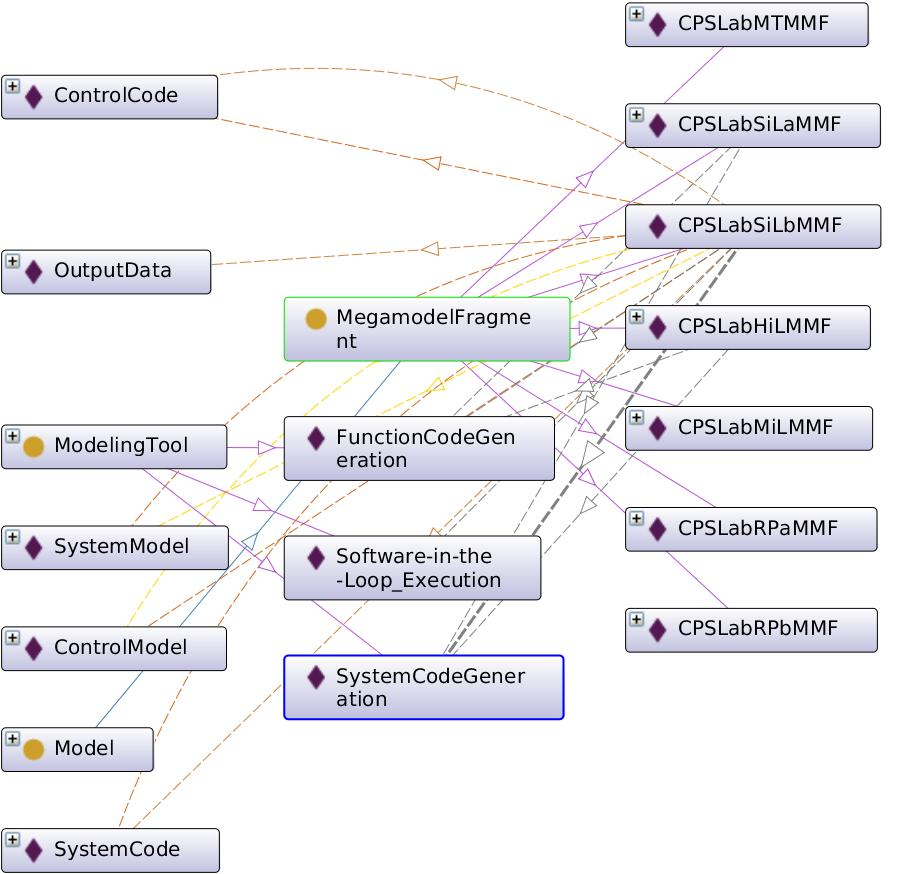
\includegraphics[scale=0.333]{figures/CPSLabSiLbMMF.jpg}
\caption{Part of the ontology for the MegaModelFragment\uidx{MegamodelFragment} \CPSLabSiLbMMF covering Sil with Execution}
\label{fig:CPSLabSiLbMMF}
\end{figure}

The added MegaModel Fragment \CPSLabSiLbMMF and its elements for the CPSLab ontology outlined in the text are depicted also in Figure~\ref{fig:CPSLabSiLbMMF}.


% ============================================
\subsubsection{Hardware in the Loop (HiL)}
%
Hardware in the Loop (HiL) as introducted in Figure~\ref{fig:hil} in contrast links the generated software such that it can be executed on the robot as depicted in Figure~\ref{fig:MMFig9}.

\begin{figure}[!htb]
\centering
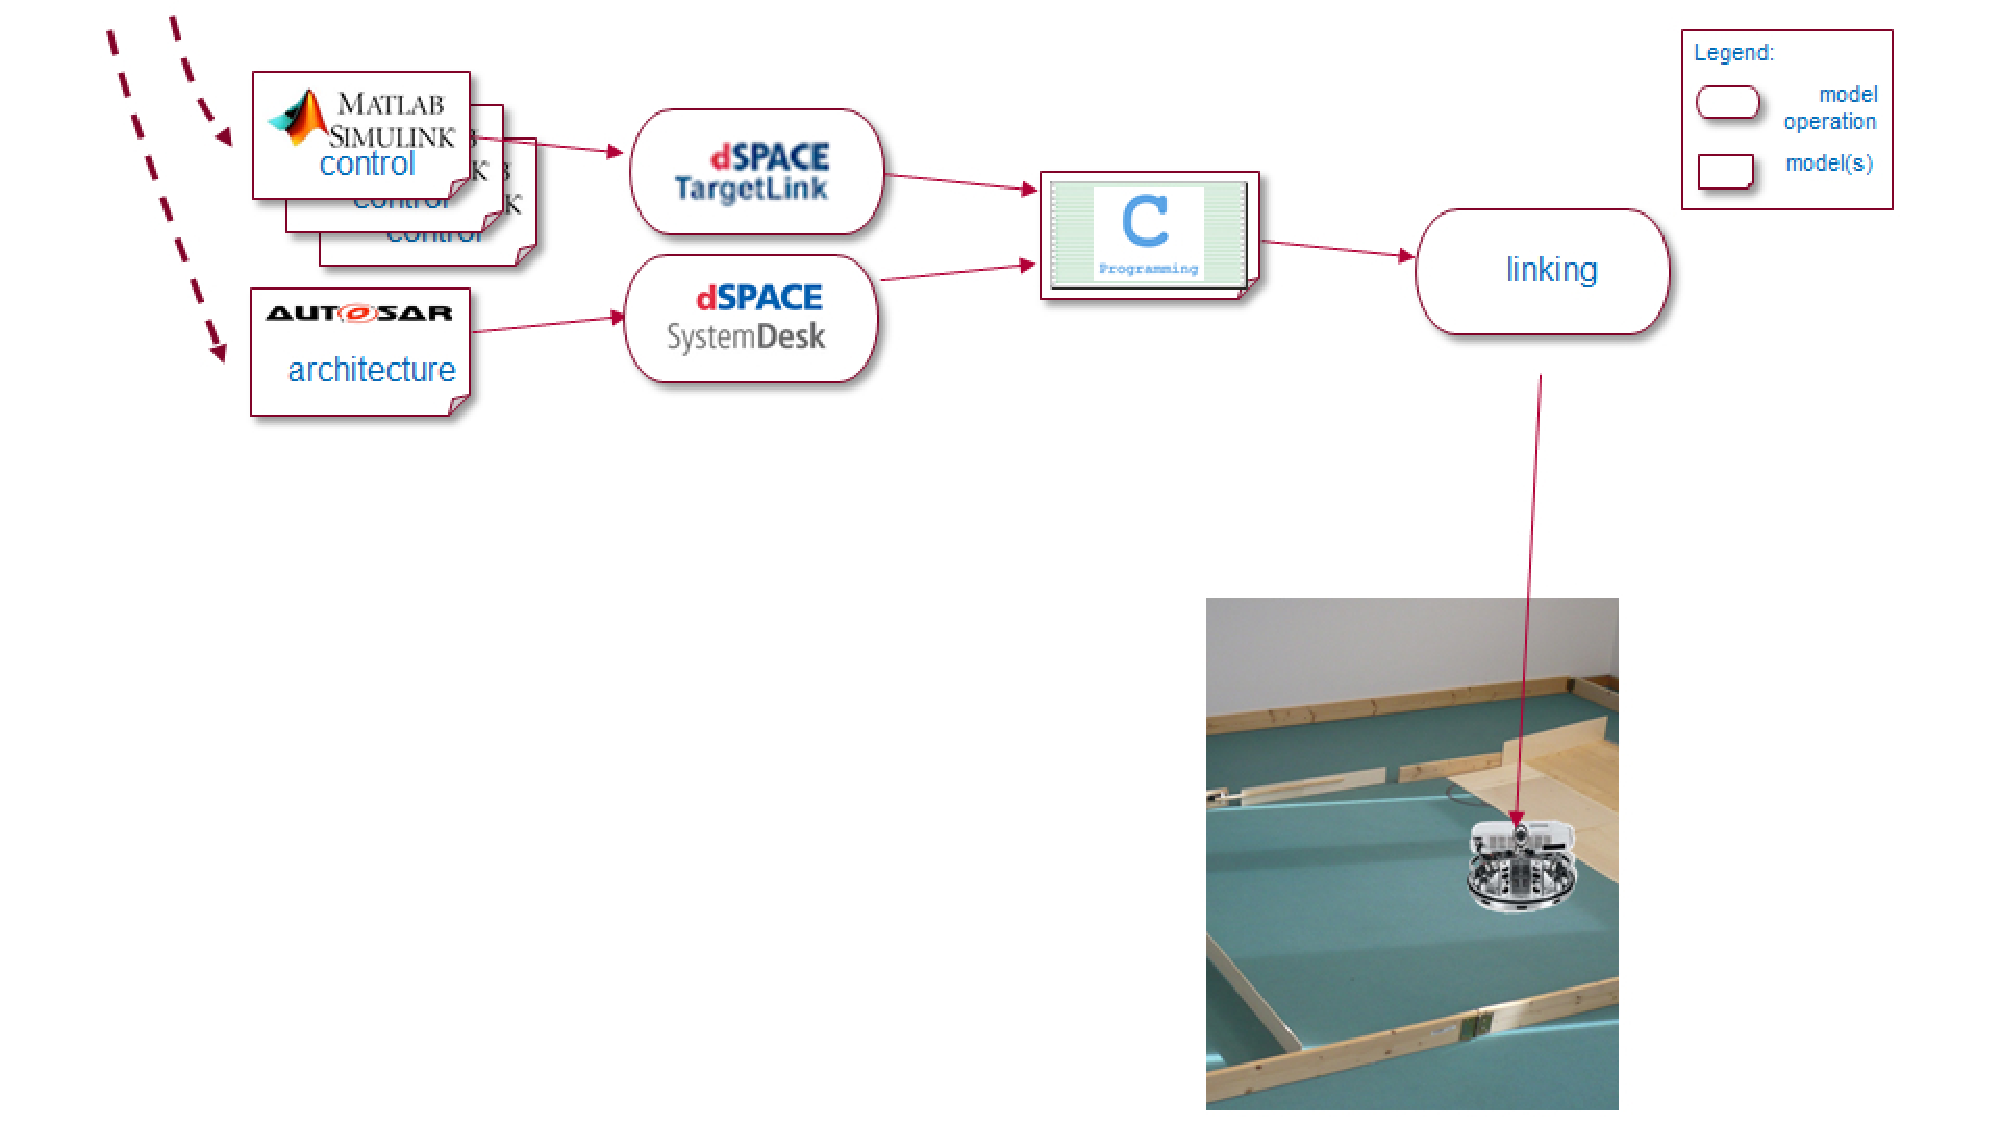
\includegraphics[scale=0.33]{figures/mm-hpi9.pdf}
\caption{Hardware in the Loop (HiL)}
\label{fig:MMFig9}
\end{figure}

% =========================================
\subsubsubsection{Hardware in the Loop (HiL) - MPM Ontology}
%
\subsubsubsubsection{MegaModel Fragment \CPSLabHiLMMF}

\begin{itemize}
    \item MegaModelFragment: \CPSLabHiLMMF
    \begin{itemize}
        \item Model(s): \CPSLabControlModel*, \CPSLabSystemModel
    \end{itemize}
\end{itemize}

\subsubsubsubsection{Tools / Models Operations of \CPSLabHiLMMF}

\begin{itemize}
    \item ModelOperation: FunctionCodeGeneration*
    \begin{itemize}
        \item Input Model(s): \CPSLabControlModel
        \item Output Model(s): \CPSLabControlModelCode
        \item Employed Tool: \dSPACETargetLink \COMMENT{\tiny THIS ENTRY IS NOT COVERED BY THE ONTOLOGY SO FAR}
    \end{itemize}
    \item ModelOperation: SystemCodeGeneration
    \begin{itemize}
        \item Input Model(s): \CPSLabSystemModel
        \item Output Model(s): \CPSLabSystemModelCode
        \item Employed Tool: \dSPACESystemDesk \COMMENT{\tiny THIS ENTRY IS NOT COVERED BY THE ONTOLOGY SO FAR}
    \end{itemize}
    \item ModelOperation: Hardware-in-the-Loop Execution
    \begin{itemize}
        \item Input Model(s): \CPSLabControlModelCode*, \CPSLabSystemModelCode
        \item Output Model(s): Output data (observed)
        \item Employed Tool: \RobotExecutionLocal \COMMENT{\tiny THIS ENTRY IS NOT COVERED BY THE ONTOLOGY SO FAR}
    \end{itemize}
\end{itemize}

\LATER{
\subsubsubsubsection{Development Process}
 
FREE TEXT CAPTURING THE ORDERING
}

\DONE[HG]{ HG: please add scheme for MPM ontology use here! }
\DONE[SB]{ HG: please model scheme for MPM ontology presented here with Protege! }
\DONE[SB]{ HG: please add figure showing the used MPM ontology elements here! }

\begin{figure}[!htb]
\centering
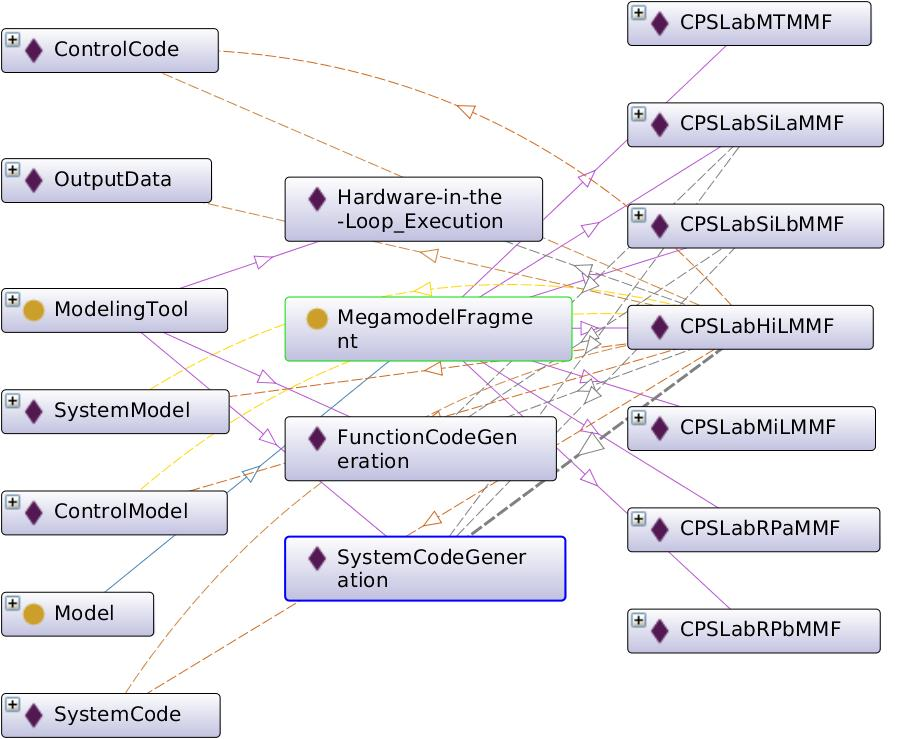
\includegraphics[scale=0.333]{figures/CPSLabHiLMMF.jpg}
\caption{Part of the ontology for the MegaModelFragment \CPSLabHiLMMF covering Hil}
\label{fig:MMF-HPI-HiL}
\end{figure}

The added MegaModel Fragment\uidx{MegamodelFragment} \CPSLabHiLMMF and its elements for the CPSLab ontology outlined in the text are depicted also in Figure~\ref{fig:MMF-HPI-HiL}.


% =========================================
\subsubsubsection{Prototyping - MPM Ontology}
%
Again, the MPM ontology and the employed megamodel\uidx{Megamodel} and megamodel fragments\uidx{MegamodelFragment} do not cover all issues: 
%
In contrast to the restriction to MATLAB/Simulink during the simulation stage, for the prototyping stage also dSPACE SystemDesk for describing a component-based\uidx{Component} architecture with AUTOSAR must be considered as well as outlined above and depicted in the megamodel presented in Figure~\ref{fig:MMFig10}.
%
For the software-in-the-loop simulation, it is necessary to adjust the functional models to the specific dSPACE TargetLink block set such that the dSPACE TargetLink for code generation can be employed. In addition, dSPACE SystemDesk is employed to define the software architecture, hardware configuration, and task mapping with AUTOSAR. Then, this combination of models is linked via the blocks for the FESTO Robotino-Library and simulated by linking the MATLAB/Simulink and FESTO Robotino{\copyright}Sim simulators and  the outcome is visualized with FESTO Robotino{\copyright}View. 
%
In case of the hardware-in-the-loop testing, the same block set for the FESTO Robotino-Library can be reconfigured such that 
%
either the compiled software runs on a host computer and controls the Robotino robots remotely
%
or the compiled and linked software runs directly on the Robotino robots.


\LATER[one advanced scenario]{
% ============================================
\subsubsection{Advanced Scenario}\label{subsubsec:cpslab-mpm-advanced}
\marginpar{WORK EXAMPLE: hopefully complex enough to require most elements of the ontology}%
%
A more complex scenario featuring the horizontal combination of multiple specific structures in form of AUTOSAR for the software, VHDL for the hardware, and Matlab/Modelica for the plant linked together via a generic system structure in form of a SysML model is depicted in Figure~\ref{fig:MMFig16}.
%
\TODOINLINE{ HG: add refs for work that has been done and explain what is hypothetical }

\begin{figure}[!htb]
\centering
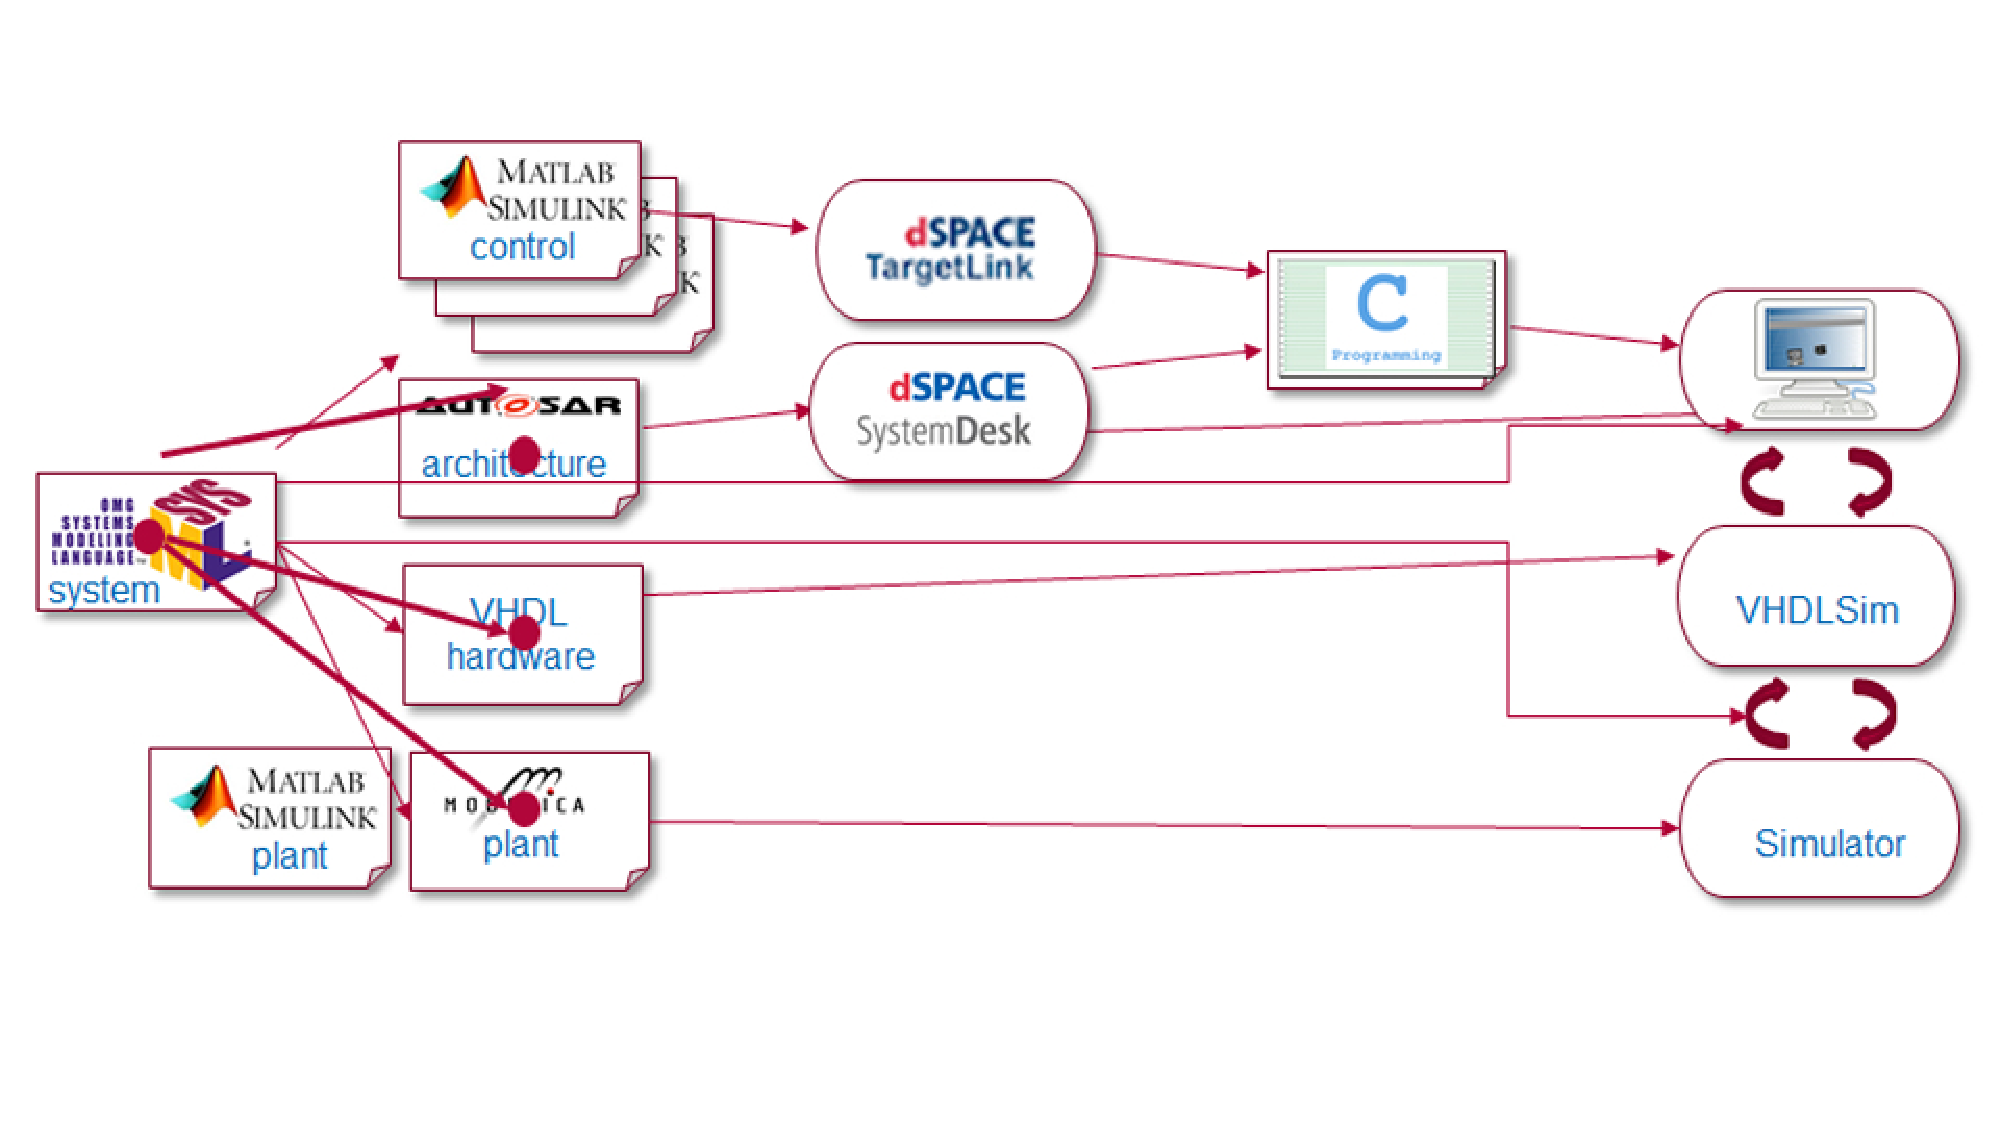
\includegraphics[scale=0.33]{figures/mm-hpi16.pdf}
\caption{Scenario: More Complex Horizontal Integration}
\label{fig:MMFig16}
\end{figure}

\marginpar{WORK EXAMPLE: try to capture what is in Figure~\ref{fig:MMFig16} with the ontology}
%

CPSLabMM : MegaModel (): for CPSLab

- hasMegaModelFragment (3.4.10): CPSLabMM <-> CPSLabMM::Advanced

CPSLabMM::Advanced : MegaModelFragment (3.3.3.6): whole Figure~\ref{fig:MMFig16}

TargetLinkMO : ModelOperation (3.3.3.10): code generation using TargetLink

- hasInput (3.4.7): multiple Matlab/Simulink control models for different functions

. hasOutput (3.4.16): multipl C-code models for each function covered by one control model

SystemDeskMO : ModelOperation (3.3.3.10): code generation for the architecture using SystemDesk

- hasInput (3.4.7): one AUTOSAR architecture model referencing the different functions

. hasOutput (3.4.16):  C-code models for the architecture integrating all function covered by the control model

CoSimulationMO : ModelOperation (3.3.3.10): co-executes and co-simulates the AUTOSAR, VHDL, and plant model

- hasInput (3.4.7): 

-- one SysML architecture model referencing the different architectures

-- one AUTOSAR architecture model referencing the different functions

-- one VVHDL  model 

-- one Modelica/Matlab plant model 

. hasOutput (3.4.16):  simuzlation outcome

OPEN QUESTION: How is this complex model operation linked to the involved tools? Do we use multiple model operations and lomnk them or does the mode operation reference simply multiple tools?

REMARK: possibly required additional tools that allow to link the simulators are missing ...

\subsection*{MegamModel Fragments}
\begin{itemize}
    \item robotControl Validation
\end{itemize}

% ============================================
%\subsubsection{MPM Ontology}\label{subsubsec:cpslab-mpm-needs}
%
\TODOINLINE{ HG: add needs for the MPM ontology and catalog that are present in the case study? 

- define all required ModelOperations with its hasInput and hasOutput

- link ModelOperations to the Tools (in case of co-simulation one model operation links multiple tools!)



- constrain Models with the specific needs as outlined in the text (e.g., use of block sets etc.)



}
}

% ========================================================================================
\subsection{MPM4CPS}\label{subsec:cpslab-mpm4cps}
%
In order to discuss the role of MPM for CPS development as presented in the case study, we refer to the inherent integration needs underlying the development of embedded real-time systems and cyber-physical systems in particular as outlined in \cite{GieseNNS2011}. Furthermore, we link these observations to the MPM4CPS ontology as presented in Chapter~\ref{ch:mpm4cps} and further needs to extend it.

% ============================================
\subsubsection{Simulation Stage}
%
% =========================================
\subsubsubsection{Model Test}
%
In the model test as outlined in Figure~\ref{fig:MMFig3} and in its megamodel fragment\uidx{MegamodelFragment}, the abstract control algorithm from the cyber domain captured by the Matlab/Simulink model (\CPSLabControlModel) for the control is confronted with the physics as present in the input data plus expected outcomes and thus we have a very simple cyber-physical setting. We further often have a multi-formalism setting as the control is discrete\uidx{DiscreteCharacteristic} while the input is at least conceptually continuous\uidx{ContinuousCharacteristic}. 

\TODONOTE{ HG: viewpoint: plausible control behavior, concern: robust control }

% =========================================
\subsubsubsection{Model-in-the-Loop}
%
The model in the loop depicted in Figure~\ref{fig:MMFig4} and in its megamodel fragment\uidx{MegamodelFragment} in contrast, the abstract control algorithm from the cyber domain captured by the Matlab/Simulink model (\CPSLabControlModel) is combined with the idealized physics as present in the plant captured by the Matlab/Simulink model (\CPSLabPlantModel) and thus we have a simple cyber-physical setting. We again often have a multi-formalism setting as the control is discrete\uidx{DiscreteCharacteristic} while the input is at least conceptually continuous\uidx{ContinuousCharacteristic}. 

\TODONOTE{ HG: viewpoint: suitable control behavior, concern: robust control }


% =========================================
\subsubsubsection{Rapid Prototyping}
%
Our rapid prototyping based on a sophisticated robot simulator as depicted in Figure~\ref{fig:MMFig5} and in its megamodel fragment\uidx{MegamodelFragment}, again the abstract control algorithm from the cyber domain captured by the Matlab/Simulink model (\CPSLabControlModel) is brought together with the physics as present in the sophisticated robot model (\CPSLabRobotModel) of the simulator and thus we have clearly a cyber-physical setting. We again often have a multi-formalism setting as the control is discrete\uidx{DiscreteCharacteristic}, while the sophisticated model of the robot simulation is at least conceptually continuous\uidx{ContinuousCharacteristic}. Consistency is checked via co-simulation as the simulator for the robot model runs in parallel with the sophisticated robot simulator.\todo{What is the other simulator?}

The rapid prototyping against the robot as depicted in Figure~\ref{fig:MMFig6} and in its megamodel fragment\uidx{MegamodelFragment}, the abstract control algorithm from the cyber domain captured by the Matlab/Simulink model (\CPSLabControlModel) is brought together with the real physics of the robot  and thus we have clearly a cyber-physical setting. Consistency is checked via co-simulation as the simulator for the robot model runs in parallel with the robot.

\TODONOTE{ HG: viewpoint: really suitable control behavior, concern: robust control }


% ============================================
\subsubsection{Prototyping}
%

% ============================================
\subsubsection{Software in the Loop (SiL)}
%
The first form of software in the loop (SiL) executing the software on a desktop computer against a simulator as depicted in Figure~\ref{fig:MMFig7} and in its megamodel fragment features that the detailed control algorithm from the cyber domain captured by the Matlab/Simulink and AUTOSAR SystemDesk models (\CPSLabSystemModels) are brought together with the physics as present in the sophisticated robot model of the simulator (\CPSLabRobotModel) and thus we have clearly a cyber-physical setting. We again often have a multi-formalism setting as the control is discrete\uidx{DiscreteCharacteristic} while the sophisticated robot mode is at least conceptually continuous\uidx{ContinuousCharacteristic}. Consistency is checked via co-simulation as the software for the robot control runs in parallel with the sophisticated robot simulator.


The second form of software in the loop (SiL) executing the software on a desktop computer against a remote controlled robot depicted in Figure~\ref{fig:MMFig8} and in its megamodel fragment ensures that the detailed control algorithm from the cyber domain captured by the Matlab/Simulink model and AUTOSAR SystemDesk models (\CPSLabSystemModels) are brought together with the physics as present in the remote controlled robot and thus we have clearly a cyber-physical setting. Consistency is checked via co-execution as the software for the robot control runs in parallel with the remote controller robot.

\TODONOTE{ HG: viewpoint: suitable system behavior, concern: robust overall control }

% ============================================
\subsubsection{Hardware in the Loop (HiL)}
%
The hardware in the loop (HiL) executing the software on the robot depicted in Figure~\ref{fig:MMFig8} and in its megamodel fragment ensures that the detailed control algorithm from the cyber domain aptured by the Matlab/Simulink model (\CPSLabControlModel) is brought together with the physics as present in the robot and thus we have clearly a cyber-physical setting. Consistency is checked via executing the software on the robot.

\TODONOTE{ HG: viewpoint: suitable system behavior, concern: robust overall control }

\TODONOTE{ HG: we have similar concerns that are repeatedly checked with different degrees of detail. Do we need different viewpoint names? }

\LATER[advanced scenarios]{

% ============================================
\subsubsection{Advanced Scenarios}
%

\begin{enumerate}
    \item Vertical enrichment of functional models (consistency manually)
\item Horizontal integration of functional and plant models
\item Horizontal integration of multiple functional models, an architecture model, and a plant model
\item Vertical enrichment of multiple functional models, an architecture model, and a plant model (to realize functions while meeting resource constraints)
\end{enumerate}

{\bf The Challenge of Model-Based Integration for Cyber-Physical Systems}
\begin{enumerate}
    \item Vertical refinement of functional models (consistency manually)
\item Horizontal integration of functional and plant models
\item Horizontal integration of multiple functional models, an architecture model, and a plant model
\item Vertical refinement of functional models (to realize functions while meeting resource constraints)
\end{enumerate}

KKKKKKKKKKKKK


\begin{figure}[!htb]
\centering
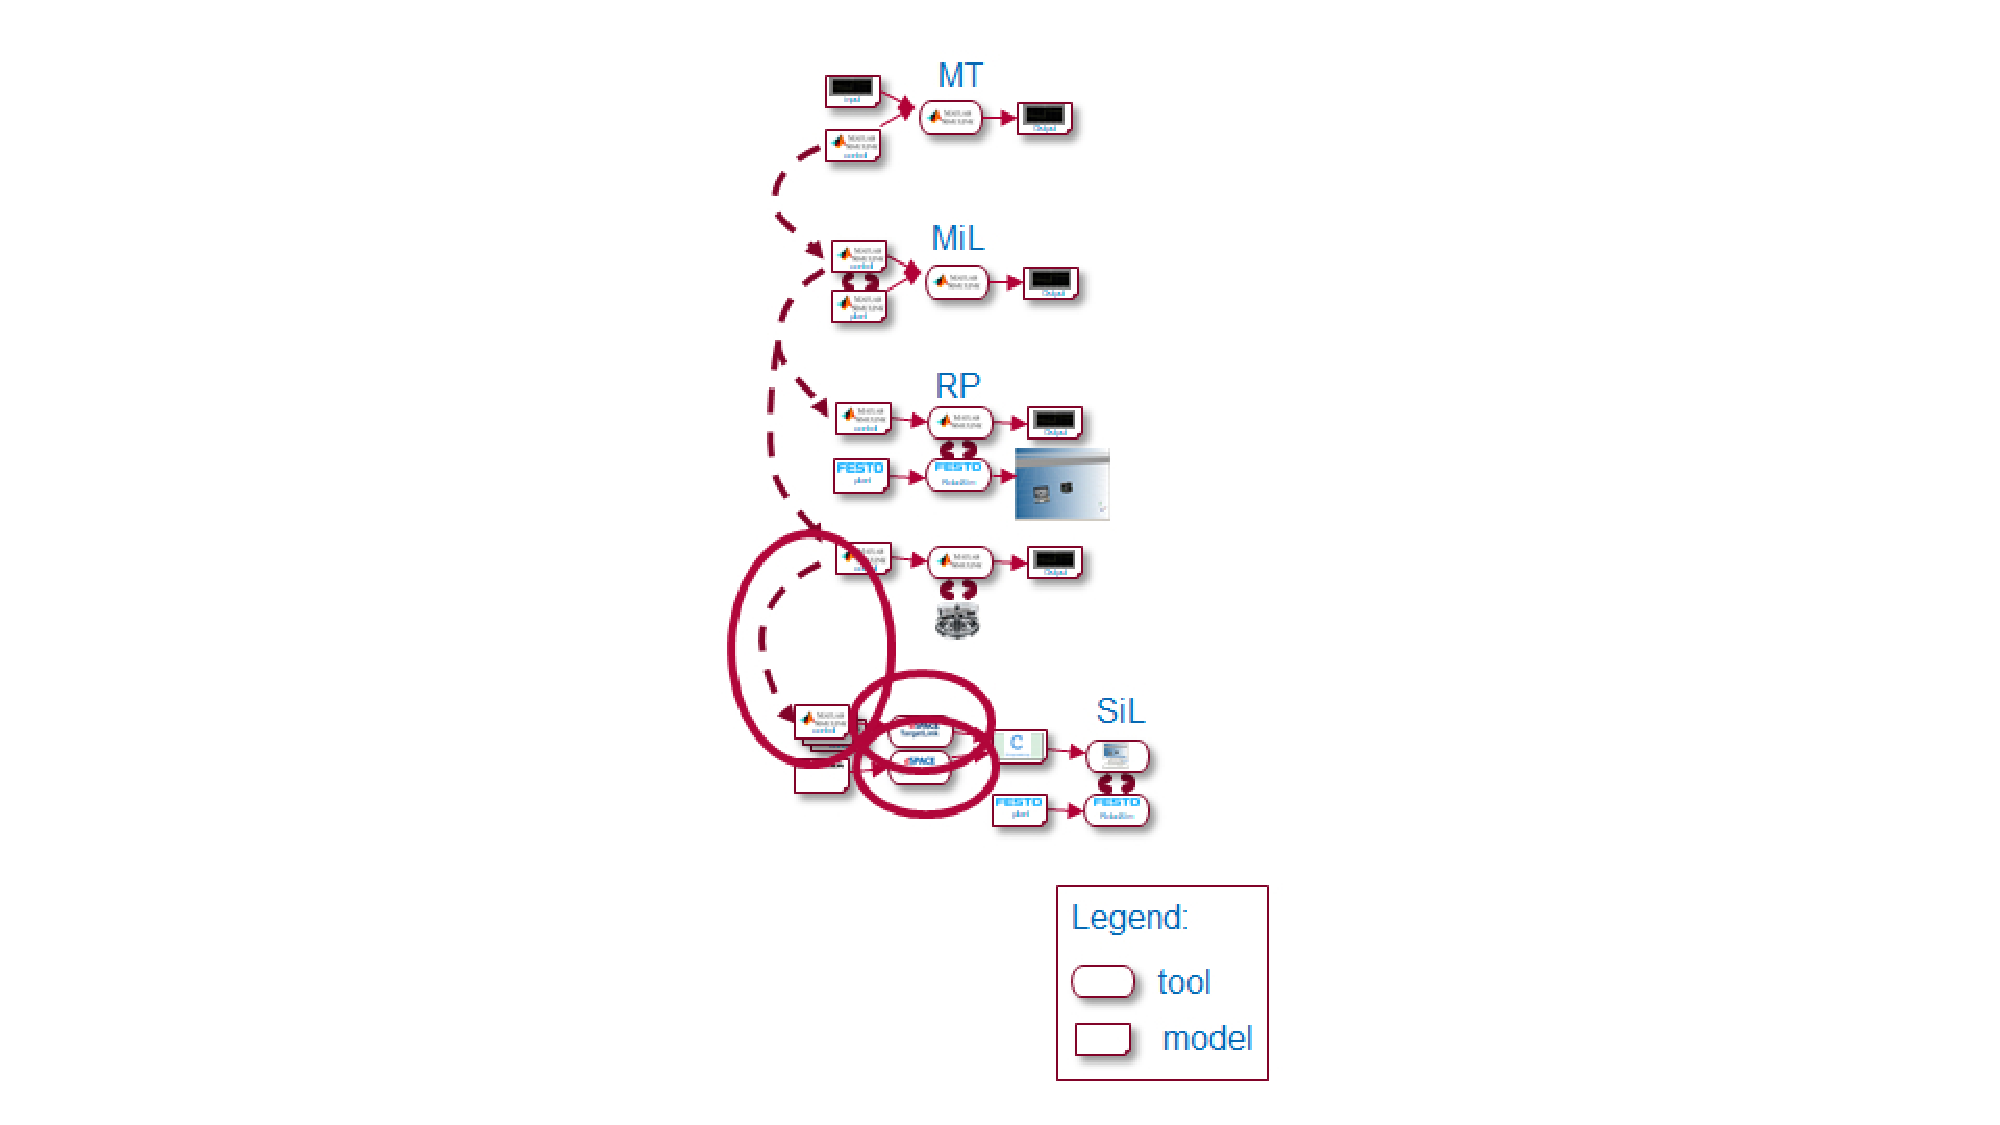
\includegraphics[scale=0.33]{figures/mm-hpi12.pdf}
\caption{Vertical Enrichment and  Transformation}
\label{fig:MMFig11}
\end{figure}

{\bf Vertical Enrichment and  Transformation} Figure~\ref{fig:MMFig11}
\begin{enumerate}
    \item Vertical enrichment of functional models and architecture
\item Floating-Point 2 Fix-Point to reduce resource demands models (consistency manually)
\item Fix-Point data-flow model 2 C-code models (consistency automatically)
\item Autosar 2 C-code models (consistency automatically)
\end{enumerate}

\begin{figure}[!htb]
\centering
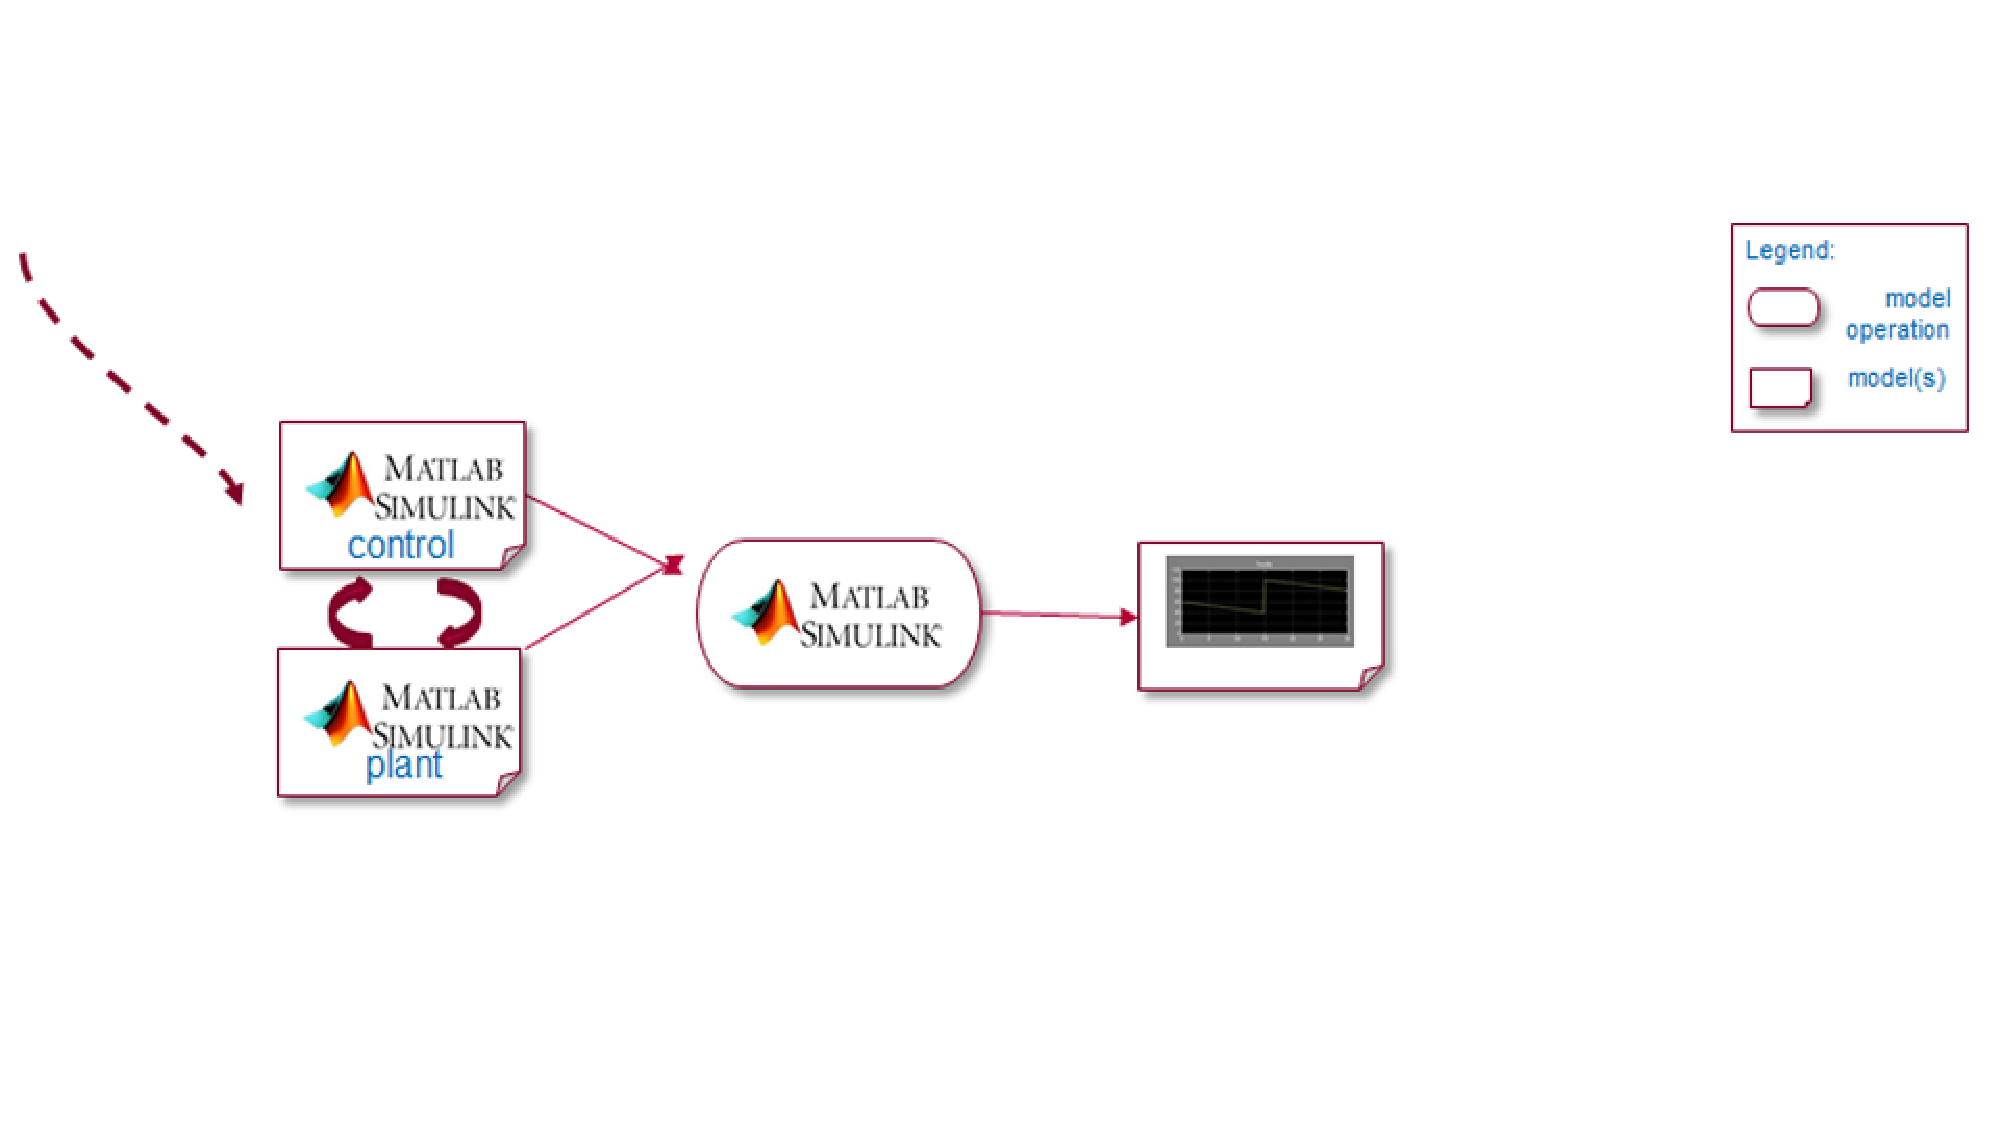
\includegraphics[scale=0.33]{figures/mm-hpi14.pdf}
\caption{Model in the Loop (MiL)}
\label{fig:MMFig12}
\end{figure}

{\bf Model in the Loop (MiL)} Figure~\ref{fig:MMFig12}

\begin{enumerate}
    \item Layer: Abstract Control Algorithm + Idealized Plant
\item Domain: Control/Software + Physics
\item Multi-Paradigm: Yes, if control is discrete 
\item Cyber-Physical system: Yes, as control is cyber world and plant is from the physical world
\item Integration: Decomposition and Composition + parallel development; semantics-level
\end{enumerate}

\begin{figure}[!htb]
\centering
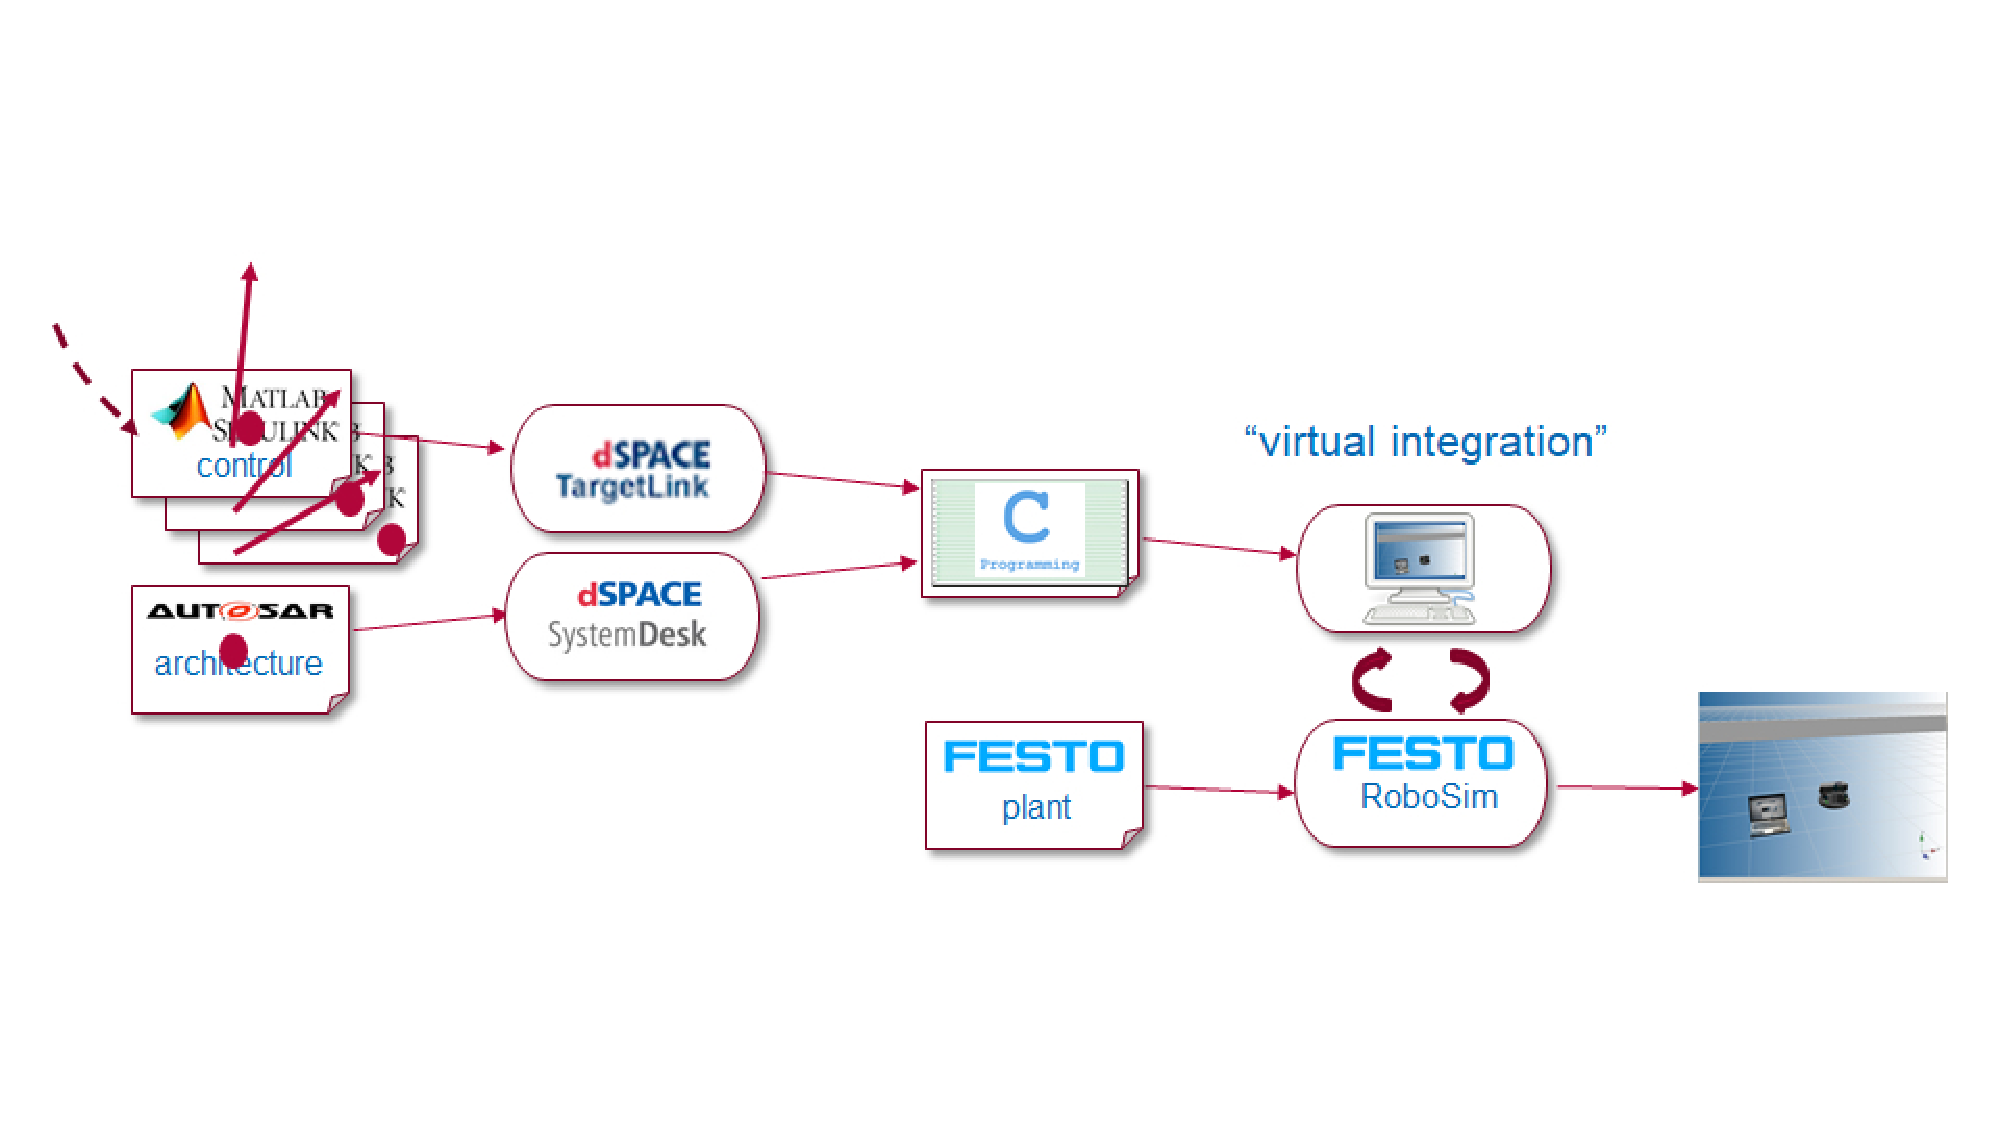
\includegraphics[scale=0.33]{figures/mm-hpi15.pdf}
\caption{Scenario: Complex Horizontal Integration}
\label{fig:MMFig13}
\end{figure}
\newpage
{\bf Scenario: Complex Horizontal Integration} Figure~\ref{fig:MMFig13}

\begin{enumerate}
    \item Horizontal combination of multiple functional models by the architecture via the generated software (integration by composition for functions, integration by abstraction for OS)
\item Downwards propagation can be expected, but must be managed
\item Upwards propagation is usually forbidden (suppressed)
\item Horizontal propagation is therefore also forbidden (suppressed)
    
\end{enumerate}


\begin{figure}[!htb]
\centering
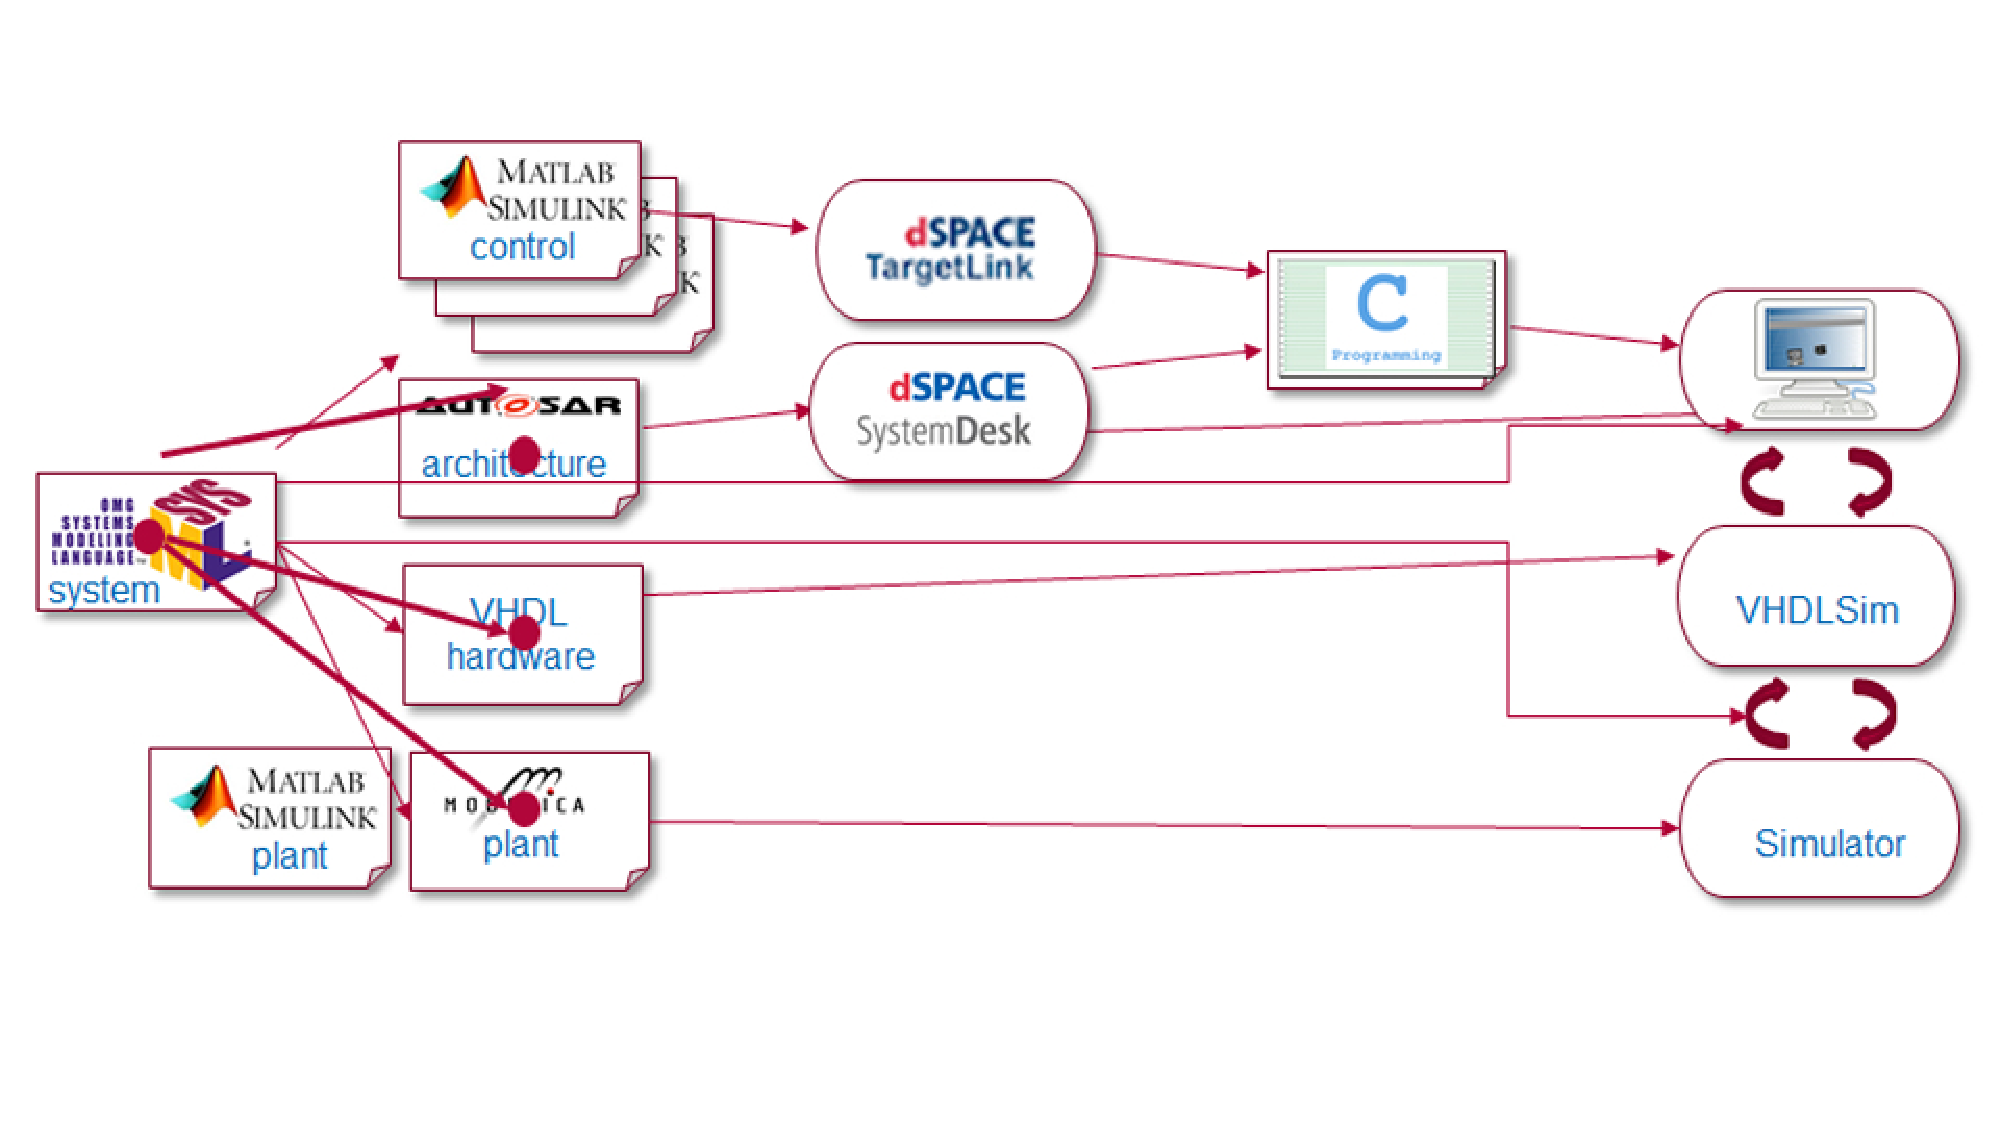
\includegraphics[scale=0.33]{figures/mm-hpi16.pdf}
\caption{Scenario: More Complex Horizontal Integration}
\label{fig:MMFig14}
\end{figure}

{\bf Scenario: More Complex Horizontal Integration } Figure~\ref{fig:MMFig14}

\begin{enumerate}
    \item Horizontal combination of multiple specific structures (Autosar: software; VHDL: hardware, Matlab/Modelica: plant) via a generic structure (SysML) 
\item Downwards propagation can be expected, but must be managed
\item Upwards propagation is usually forbidden (suppressed)
\item Horizontal propagation is therefore also forbidden (suppressed)
\item Vertical decomposition via a generic system structure (SysML) containing multiple specific structures (Matlab: control; Autosar: software; VHDL: hardware, Matlab/Modelica: plant; ...)
\item Consistency between models and in the models interact, which may lead to transitive propagation/conflicts
    
\end{enumerate}

}

\LATER[need for integration]{

% =========================================
\subsection{OPTIONAL?}

KKKKKKK

In order to discuss the role of MPM for CPS as present in the case study, we at first review the inherent integration needs underlying the development of embedded real-time systems and cyber-physical systems in particular based on the finding of \cite{GieseNNS2011}.

% ============================================
\subsubsection{Need for Integration}
%
As outline in \cite{GieseNNS2011} in more detail, the integration of separate parts of a system under development is tackled by a combination of (a) composition, (b) abstraction, and (c) consistency. As depicted in Figure~\ref{fig:MMFig1}, 

.

\begin{figure}[!htb]
\centering
%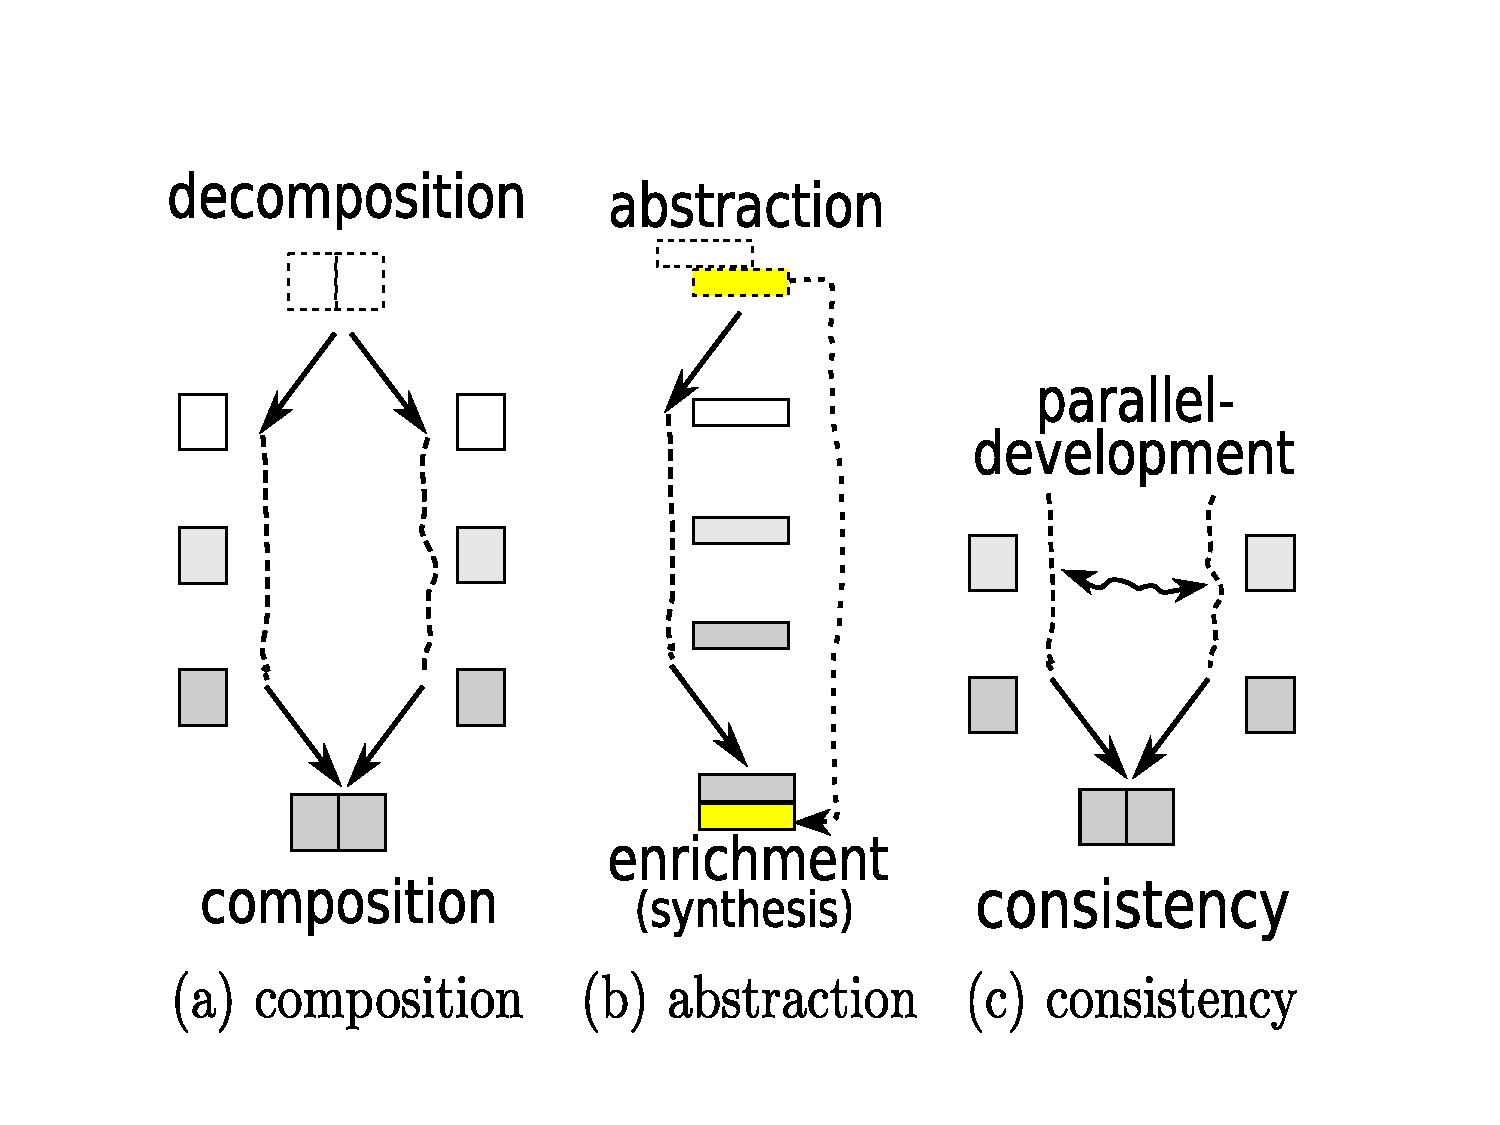
\includegraphics[scale=0.33]{figures/MM-Figure-1.pdf}
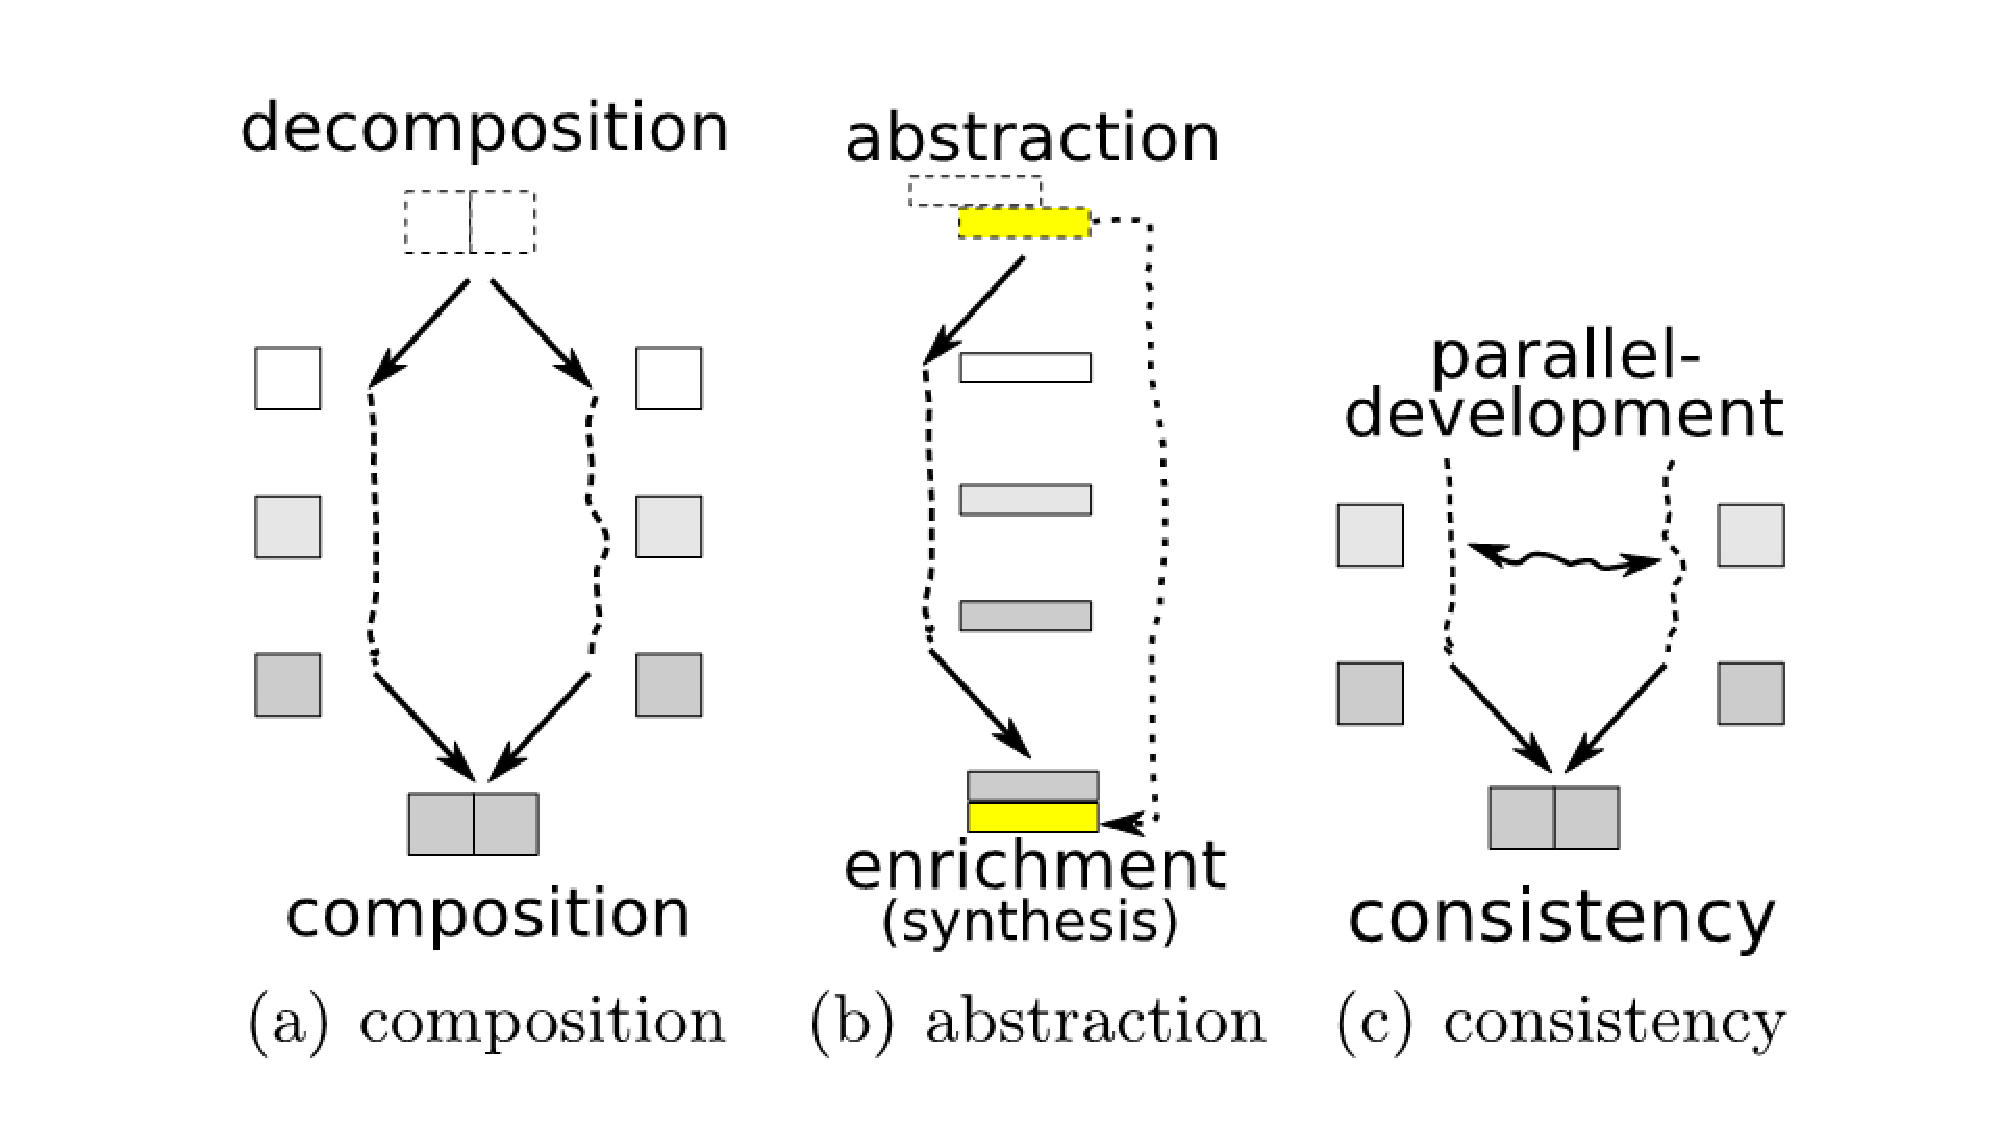
\includegraphics[scale=0.33]{figures/mm-hpi1.pdf}
\caption{Integration: 
When and  How (from~\cite{GieseNNS2011})}
\label{fig:MMFig1}
\end{figure}



% =========================================
\subsubsection{Enrichment}

KKKKKKKKK

\begin{figure}[!htb]
\centering
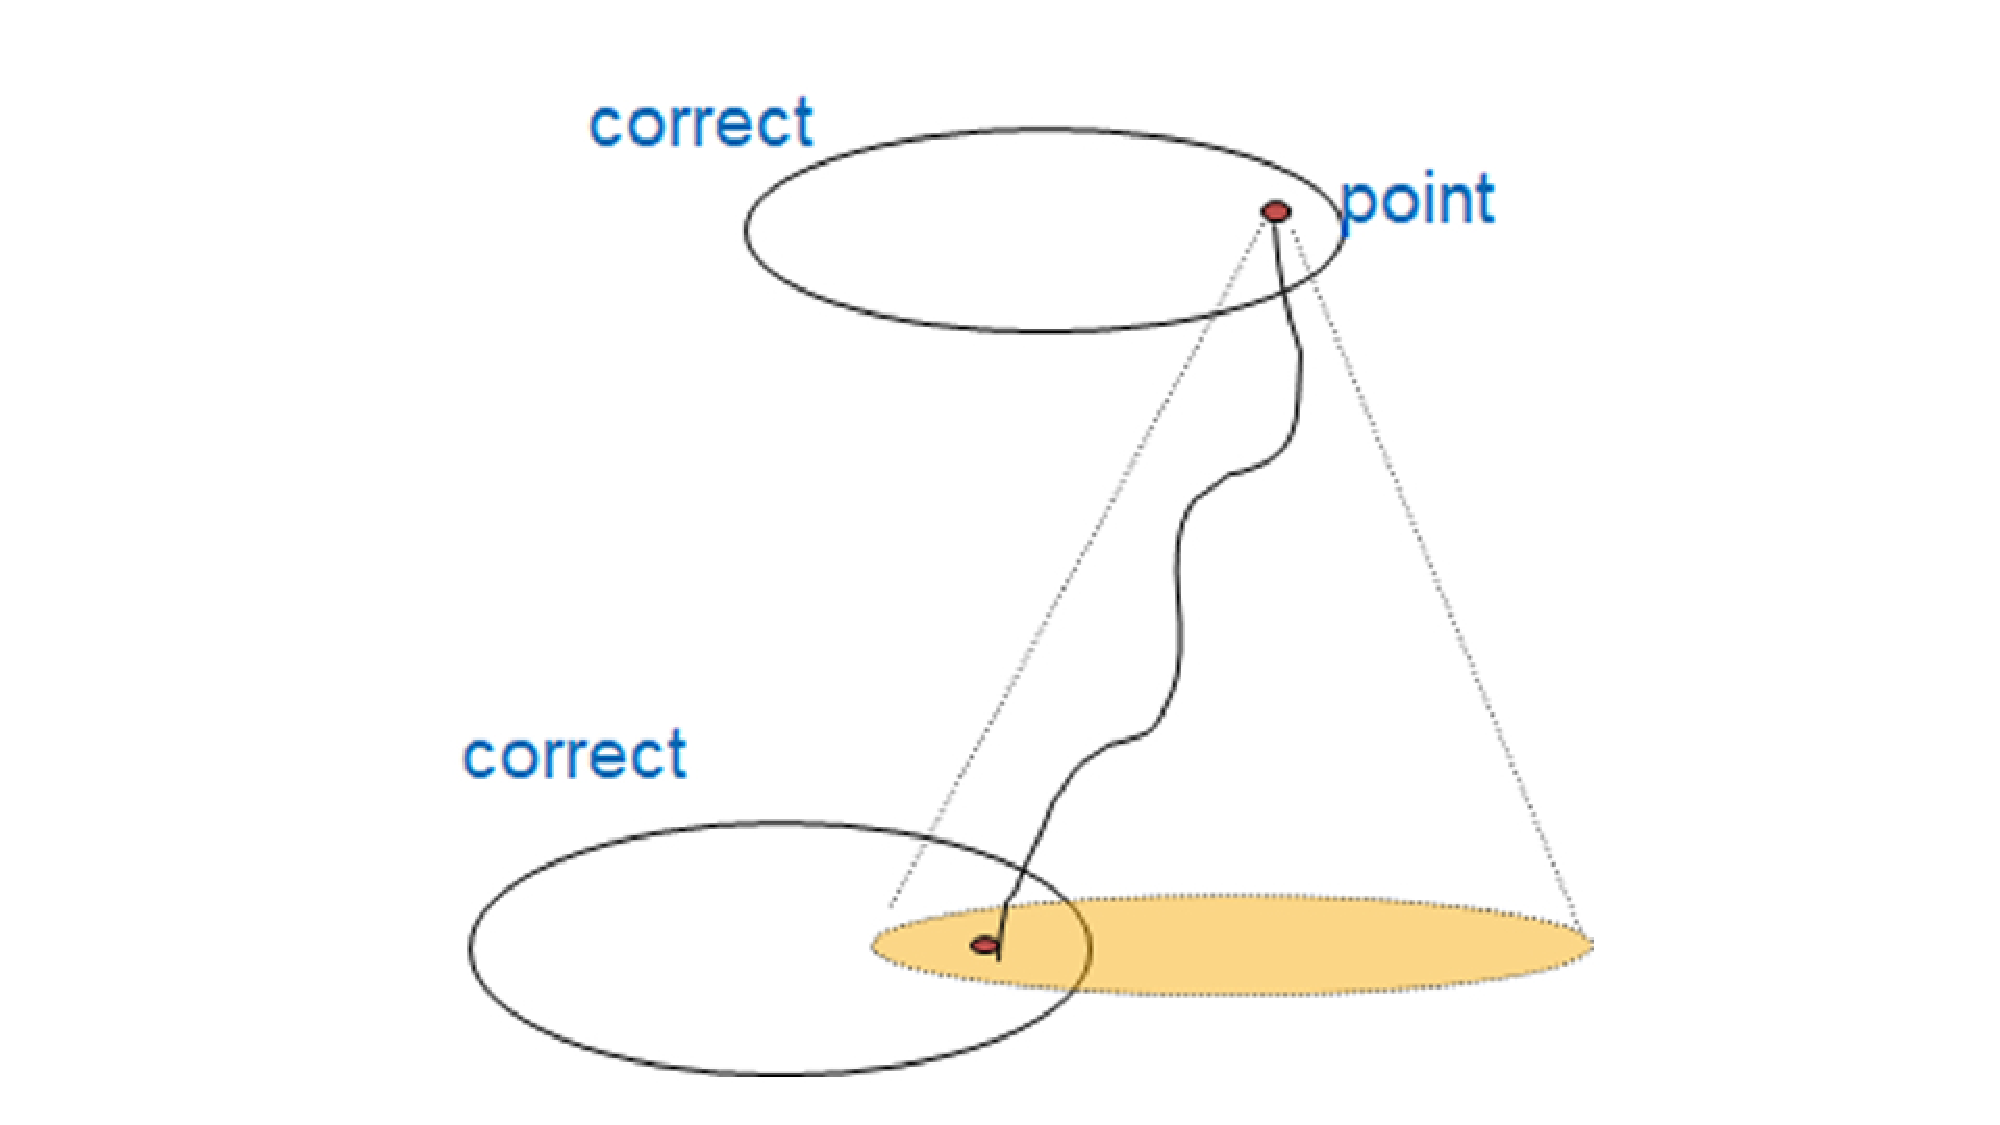
\includegraphics[scale=0.33]{figures/mm-hpi19.pdf}
\caption{Example for Approximation: Control}
\label{fig:MMFig15}
\end{figure}

{\bf Control:}

\begin{enumerate}
    \item Design an idealized control algorithm that assumes a continuous behavior in form of a differential equation (infinite fast; no discretization errors; $\ldots$)
\item Analyze that the idealized control algorithm provides the required guarantees (stability)
\item The later implemented control software and its timing is then tuned until it behaves as required (which is usually possible!)
\end{enumerate}


{\bf Approximation:}

\begin{enumerate}
    \item Ignore later details via idealization
\item Do not preserve relevant properties, but assumes that later considered details can be somehow handled
\item Optimistic approach: a solution for the problems raised by the later considered details will likely be found

\end{enumerate}



\begin{figure}[!htb]
\centering
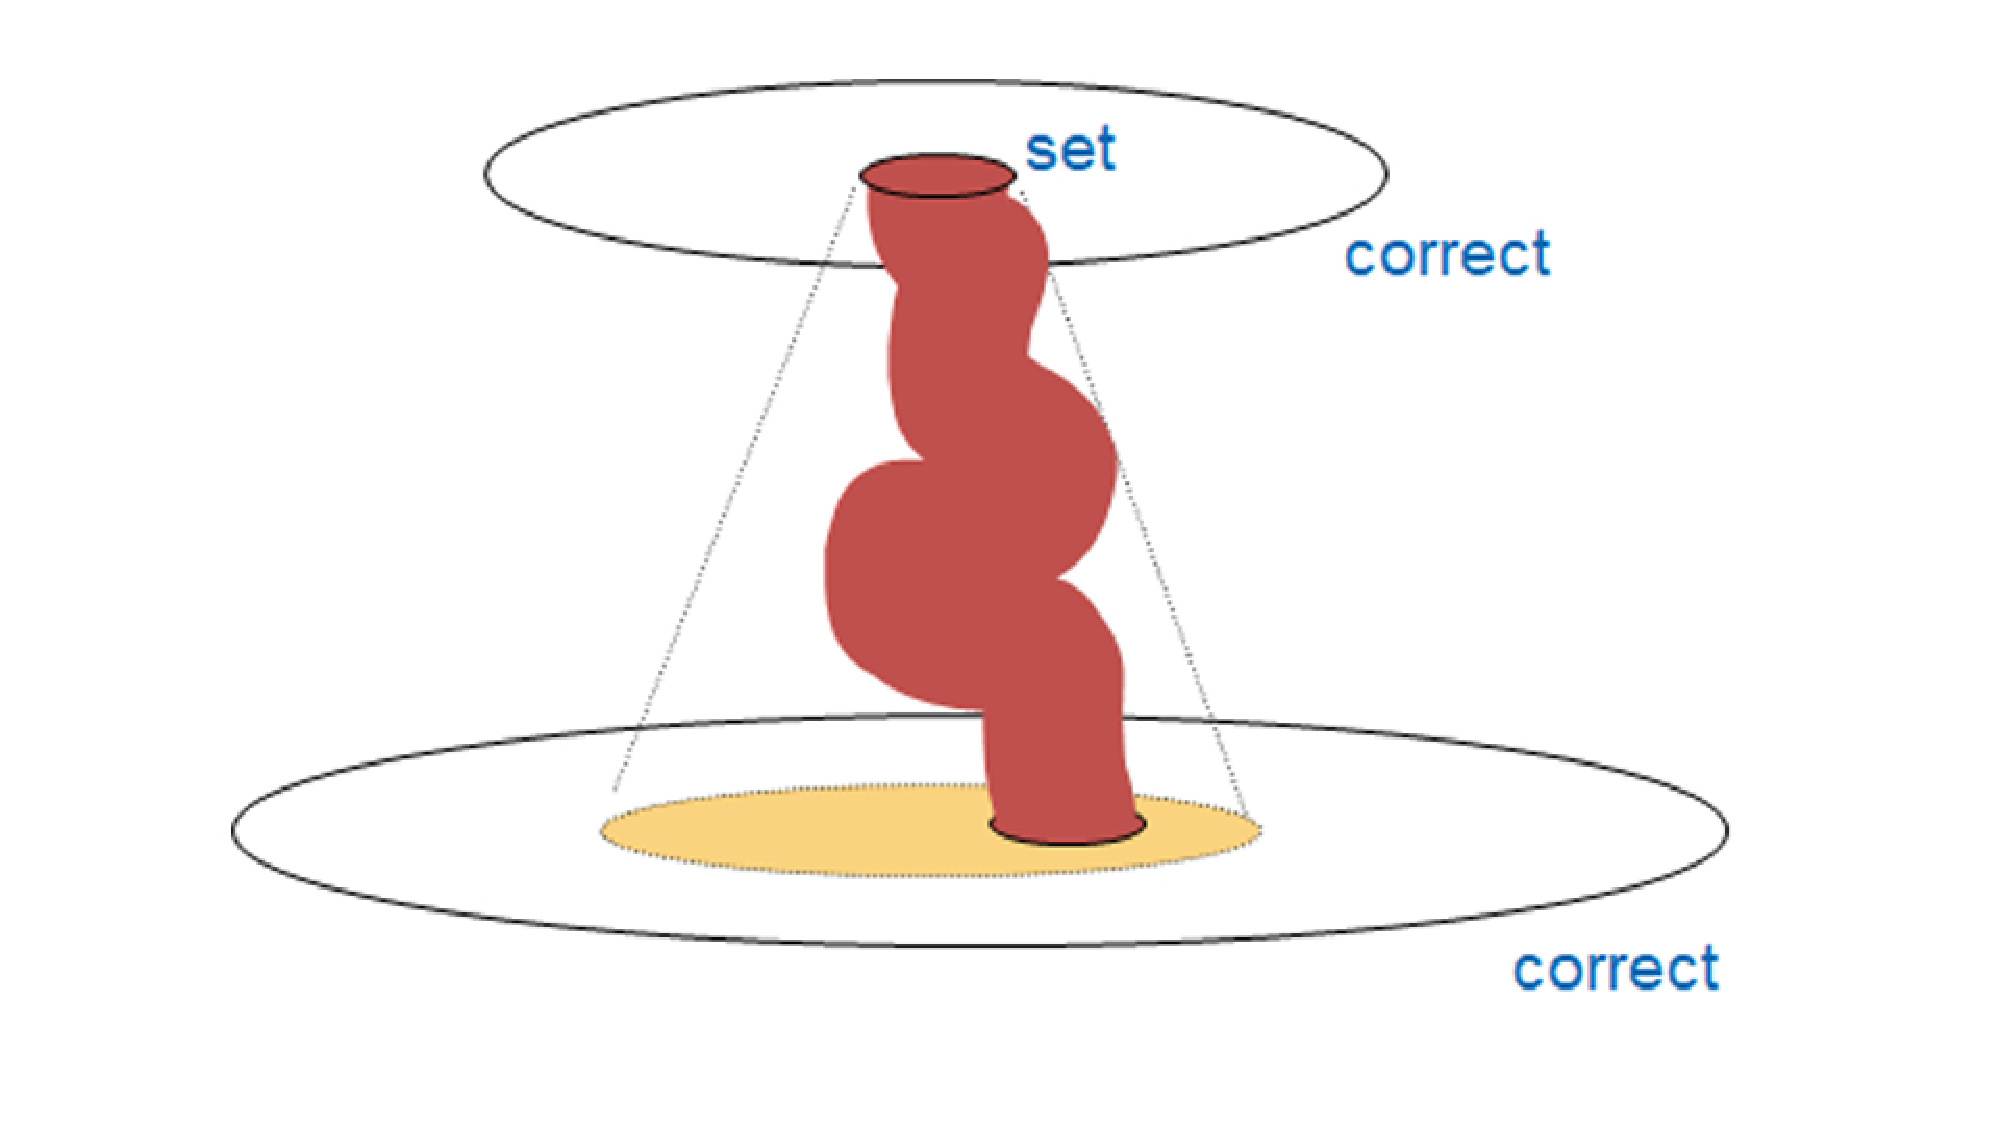
\includegraphics[scale=0.33]{figures/mm-hpi20.pdf}
\caption{Example for Refinement: Protocols}
\label{fig:MMFig16}
\end{figure}

{\bf Protocol:}

\begin{enumerate}
    \item Design an abstract model of a protocol that captures all possible message delays 
\item Verify that the abstract model guarantees the properties required for the protocol
\item The concrete protocol with specific time delays for messages will then be a refinement and thus also guarantees the required properties.
\end{enumerate}

{\bf Refinement:}

\begin{enumerate}
    \item Abstract from later details in a pessimistic manner
\item Preserve relevant properties
\item Pessimistic approach: 
exclude errors in later stages to be on the safe side
    
\end{enumerate}




\begin{figure}[!htb]
\centering
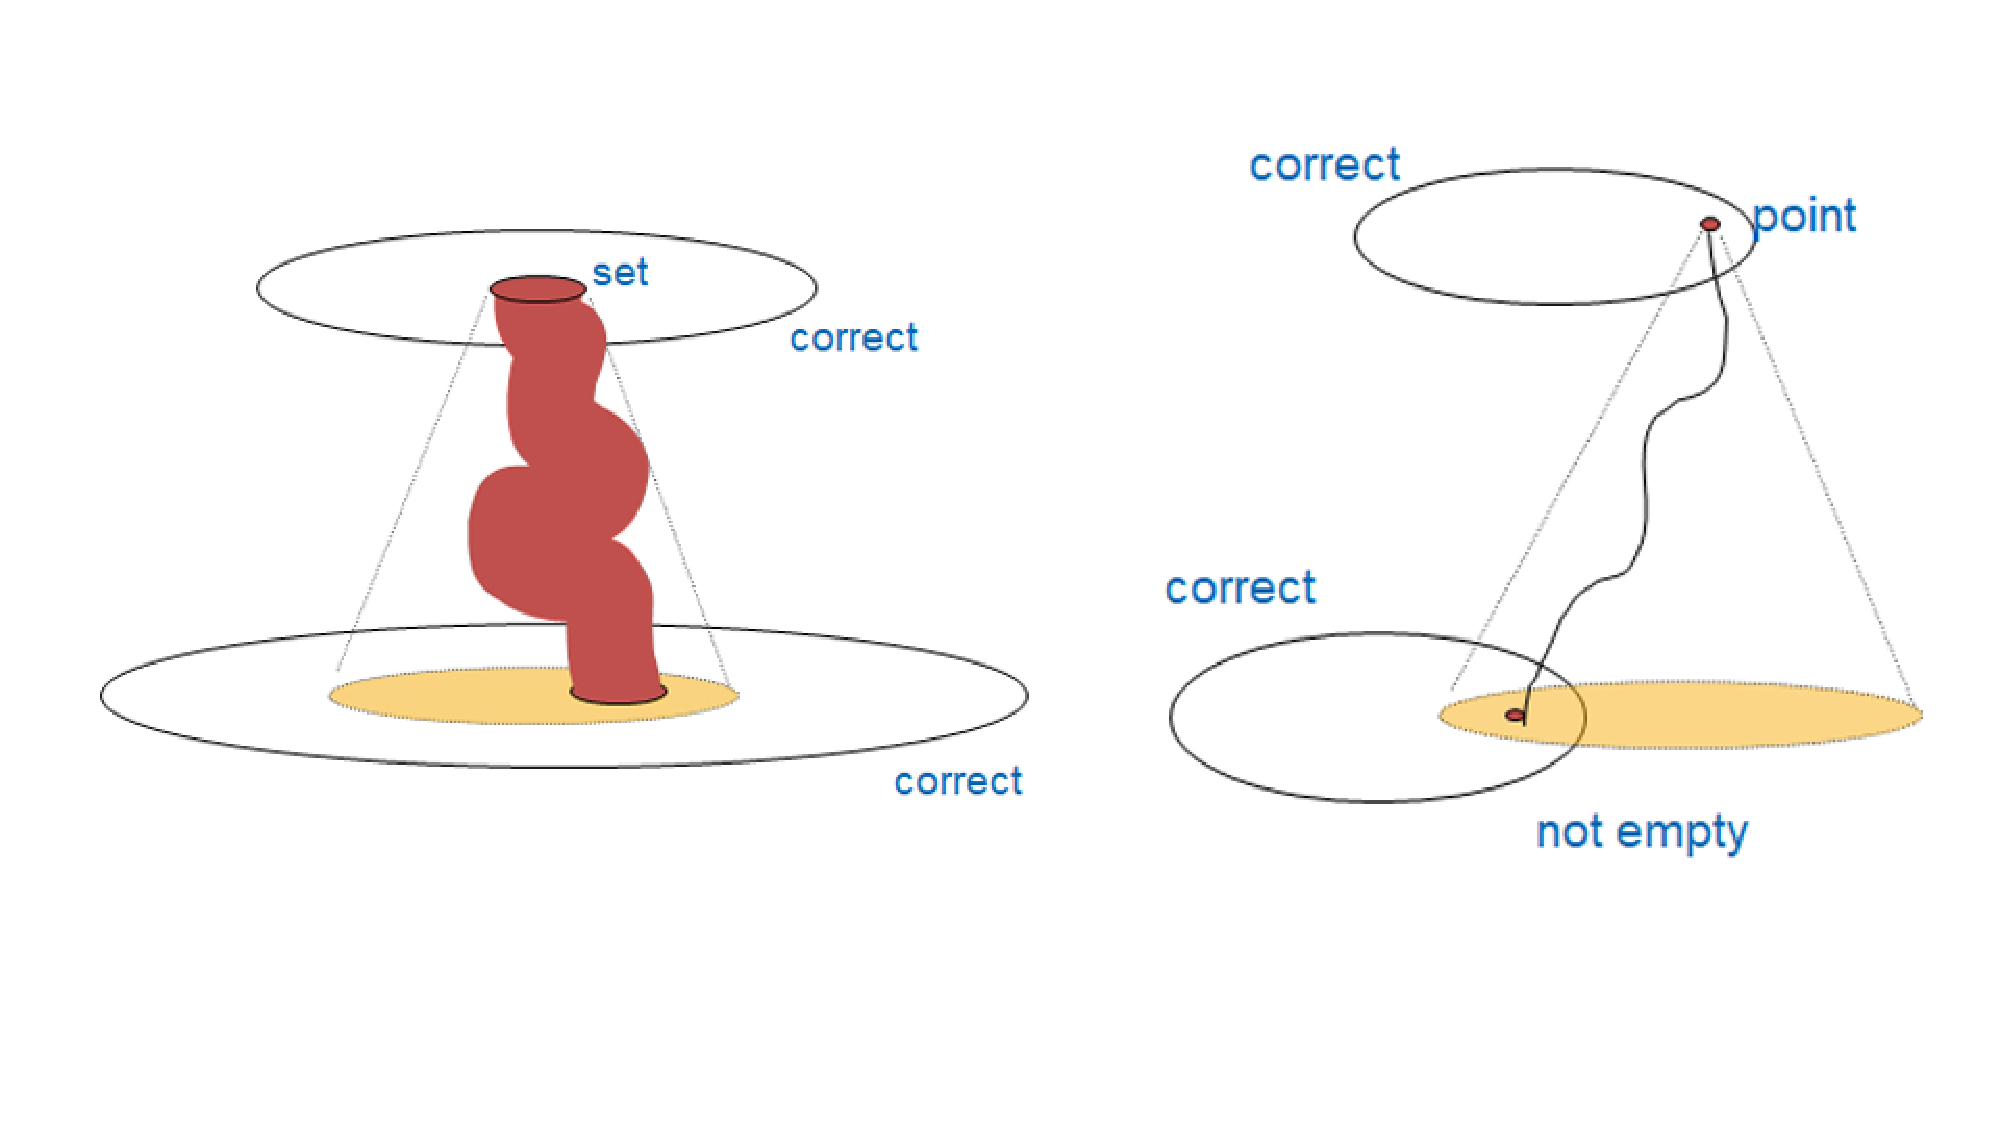
\includegraphics[scale=0.33]{figures/mm-hpi21.pdf}
\caption{Refinement vs. Approximation}
\label{fig:MMFig17}
\end{figure}

{\bf Approximation:}

\begin{enumerate}
    \item Ignore later details via idealization
\item Do not preserve relevant properties, but assumes that later considered details can be somehow handled
\item Optimistic approach: a solution for the problems raised by the later considered details will likely be found
    
\end{enumerate}

{\bf Refinement:}

\begin{enumerate}
    \item Abstract from later details in a pessimistic manner
\item Preserve relevant properties
\item Pessimistic approach: 
exclude errors in later stages to be on the safe side
\end{enumerate}


}

% ============================================
%\subsubsection{Use of MPM4CPS Ontology}\label{subsubsec:cpslab-mpm4cps-use}
%
\TODONOTE{ HG: Which MPM4CPS concept are required to describe the linkage between the MegaModelFragments with its models  from the MPM ontology and the CPS concepts from the CPS ontology?}

% ===============================================
\subsection{Summary}
%
We have demonstrated that the framework introduced in this report is 
%
suitable to capture the needs concerning this case study for CPS in form of the extensions of the CPS ontology discussed in  Section~\ref{subsec:cpslab-cps},
%
covering the needs concerning this case study for MPM in form of the extensions of the MPM ontology and the catalog discussed in  Section~\ref{subsec:cpslab-mpm}, and
%
captures the cyber-physical aspects of the development quite well as outlined in  Section~\ref{subsec:cpslab-mpm4cps}.

